%%%% utfpr-thesis.tex, 2024/02/10
%%%% Copyright (C) 2021-2024 Luiz E. M. Lima (luizeduardomlima@gmail.com)
%%
%% This work may be distributed and/or modified under the conditions of the
%% LaTeX Project Public License, either version 1.3 of this license or (at your
%% option) any later version.
%% The latest version of this license is in
%%   http://www.latex-project.org/lppl.txt
%% and version 1.3 or later is part of all distributions of LaTeX version
%% 2005/12/01 or later.
%%
%% This work has the LPPL maintenance status `maintained'.
%%
%% The Current Maintainer of this work is Luiz E. M. Lima.
%%
%% This work consists of all files listed in readme.html.
%%
%% A brief description of this work is in readme.txt.

%% Detecção e aviso sobre comandos obsoletos
% \RequirePackage[l2tabu, orthodox]{nag}

%% Classe de documento
\documentclass[%% Opções (^ = padrão; > = para pacotes; ¹ = somente twoside):
  a4paper,%% Tamanho de papel: a4paper, letterpaper (^), etc.
  12pt,%% Tamanho de fonte: 10pt (^), 11pt, 12pt, etc.
  oneside,%% Impressão de folhas: oneside ou twoside (^)
%   openany,%% Impressão de capítulos (¹): openany ou openright (^)
%   fleqn,%% Alinhamento de equações à esquerda (centralizado por padrão)
%   draft,%% Aparência de documento (>): draft ou final (^)
  brazilian,%% Idioma secundário (penúltimo) (>)
  english,%% Idioma primário (último) (>)
]{memoir}

%% Pacotes utilizados
\usepackage[%% Opções (^ = padrão; ¹ = somente twoside; ² = somente openany):
%   Font    = Times,%% Fonte principal: Arial (^), CM (padrão TeX) ou Times
%   Link    = TextColor,%% Cor de hyperlinks: DarkBlue (^) ou TextColor
%   Caption = Left,%% Alinhamento de legendas: Center (^) ou Left
%   Source  = Left,%% Alinhamento de fonte (referência): Center (^) ou Left
%   ABNTCit = NSB,%% Citação ABNT: AAY (Nome, Ano) (^), NRB (1) ou NSB [1]
%   BibDOI  = Icon,%% Ícone de DOI em referências: Icon ou Name (^)
%   BibURL  = Icon,%% Ícone de URL em referências: Icon ou URL (^)
%   CoverBG = On,%% Plano de fundo (capa e contracapa): On ou Off (^)
%   CoverId = All,%% Dados de identificação (capa): All ou Main (^)
%   PageNum = All,%% Numeração de páginas (partes): All, Main (^) ou None
%   TwoSide = All,%% Frente e verso (partes) (¹): All, Main (^) ou None
%   OpenPg  = Odd,%% Paginação de elementos (²): Odd ou Any (^)
%   Version = Defense,%% Versão de documento: Final (^) ou Defense
]{utfpr-thesis}
\usepackage[section]{placeins}

%% Informações do documento: descomentar para alterar
%%%% Título: {Em Português}; {In English}
\Title{%
    RMT 2.0: Uma ferramenta para aplicar e identificar padrões de projetos fundamentada em microsserviços
}{%
   RMT 2.0: A Tool for the Application and Identification of Design Patterns Based in Microservices%
}
%%%% Subtítulo (opcional): {Em Português}; {In English}
% \SubTitle{%
%   subtítulo de trabalho acadêmico%
% }{%
%   subtitle of academic work%
% }
%%%% Aluno(s) (de 1 a 5): {Número}; {Dados}
\Student{1}{%
   Gender   = {Male},%% Ou {Female}
   Forename = {Pedro Magnus Pedroso},%% Exceto último e sufixo (e.g., {José Santos da})
   Surname  = {Nogueira},%% Último e sufixo (e.g., {Silva Júnior})
%   Email    = {student1@domain},%% Opcional
%   Lattes   = {0000000000010001},%% Opcional
%   ORCID    = {0000-0000-0001-0001},%% Opcional (CHKTEX 8)
}
%%%% Grau acadêmico (opção): [Número] (Obs.: (¹) automático para cada opção)
% \AcademicDegreeOption[1]%% Doutorado
 \AcademicDegreeOption[2]%% Mestrado
% \AcademicDegreeOption[3]%% Especialização
% \AcademicDegreeOption[4]%% Bacharelado
% \AcademicDegreeOption[5]%% Licenciatura
% \AcademicDegreeOption[6]%% Tecnologia
%%%%%% Grau acadêmico (¹): {Em Português}; {In English}
% \AcademicDegree{Doutorado}{Doctorate}
%%%%%% Título acadêmico (¹): {Em Português}; {In English}
% \AcademicTitle{Doutor\Gen{a}}{Doctor}
%%%%%% Tipo de documento (¹): {Em Português}; {In English}
\DocumentType{Tese}{Thesis}
%%%% Área de concentração (Doutorado e Mestrado): {Em Português}; {In English}
\ConcentrationArea{Sistemas de informação e computação}{Information and Computer Systems}
%%%% Curso(s): {Em Português}; {In English}
\Course{Ciência da Computação}{Computer Science}
%%%% Departamento(s), coordenação(ões) ou programa: {Em Português}; {In English}
\Department{%
   Programa de Pós-Graduação em Ciência da Computação%
}{%
   Computer Science Graduate Program%
}
%%%% Campus: {Cidade}
\Campus{Ponta Grossa}
%%%% Ano(s) (atual por padrão): [De Depósito] (opcional); {De Defesa}
\Year[2024]{2024}

%% Processamento de entradas (itens) de listas, glossários e índices (makeindex)
%% Comandos \MakeAcronyms* e \MakeSymbols*: inserem as subdivisões da lista.
%%%% Lista de abreviaturas e siglas: [Arquivo de Entradas] (opcional)
% \MakeAcronyms[./Pre-Textual/Optionals/acronyms-entries]
%%%% Lista de símbolos: [Arquivo de Entradas] (opcional)
% \MakeSymbols[./Pre-Textual/Optionals/symbols-entries]
%%%% Glossário: [Arquivo de Entradas] (opcional)
% \MakeGlossary[./Post-Textual/Optionals/glossary-entries]
%%%% Índice remissivo
\MakeIndex%

%% Permissão de inclusão de arquivos: descomentar aqueles em edição
\includeonly{%
  ./Chapter-1/chapter-1,%% Capítulo 1 (CHKTEX 26)
  ./Chapter-2/chapter-2,%% Capítulo 2 (CHKTEX 26)
  ./Chapter-3/chapter-3,%% Capítulo 3 (CHKTEX 26)
  ./Chapter-4/chapter-4,%% Capítulo 4 (CHKTEX 26)
  ./Chapter-5/chapter-5,%% Capítulo 5 (CHKTEX 26)
  ./Post-Textual/appendix-a,%% Apêndice A (CHKTEX 26)
  ./Post-Textual/appendix-b,%% Apêndice B (CHKTEX 26)
  ./Post-Textual/annex-a,%% Anexo A (CHKTEX 26)
  ./Post-Textual/annex-b,%% Anexo B (CHKTEX 26)
}

%% Arquivo(s) de referências
\addbibresource{./Post-Textual/references.bib}

%% Início do documento
\begin{document}%% Não comentar ou remover

%% Capa (automática)
%% Para inserir planos de fundo na capa e em uma contracapa:
%% a) selecionar a opção do pacote utfpr-thesis: CoverBG = On;
%% b) atribuir nas informações do documento argumentos válidos para:
%%    - grau acadêmico (\AcademicDegreeOption[Número]);
%%    - campus (\Campus{Cidade}).

%% Elementos pré-textuais (frontmatter)
%% Editar o {Arquivo} para alterar: folha de rosto, errata, folha de aprovação,
%% dedicatória, agradecimentos, epígrafe, resumo e abstract.
%%%% ELEMENTOS PRÉ-TEXTUAIS
%%
%% Parte que antecede o texto com informações que ajudam na identificação e na
%% utilização do trabalho.
%%
%% Observações:
%% 1. {Arg} argumento obrigatório de ambiente ou comando.
%% 2. [Arg] argumento opcional de ambiente ou comando.

%% Folha de rosto
%% Contém os elementos essenciais à identificação do trabalho, além de uma
%% licença Creative Commons (https://creativecommons.org/choose/).
%% Ambiente {TitlePage*}: aplica caixa alta no título em idioma secundário.
\begin{TitlePage}%% Argumentos (2):
[BY]%% Tipo de licença (BY, BY-SA, BY-ND, BY-NC, BY-NC-SA ou BY-NC-ND)
% [Texto da licença]%% Substitui o texto padrão para cada tipo de licença
%%%% Descrição do trabalho (padrão; alterar se necessário)
\DocumentTypeName\ presented as requirement to obtain the title of \StudentsTitlesList\ in \CourseName\ from \ifbool{MakeAcr}{\intldescr{UTFPR} (\intl{UTFPR})}{\UTFPRName\ (UTFPR)}.
%%%% Orientador(es) (de 1 a 3): {Número}; {Dados}
\Advisor{1}{%
   Gender   = {Female},%% Ou {Female}
   Title    = {\ProfCall\ \PhDCall},%% {\<T>Call}; <T>: Prof/PhD/DSc/MSc/Eng
   Fullname = {Simone Nasser Matos},%% Conforme o Currículo Lattes
%   Email    = {advisor1@domain},%% Opcional
%   Lattes   = {0000000000020001},%% Opcional
%   ORCID    = {0000-0000-0002-0001},%% Opcional (CHKTEX 8)
}
\Advisor{2}{
   Gender   = {Female},%% Ou {Female}
   Title    = {\ProfCall\ \PhDCall},%% {\<T>Call}; <T>: Prof/PhD/DSc/MSc/Eng
   Fullname = {Helyane Bronoski Borges},%% Conforme o Currículo Lattes
%   Email    = {advisor1@domain},%% Opcional
%   Lattes   = {0000000000020001},%% Opcional
%   ORCID    = {0000-0000-0002-0001},%% Opcional (CHKTEX 8)
}
%%%% Ficha catalográfica (somente para Teses e Dissertações em catálogo físico)
%%%% [Arg-1]: local (pasta) do PDF (./Pre-Textual/Extras/ por padrão).
%%%% {Arg-2}: nome do PDF (modelo em ./Pre-Textual/Extras/).
% \IndexCardPDF{doc-index-card.pdf}
\end{TitlePage}

%% Errata (elemento opcional; editar o {Arquivo} para alterar)
% %%%% ERRATA (ELEMENTO OPCIONAL)
%%
%% Lista dos erros ocorridos no texto, seguidos das devidas correções.

%% Errata
%% Ambiente {Errata*}: insere a autorreferência do documento.
\begin{Errata}%[Título Alternativo]%% Substitui o título padrão
%%%% Formato (com \midrule entre linhas): Página(s) & Onde se lê & Leia-se \\
\labelcpageref{err:chpt-1,err:chpt-2,err:chpt-3,err:chpt-4,err:chpt-5,err:chpt-6} &
capítulo{(s)}                                                                     &
seção{(ões)} primária{(s)}                                                        \\
\midrule%
\pageref{err:ssect}         &
subseção{(ões)}             &
seção{(ões)} terciária{(s)} \\
\end{Errata}


%% Folha de aprovação
%% Contém os elementos essenciais à aprovação do trabalho (sem as assinaturas).
%%%% Opção 1: gerada por meio do pacote utfpr-thesis.
%%%% Ambiente {ApprovalPage*}: insere a titulação após o nome do membro.
%\begin{ApprovalPage}%% Argumentos (4):
% [brazilian]%% Idioma original ou primário (brazilian ou english)
%{Month Day, Year}%{August 14, \YearNum}%% Data de aprovação (dia, mês por extenso e ano)
%{14/08/\YearNum}%% Data de aprovação (forma abreviada; mestrado e doutorado)
%{\linewidth}%% Largura de linha de assinatura (graduação e especialização)
%%%%%% Descrição do trabalho (padrão; alterar se necessário)
%\DocumentTypeName\ presented as requirement to obtain the title of \StudentsTitlesList\ em \CourseName\ da \ifbool{MakeAcr}{\intldescr{UTFPR} (\intl{UTFPR})}{\UTFPRName\ (UTFPR)}.
%%%%%% Membro(s) da banca (de 3 a 6): {Número}; {Dados}
% \Member{1}{%
%   Gender      = {Female},%% Ou {Female}
%   Title       = {\ProfCall\ \PhDCall},%% {\<T>Call}; <T>: Prof/PhD/DSc/MSc/Eng
%   Fullname    = {Simone Nasser Matos (Advisor)},%% Conforme o Currículo Lattes
%   Institution = {\UTFPRName},%% Nome completo e por extenso
% }
% \Member{2}{%
%   Gender      = {Female},%% Ou {Male}
%   Title       = {\ProfCall\ \PhDCall},%% {\<T>Call}; <T>: Prof/PhD/DSc/MSc/Eng
%   Fullname    = {Leticia Mara Peres},%% Conforme o Currículo Lattes
%   Institution = {Federal University of Paraná},%% Nome completo e por extenso
% }
% \Member{3}{%
%   Gender      = {Female},%% Ou {Male}
%   Title       = {\ProfCall\ \PhDCall},%% {\<T>Call}; <T>: Prof/PhD/DSc/MSc/Eng
%   Fullname    = {Simone do Rocio Senger de Souza},%% Conforme o Currículo Lattes
%   Institution = {University of São Paulo},%% Nome completo e por extenso
% }
% \end{ApprovalPage}
%%%% Opção 2: gerada a partir do Sistema Acadêmico ou da secretaria.
%%%% [Arg-1]: local (pasta) do PDF (./Pre-Textual/Extras/ por padrão).
%%%% {Arg-2}: nome do PDF (modelos em ./Pre-Textual/Extras/).
\ApprovalPagePDF{doc-approval-page.pdf}

%% Dedicatória (elemento opcional; editar o {Arquivo} para alterar)
% %%%% DEDICATÓRIA (ELEMENTO OPCIONAL)
%%
%% Texto (pessoal) em que se presta homenagem ou se dedica o trabalho.

%% Dedicatória
\begin{Dedication}%% Argumentos (2):
% [0.5\textheight]%% Deslocamento vertical a partir da margem superior
% [Título]%% Não se aplica
%%%% Texto
Dedico este trabalho a minha família e aos meus amigos, pelos momentos de ausência.
\end{Dedication}


%% Agradecimentos (elemento opcional; editar o {Arquivo} para alterar)
%%%% AGRADECIMENTOS (ELEMENTO OPCIONAL)
%%
%% Texto (pessoal) em que se fazem agradecimentos dirigidos àqueles que
%% contribuíram de maneira relevante à elaboração do trabalho.

%% Agradecimentos
\begin{Acknowledgments}%[Título Alternativo]%% Substitui o título padrão
O presente trabalho não poderia ser finalizado sem a ajuda de diversas pessoas e/ou instituições às quais presto meus agradecimentos.
Certamente, esses parágrafos não abrangem todas as pessoas que fizeram parte dessa importante fase de minha vida.
Portanto, desde já peço desculpas àquelas que não estão presentes entre estas palavras, mas elas podem estar certas que fazem parte do meu pensamento com minha gratidão.\par%
A minha família, pelo carinho, incentivo e total apoio em todos os momentos da minha vida.\par%
Ao meu orientador, que me mostrou os caminhos a serem seguidos e pela confiança depositada.\par%
A todos os professores e colegas do curso, que ajudaram direta e indiretamente na realização e/ou conclusão deste trabalho.\par%
Aos demais que de alguma forma contribuíram para meu crescimento pessoal e profissional.\par%
%%%% À agência de fomento (último): {Nome}; {Número/Código do Fomento}
\FundingAgency{%
  da \ifbool{MakeAcr}{\intldescr{CAPES}}{Coordenação de Aperfeiçoamento de Pessoal de Nível Superior} \textemdash\ Brasil (\ifbool{MakeAcr}{\intl{CAPES}}{CAPES})%% CAPES
%   do \ifbool{MakeAcr}{\intl{CNPq}, \intldescr{CNPq}}{CNPq, Conselho Nacional de Desenvolvimento Científico e Tecnológico} \textemdash\ Brasil%% CNPq
%   da Fundação Araucária \textemdash\ Brasil%% FA
%   da \ifbool{MakeAcr}{\intl{UTFPR}, \intldescr{UTFPR}}{UTFPR, \UTFPRName} \textemdash\ Brasil%% UTFPR
}{%
  \textemdash\ Código de Financiamento 001%% CAPES
%   (\No\ de processo)%% CNPq
%   (\No\ de edital, financiamento, processo ou projeto)%% FA
%   (\No\ de edital, financiamento, processo ou projeto)%% UTFPR
}
\end{Acknowledgments}


%% Epígrafe (elemento opcional; editar o {Arquivo} para alterar)
% %%%% EPÍGRAFE (ELEMENTO OPCIONAL)
%%
%% Texto em que se apresenta uma citação, seguida de indicação de autoria,
%% relacionada com a matéria tratada no corpo do trabalho.

%% Opção 1: baseada na ABNT NBR 10520 (citações diretas curtas e longas).
%% Ambiente {Epigraph*}: remove o formato de citação direta longa.
\begin{Epigraph}%% Argumentos (2):
% [0.5\textheight]%% Deslocamento vertical a partir da margem superior
% [Título]%% Não se aplica
%%%% Epígrafes nos idiomas primário (texto) e original (nota de rodapé)
%%%% [Arg-1]: idioma (brazilian ou english).
%%%% {Arg-2}: autoria.
%%%% {Arg-3}: texto.
%%%% [Arg-4]: nota de rodapé.
\Citation[brazilian]{\cite[tradução própria]{Einstein1921}}{%
  Até onde as leis da matemática se referem à realidade, não são certas; e até onde são certas, não se referem à realidade
}[%
  \Citation[english]{\cite{Einstein1921}}{%
    As far as the laws of mathematics refer to reality, they are not certain; and as far as they are certain, they do not refer to reality
  }.
].
\par%
\Citation[brazilian]{\cite[\ppno~37, tradução própria]{Asimov1950}}{%
  Primeira Lei: um robô não pode ferir um ser humano ou, por omissão, permitir que um ser humano sofra algum mal.
  Segunda Lei: um robô deve obedecer às ordens que lhe sejam dadas por seres humanos, exceto nos casos em que tais ordens contrariem a Primeira Lei.
  Terceira Lei: um robô deve proteger sua própria existência desde que tal proteção não entre em conflito com a Primeira ou Segunda Leis
}[%
  \Citation[english]{\cite[37]{Asimov1950}}{%
    First Law: a robot may not injure a human being or, through inaction, allow a human being to come to harm.
    Second Law: a robot must obey the orders given it by human beings except where such orders would conflict with the First Law.
    Third Law: a robot must protect its own existence as long as such protection does not conflict with the First or Second Laws
  }.
].
\end{Epigraph}

%% Opção 2: baseada na classe de documento memoir.
% \begin{Epigraphs}%% Argumentos (2):
% [0.5\textheight]%% Deslocamento vertical a partir da margem superior
% [Título]%% Não se aplica
%%%% Epígrafes nos idiomas primário (texto) e original (nota de rodapé)
%%%% [Arg-1]: idioma (brazilian ou english).
%%%% {Arg-2}: autoria.
%%%% {Arg-3}: texto.
%%%% [Arg-4]: nota de rodapé.
% \EpiItem[brazilian]{\cite[tradução própria]{Einstein1921}}{%
%   Até onde as leis da matemática se referem à realidade, não são certas; e até onde são certas, não se referem à realidade.
% }[%
%   \Citation[english]{\cite{Einstein1921}}{%
%     As far as the laws of mathematics refer to reality, they are not certain; and as far as they are certain, they do not refer to reality
%   }.
% ]
% \end{Epigraphs}


%% Resumo
%% Apresentação concisa dos pontos relevantes de um texto, fornecendo uma visão
%% rápida e clara do conteúdo e das conclusões do trabalho.
%% Ambiente {Abstract*}: insere a autorreferência do documento.
%%%% Estilo de fonte da chamada das palavras-chave (opcional)
% \KeywordsCallFormat{\bfseries}%% Texto normal por padrão
%%%% Palavras-chave (de 3 a 6): {Número}; {Em Português}; {In English}
\Keyword{1}{refatoração de software}{software refactoring}
\Keyword{2}{padrões de projetos}{design patterns}
\Keyword{3}{microserviços}{microservices}
\Keyword{4}{processo semiautomatizado}{semi-automated process}
%%%% Em língua vernácula (idioma primário)
\begin{Abstract}[brazilian]%% Idioma (brazilian ou english)
Refatoração é um meio de melhorar o código-fonte sem alterar a sua funcionalidade, removendo code smells e tornando-o mais flexível e legível. Dentre as técnicas de refatoração, existe a refatoração por padrões de projetos que permite criar um código com maior qualidade em relação a atributos como reusabilidade, flexibilidade, entre outros. A ferramenta Refactoring and Measurement Tool (RMT) foi criada em sua primeira versão pelo Laboratório de Engenharia de Software e Inteligência Computacional (LESIC) e é capaz de ler um projeto escrito em linguagem java e detectar e aplicar padrões de projeto em linguagem Java. Para isso, ela contém a implementação de três métodos da literatura capazes de detectar e aplicar padrões de projeto. A dificuldade da primeira versão da RMT está relacionada em se incorporar em sua arquitetura uma quantidade maior de métodos. Este trabalho realizou a refatoração de código e de sua arquitetura. O processo de melhoramento da primeira versão da RMT abrangeu as fases de: análise, restruturação, testes, refatoração e avaliação. A arquitetura da RMT foi modificada usando microserviços assíncronos e nativos na nuvem para melhorar a performance, disponibilidade e escalabilidade, desacoplando as responsabilidades. Como resultado criou-se a versão da RMT 2.0 que contém um escalonamento horizontal para melhorar a performance sobre demanda, combinando com aplicações em nuvem. Os testes criados facilitam aos desenvolvedores realizarem modificações para estender a ferramenta. O código-fonte foi simplificado para trazer melhor performance a ferramenta e melhorar a experiência do desenvolvedor que deseja contribuir com a ferramenta. O processo de execução local da ferramenta foi alterado, trazendo melhora na facilidade do mecanismo de execução, podendo ser executada com containers. A análise dos resultados evidencia uma redução de 63.64\% de tempo de execução na refatoração dos projetos testados em relação a ferramenta original.

\end{Abstract}
%%%% Em língua estrangeira (idioma secundário; para divulgação internacional)
\begin{Abstract}[english]%% Idioma (brazilian ou english)
Refactoring enhances the integrity of the source code without altering its functionality, eliminating code smells while improving its flexibility and readability. Among the various refactoring techniques, using design patterns facilitates the development of higher-quality code with enhanced attributes such as reusability and flexibility. The Refactoring and Measurement Tool (RMT) was initially developed by the Software Engineering and Computational Intelligence Laboratory (LESIC) and is capable of parsing Java projects to detect and implement design patterns. This functionality is achieved by integrating three established methodologies from the literature. The primary challenge of the first version of RMT is its limited capacity to incorporate additional methodologies into its architectural framework. This work has done a comprehensive refactoring of both the codebase and the architecture. The enhancements to the initial version of RMT were executed in phases that included analysis, restructuring, testing, refactoring, and evaluation. The RMT architecture was reengineered using asynchronous, cloud-native microservices to boost performance, availability, and scalability while segregating responsibilities. Consequently, RMT 2.0 was developed, featuring horizontal scaling to meet the performance demands associated with cloud integration. The developed testing facilitates developer modifications to extend the tool's feature set.  The source code has been optimized to enhance the tool's performance, thereby improving the development experience for contributors. The tool's local execution process has been modified to streamline the execution mechanism by allowing container-based deployment. Empirical analysis of the results indicates a 63.64\% reduction in execution time during project refactoring compared to the original tool.
\end{Abstract}


%% Lista de algoritmos (elemento opcional)
% \PrintFloatsList{algorithm}

%% Lista de ilustrações (elemento opcional; lista geral)
% \PrintIllustrationsList{figure, flowchart, photograph, graph, tabframed}
%%%% Lista de figuras (usar a partir de 3 itens e remover da lista geral)
\PrintFloatsList{figure}
%%%% Lista de fluxogramas (usar a partir de 3 itens e remover da lista geral)
% \PrintFloatsList{flowchart}
%%%% Lista de fotografias (usar a partir de 3 itens e remover da lista geral)
% \PrintFloatsList{photograph}
%%%% Lista de gráficos (usar a partir de 3 itens e remover da lista geral)
% \PrintFloatsList{graph}
%%%% Lista de quadros (usar a partir de 3 itens e remover da lista geral)
% \PrintFloatsList{tabframed}

%% Lista de tabelas (elemento opcional)
\PrintFloatsList{table}

%% Lista de abreviaturas e siglas (elemento opcional)
%%%% Opção 1: makeindex; conforme o [Arquivo de Entradas] em \MakeAcronyms.
% \PrintAcronymsList%
%%%% Opção 2: manual; editar o {Arquivo} para alterar.
% %%%% LISTA DE ABREVIATURAS E SIGLAS (ELEMENTO OPCIONAL)
%%
%% Consiste na relação alfabética das abreviaturas e siglas utilizadas no texto,
%% seguidas das palavras ou expressões correspondentes grafadas por extenso.
%% Recomenda-se a elaboração de lista própria para cada tipo.

%% Lista de abreviaturas e siglas (inserir itens em ordem alfabética)
\begin{AcronymsList}%[Título Alternativo]%% Substitui o título padrão
\item[1D] Unidimensional
\item[ABNT] Associação Brasileira de Normas Técnicas
\item[Art.] Artigo
\item[BMP] Mapa de Bits (\ENLang*{Bitmap})
\item[Cap.] Capítulo
\item[CAPES] Coordenação de Aperfeiçoamento de Pessoal de Nível Superior
\item[CNPq] Conselho Nacional de Desenvolvimento Científico e Tecnológico
\item[CTAN] \ENLang{Comprehensive \TeX\ Archive Network}
\item[EPS] \ENLang{Encapsulated PostScript}
\item[GIF] Formato de Intercâmbio de Gráficos (\ENLang*{Graphics Interchange Format})
\item[GIMP] Programa de Manipulação de Imagem GNU (\ENLang*{GNU Image Manipulation Program})
\item[GNU] GNU Não é Unix (\ENLang*{GNU is Not Unix})
\item[JPEG] \ENLang{Joint Photographic Experts Group}
\item[NBR] Norma Brasileira
\item[PDF] Formato de Documento Portátil (\ENLang*{Portable Document Format})
\item[PNG] Gráficos Portáteis de Rede (\ENLang*{Portable Network Graphics})
\item[PS] \ENLang{PostScript}
\item[QR] Resposta Rápida (\ENLang*{Quick Response})
\item[Seç.] Seção
\item[TCC] Trabalho de Conclusão de Curso
\item[TUG] \ENLang{\TeX\ Users Group}
\item[UML] Linguagem de Modelagem Unificada (\ENLang*{Unified Modeling Language})
\item[URL] Localizador Uniforme de Recursos (\ENLang*{Uniform Resource Locator})
\item[UTF-8] Formato de Transformação Unicode de 8-bit (\ENLang*{8-bit Unicode Transformation Format})
\item[UTFPR] Universidade Tecnológica Federal do Paraná
\end{AcronymsList}


%% Lista de símbolos (elemento opcional)
%%%% Opção 1: makeindex; conforme o [Arquivo de Entradas] em \MakeSymbols.
%%%% Comando \PrintSymbolsList*: insere a unidade (entre []) na margem direira.
% \PrintSymbolsList%
%%%% Opção 2: manual; editar o {Arquivo} para alterar.
% %%%% LISTA DE SÍMBOLOS (ELEMENTO OPCIONAL)
%%
%% Conjunto de sinais que substituem o nome de uma coisa ou de uma ação.
%% Elaborada conforme a ordem apresentada no texto, com o devido significado.

%% Lista de símbolos (inserir itens em ordem de ocorrência)
\begin{SymbolsList}%[Título Alternativo]%% Substitui o título padrão
\item[\nu] Viscosidade cinemática, \Unit{m^2/s}
\item[\mu] Viscosidade dinâmica, \Unit{kg/{(m{}\cdot{}s)}}
\item[\rho] Massa específica, \Unit{kg/m^3}
\item[A] Área, \Unit{m^2}
\item[\pi] Constante circular (Pi), \Unit{rad}
\item[D] Diâmetro, \Unit{m}
\item[R] Raio, \Unit{m}
\item[\overline{\MrkSym}] Média temporal
\item[\langle\MrkSym\rangle] Média na seção transversal
\item[\vec{\nabla}] Operador gradiente
\item[\MrkSym^-] Passo de tempo anterior
\item[\MrkSym^+] Passo de tempo posterior
\item[\MrkSym^0] Valor inicial
\item[\MrkSym_\mathrm{G}] Fase gasosa
\item[\MrkSym_\mathrm{L}] Fase líquida
\item[\MrkSym_\mathrm{S}] Fase sólida
\item[\theta] Inclinação, \Unit{\Degree}
\item[L] Comprimento, \Unit{m}
\item[\mathrm{Re}] Número de Reynolds
\item[V] Velocidade, \Unit{m/s}
\end{SymbolsList}


%% Sumário
%% Comando \PrintSummary*: remove o espaçamento entre partes e entre capítulos.
\PrintSummary%

%% Formatação de elementos textuais (mainmatter)
\Textual%% Não comentar ou remover

%% Parte 1 (elemento opcional; grupo de capítulos)
% \part{Introdução}%
% \label{part:intro}

%% Capítulo 1
\chapter{Introduction}%
\label{chpt-intro}

The definition of refactoring is to modify a software code without changing its external behavior to improve its internal structure. It is applied carefully to minimize the possibility of introducing bugs into the already-written code. Refactoring does not depend on whether the code had a good design or if the software had no plan because, with refactoring, we can transform it into an excellent structure code \cite{fowler2018refactoring}.

Different types of refactoring exist, such as refactoring by techniques \cite{fowler2018refactoring} and refactoring with design patterns \cite{kerievsky2005refactoring}. Refactoring-based methods change the code structure to make it easier to understand and improve maintenance by removing code smells. Refactoring based on design patterns improves the code structure by inserting patterns.

The RMT is developed to integrate the existing literature concerning methodologies for code refactoring to implement design patterns. Several approaches conceived by the authors, such as strategy \cite{CHRISTOPOULOU20121201}, factory method and strategy \cite{liu2014automated}, NULL object \cite{GAITANI201533}, and template method \cite{zafeiris2017automated}. The articles provide methodologies and tools for identifying and incorporating specific design patterns as defined by \textcite{Gamma2009}.

\textcolor{red}{<<deve falar que para aplicar padrões de projetos existem métodos na litetura como os de X, Y e que cada um implementa o seu método. Porém, uma forma e integrar esses métodos foi a criação da RMT. Comentar sobre a RMT e citar comentar o problema que ela tem>>}

Multiple architecture options are available when designing systems, such as queues, REST (Representational State Transfer), RPC (Remote Procedure Call), etc. Microservices can combine those technologies to create large and complex architectures, as they have advantages over monolithic architecture, such as fault tolerance, organization, and development velocity \cite{microservices-comuni}. To implement such architecture, a cloud is an excellent option for its native tools, such as serverless computing, container managers, databases, and many other tools \cite{balalaie2016}.

\textcolor{red}{<<esta ligação dos dois parágrafos ficou confuso. Talvez falar que a RMT implements REST e depois comentar o problema que essa solucção tem>>}

\textcite{beluzzo2018abordagem} chose some technologies to create the RMT, such as REST communication and services, to divide the business logic. The tool is divided into three services, those been: detection service, metrics service, and intermediary service; its architecture communicates with REST requests over the intermediary service responsible for knowing all the services and making the load balance; that architecture can fit as microservices.

This work refactored the RMT architecture, bringing its design to a cloud-native approach with AWS (Amazon Web Services) working with offered services such as Elasticache for caching and storage, Fargate for container management, SQS (Simple Queue Service) as queue broker, and S3 for file storage. The refactor also includes a change from the synchronous approach to asynchronous by making the services communicate by queues and removing the responsibility of managing requests from the client to the service itself. In addition to architecture, the limitations detected in the tool will be fixed.

By transitioning to a cloud-based architecture, RMT 2.0 markedly enhances performance, scalability, and reliability. The improvements encompass asynchronous communication via queues, storage migration to Amazon S3 and Redis, and a streamlined package architecture using the Spring framework. The upgraded browser-based interface preserves the linear user interaction for project evaluation and refactoring. Empirical evaluations have substantiated the tool's efficacy in identifying refactoring candidates and enhancing metrics, with RMT 2.0 exhibiting superior performance and reduced execution times, notably in template method refactoring. Furthermore, the tool's deployment has had a 63.64\% improvement in time efficiency.


\textcolor{red}{<<colocar aqui de uma maneira geral os resultados>>}

\section{Justification}
Asynchronous microservices allow services to operate independently and scale horizontally without affecting other services. They can tolerate failures better than synchronous architectures, as they do not depend on each other's availability or response time. A failed microservice or request does not block the entire system; the different services can operate without interruption \cite{microservices-comuni}.

Asynchronous microservices can perform better than synchronous architectures by reducing latency and increasing throughput. Asynchronous processing allows the system to handle more requests concurrently and more efficiently. The microservice architecture enables greater flexibility in technology choices and enables services to be written in different programming languages, frameworks, and libraries. This architecture also allows for better integration with third-party services and APIs \cite{larrucea2018}.

Consequently, refactoring the RMT tool improves the end-user experience, rendering it faster and more reliable than its previous version. The developer's advantages post-refactoring are evident when the tool is executed within a modern framework and integrated with Docker, ensuring a seamless setup. Furthermore, restructuring the packages and classes results in a more concise codebase, thereby improving the developer's comprehension and maintainability of the tool. Given that the tool incorporates extensive unit testing, the developer can verify that modifications will not compromise the functionality of other methods since the test suite can be executed consistently to verify integrity.

\textcolor{red}{<<comentar o que o desenvolvedor vai ganhar>>. Como os microserviços ajudam na extensão da ferramenta para outros métodos e métricas}.

\section{Objective}
Refactor the RMT to an asynchronous and cloud-native architecture to make the tool scalable, resulting in a better experience for the end user.

The specific objectives are: i) build an async architecture and cloud-native; ii) refactor the code to work with threads; iii) refactor the java version and framework; iv) compare the refactored tool with the existing one; v) create unit and integration tests.

% Obejetivo geral e especifico
\section{Methodology}
As systematic reviews had already been conducted by \textcite{beluzzo2018abordagem} on detection and application design patterns, in this work, a forward snowball technique was used to search for new articles in the field of refactoring, not exclusively for application design patterns. Through this process, it was discovered that there were no new works on this topic, confirming the need to improve an RMT tool.

\textcolor{red}{contar o que fez depois do snowballing - sempre em algo nível: 1 - estudo da ferramenta RMT para entender seu funcionamento, 2 -..... Acho que o parágrafo seguinte deve ser revisto}

The methodology process is divided into five phases: analyzing, restructuring, testing, refactoring, and evaluating the tool. It is described into five sequentially interconnected phases; each phase systematically uses the insights and understanding obtained from the previous stage to optimize its efficacy.
 
The methodology includes various analyses and refactoring strategies for multiple services within the tool. These services include the Intermediary Service, the Detection Service, and the Metrics Service, each intensively analyzed and tested before being restructured and renamed for better clarity and functionality. Cloud technologies like S3, Redis, and AWS SQS were used to improve performance and scalability. Extensive unit tests were incorporated to ensure reliability during the refactoring process.

\section{Work Organization}

This work is divided into four chapters that present the refactoring of the RMT architecture into an async tool. The \cref{cap-background} talks about refactoring, the RMT tool, and microservices.

In \cref{chap-state} details the state of the art with a forward snowballing about refactoring, tools, and methods.

In \cref{methodology}, the methodology used to achieve the result of the refactoring is described in detail.

In \cref{results}, the findings are systematically explained and critically analyzed to fulfill the research objectives.

In \cref{conclusion}, the final synthesis of the research is presented.

%% Parte 2 (elemento opcional; grupo de capítulos)
% \part{Desenvolvimento}%
% \label{part:dev}

%% Capítulo 2
\chapter{Theoretical Background}
\label{cap-background}

As \textcite{fowler2018refactoring} described, refactoring is the design improvement after writing a code. Refactoring opportunities may arise throughout the project's development regardless of how the project was carried out, especially in systems developed by teams.

Refactoring seeks to remove code smells encountered in software development; when software becomes mature and evolves, two conflicts arise: i) The software needs to fulfill all requirements, and ii) The software's reusability. Implementing new functionality to the software without refactoring is possible, but eventually, it will take great effort \cite{Gamma2009}.

Refactoring can facilitate the implementation of new requirements, modularize overloaded classes, and find methods and unnecessary classes. Different types of refactoring exist, such as techniques or methods based on design patterns. \textcite{fowler2018refactoring} is one of the most known authors. He created a catalog separating refactorings into seven (7) groups and making it available for consulting. Fowler's online catalog encompasses the refactorings described in his two books: Refactoring: Improving the Design of Existing Code \cite{fowler2018refactoring} and Refactoring: Ruby Edition \cite{fields2009refactoring}. 

Refactoring by designing pattern-based methods examines the source code for insertion points to apply patterns. This refactoring aims mainly at maintainability, readability, and reusability. Several authors propose their pattern-based refactoring methods, such as \textcite{cinneide2000automated}, \textcite{Gamma2009}, and \textcite{ouni2017more}.

This chapter has information about the research background. \Cref{sec-importance} discuss the importance of refactoring. \Cref{sec-methods} describes the application of refactoring. \Cref{sec-tools} exemplifies the methods of refactoring and the explanations of its functionalities and tools. \Cref{sub-rmt} talks about RMT functionality. \Cref{sub-architecture} describes the tool architecture. \Cref{subsub-internal} talks about the internal functionality of RMT. \Cref{sub-usage} shows how to use the tool. \Cref{subsub-limitation} discusses the limitations encountered using the tool. \Cref{sec-microservices} explain about microservices. \Cref{sec2-remarks} includes the final considerations.

\section{Importance of Software Refactoring}
\label{sec-importance}
\textcite{fowler2018refactoring} describes that the first step in refactoring is to create automated tests such as unit tests. The tests help to avoid creating bugs by guaranteeing that the behavior does not change, as any code change could also change the code behavior; humans may make mistakes and cause severe problems in production. In system production, maintainability is a significant factor that influences costs, and one of the proposed solutions to reduce it is to increase software quality. 

Refactoring can be applied to the development process to increase software quality, forcing the programmer to find bad smells (a characteristic of the code that indicates an issue) \cite{Wilking2007}. 
In the study of \textcite{szHoke2017empirical}, six systems were analyzed to verify the effectiveness of software refactoring aimed at maintainability. To obtain the data before the refactorings, \textcite{szHoke2017empirical} analyzed all systems using a code analyzer called SourcerMeter tool based on the Columbus tool \cite{ferenc2002}. Refactorings were done manually, and the developers were informed about all the data and the list of problematic code fragments. 

In this study, the developers analyzed 2.5 million lines and performed 732 revisions to the code, of which 315 were refactorings and 1,273 refactorings operations. After finishing the analyses, \textcite{szHoke2017empirical} found that refactoring improved maintainability, and the tool improved 5 out of 6 tested systems. In conclusion, the study shows that refactoring improves maintainability, which helps in fulfilling future software requirements.

\subsection{Methods to Apply refactoring}
\label{sub-methods}
As mentioned, we can apply refactoring techniques and methods based on design patterns. Refactoring by techniques is common and can be found in the leading IDEs, such as Eclipse and IntelliJ, which provides automatic refactorings based on the model created by \textcite{fowler2018refactoring}. 

Several authors propose software refactoring methods applying patterns, each performed differently in refactorings using pattern-based design methods. Some of these authors are \textcite{liu2014automated}, \textcite{zafeiris2017automated}, \textcite{cinneide2000automated}, and \cite{ouni2017more}. 
These refactoring methods seek to find pattern insertion points in the source code. The technique searches source code to find where to implement design patterns to improve code maintainability, readability, and reusability. 

As distinct from technical refactoring, design pattern-based refactoring looks for parts of the code where a design pattern can be applied. Using a design pattern is very important because it makes the evolution of the software more natural and does not create problems when implementing new requirements. Several project patterns have different functionality, such as factory method, proxy, observer, adapter, visitor, builder, and others \cite{Gamma2009}). 

As described in the mapping performed by \textcite{beluzzo2018abordagem}, several authors propose methods for refactorings based on design patterns. For example, in the Moore method and Minipatterns and Minitransformations, there is a tool for each implementation process. If the developer wants to refactor his source code, he has to run n tools, where n is the total number of methods.

The focus of refactoring by design patterns is different from refactoring by techniques. Refactoring by design patterns tries to find a way to make a system easy to "update." Software with difficulties in being "updated" can cost a lot to the company, both in terms of value and needs for new clients and competitiveness with other companies \cite{cinneide2000automated}.

\subsection{Methods and Tools for Refactoring Based on Design Patterns}
\label{sec-tools}

As mentioned, \textcite{beluzzo2018abordagem} identified methods for detecting and involving design patterns as described in \Cref{tab-articles}.


\begin{tabframed}[!htbp]
\caption{Articles with design patterns methods}
\label{tab-articles}
\begin{tabularx}{\textwidth}{|e{}@{},{}@{}|p{3cm}|p{8cm}|c|c@{}|}
%% Cabeçalho da primeira página
\toprule%
\multicolumn{1}{|@{}c|}{\textbf{Key}}             &
\multicolumn{1}{c|}{\textbf{Author}}             &
\multicolumn{1}{c|}{\textbf{Title}}              &
\multicolumn{1}{c|}{\textbf{Year}}               &
\multicolumn{1}{c@{}|}{\textbf{Has Tool}}        \\
\midrule%
A1  & \citeauthor*{GAITANI201533}            & Automated refactoring to the Null Object design pattern                                                             & 2015 & Yes      \\
A2  & \citeauthor*{CHRISTOPOULOU20121201}    & Automated refactoring to the Strategy design pattern                                                                & 2012 & Yes      \\
A3  & \citeauthor*{zafeiris2017automated}           & Automated refactoring of super-class method invocations to the Template Method design pattern                       & 2017 & Yes      \\
A4  & \citeauthor*{CINNEIDE2015}             & A multi-objective refactoring approach to introduce design patterns and fix anti-patterns                           & 2015 & Yes      \\
A5  & \citeauthor*{cinneide2001automated}    & Automated application of design patterns: a refactoring approach                                                    & 2001 & Yes      \\
A6  & \citeauthor*{cinneide792644}           & A Methodology for the automated introduction of design patterns                                                     & 1999 & Yes      \\
A7  & \citeauthor*{mens972774}               & A declarative evolution framework for object-oriented design patterns                                               & 2001 & Yes      \\
A8  & \citeauthor*{sang1183003}              & An automated refactoring approach to design pattern-based program transformations in Java programs                  & 2002 & Yes      \\
A9  & \citeauthor*{Cinneide602499}           & Automated Software Evolution Towards Design Patterns                                                                & 2001 & Yes      \\
A10 & \citeauthor*{cinneide337612}           & Automated refactoring to introduce design patterns                                                                  & 2000 & Yes      \\
A11 & \citeauthor*{Liu2014}                  & Automated pattern-directed refactoring for complex conditional statements                                           & 2014 & No       \\
A12 & \citeauthor*{ram2004detecting}         & Detecting Intent Aspects from Code to Apply Design Patterns in Refactoring: An Approach Towards a Refactoring Tool  & 2004 & Yes      \\
A13 & \citeauthor*{hotta6178876}             & Identifying, tailoring and suggesting form template method refactoring Opportunities with program dependence graph. & 2012 & Yes      \\
A14 & \citeauthor*{rajesh1013988}            & JIAD: A tool to infer design patterns in refactoring                                                                & 2004 & Yes      \\
A15 & \citeauthor*{ouni2017more}             & MORE: A multi-objective refactoring recommendation approach to introducing design patterns and fixing code smells   & 2017 & Yes      \\
A16 & \citeauthor*{eden632834}               & Precise specification and automatic application of design patterns                                                  & 1997 & No       \\
A17 & \citeauthor*{kerievsky2005refactoring} & Refactoring to Patterns                                                                                             & 2008 & No       \\
A18 & \citeauthor*{kim7332467}               & Scripting parametric refactorings in java to retrofit design patterns                                               & 2015 & No       \\
A19 & \citeauthor*{kim2014scripting}         & Scripting Refactorings in Java to Introduce Design Patterns                                                         & 2014 & Yes      \\
A20 & \citeauthor*{juillerat4362900}         & Toward an implementation of the ”Form Template Method” Refactoring                                                  & 2007 & Yes      \\
A21 & \citeauthor*{ajouli6619484}            & Transformations between composite and visitor implementations in Java                                               & 2013 & Yes     \\
\bottomrule%
\end{tabularx}
\SourceOrNote{adapted from \textcite{beluzzo2018abordagem}}
\end{tabframed}
\FloatBarrier

For each of the papers, there are methods to recognize design pattern insertions, but not every article has a tool to apply it as described in \Cref{tab-articles}. \textcite{beluzzo2018abordagem} searched for the papers until 2018 when his work was published; a new search was made with the same search strings and libraries from 2019 to 2023, and no new work was found.

Some steps ought to be taken to refactor code and apply transformations, as refactoring is not a straightforward technique and may vary by who is using it. That is why the authors have taken different approaches to refactoring listed on \Cref{tab-refactoring}.

\begin{table}[!htbp]
\caption{Refactoring Types}%
\label{tab-refactoring}
\begin{tabularx}{\textwidth}{e{},{}@{}lX@{}}
\toprule%
\multicolumn{1}{@{}c}{\textbf{Keys}}  &
\multicolumn{1}{c@{}}{\textbf{Types}} \\
\midrule%
A15, A10, A9, A6, A5 & MiniTransformations                                        \\
A2, A11              & Conditional Expression Refactorings                        \\
A12, A14             & Intent Aspects Refactoring*                                \\
A18, A19             & Reflective Refactorings                                    \\
A4, A15, A21         & Composite to Visitor and Visitor to Composite Refactorings \\
A4, A7, A15          & Role based Refactorings                                    \\
\bottomrule%
\end{tabularx}
\SourceOrNote{adapted from \textcite{beluzzo2018abordagem}}
\end{table}
\FloatBarrier


A refactoring type will apply to the code for every work, as described in \Cref{tab-refactoring}.

I) Minitransformations are he minitransformation is simple modifications to the code; by grouping those transformations in the right way, a design pattern is created \cite{cinneide2001automated}. II) Reflective Refactoring is based on code reflections, a technique that allows the code to be changed on runtime. It's good to emphasize that there are no pre-refactoring implementations with reflections; they are a method to implement the refactorings \cite{beluzzo2018abordagem}. III) Role Role-based refactoring is defined by a group of roles corresponding to the pattern participants and applying those roles to refactor obtaining design pattern \cite{mens972774}. IV) Intent Aspects are aspects in the software susceptible to pattern refactoring, formed by a group of rules for each pattern\cite{ram2004detecting}. V) Composite to Visitor and Visitor to Composite: focus only on the transition between each pattern \cite{beluzzo2018abordagem}. VI) Conditional Expression Refactorings: focus on the code's conditional expressions and conditional branches to refactor. \cite{CHRISTOPOULOU20121201}

As shown on \Cref{tab-articles}, most of the articles have tools, and those were developed to apply the methods described above, working in an automatic or semi-automatic manner.

\begin{table}[!htbp]
\caption{Developed tools}%
\label{tab-tools}
\begin{tabularx}{\textwidth}{e{},{}@{}lX@{}}
\toprule%
\multicolumn{1}{@{}c}{\textbf{Keys}}  &
\multicolumn{1}{c@{}}{\textbf{Tools}} \\
\midrule%
A2, A3         & JDeodorant                   \\
A4             & MORE                         \\
A6, A7, A8, A9 & Prototype\textbf{*}          \\
A5, A10        & Design Pattern Tool          \\
A13            & Creios                       \\
A12, A15       & JIAD                         \\
A15            & MORE                         \\
A11, A19, A20  & Eclipse Plugin\textbf{*}     \\
A21            & JHotDraw                     \\
\bottomrule%
\end{tabularx}
\SourceOrNote{adapted from \textcite{beluzzo2018abordagem}}
\end{table}
\FloatBarrier

In \Cref{tab-tools}, the tools developed are listed by name; the row marked by an asterisk means that the tool is a prototype or an eclipse plugin; the other articles were created or updated of a specific tools\cite{beluzzo2018abordagem}.

The tool creation is necessary because manual refactoring, the process some developers use, can introduce errors to the code and even change the system's functionality. This problem happens because developers are not prepared to perform refactoring \cite{ge2012reconciling}.

Manual refactoring needs reviewing the entire code, and it can take time. For this reason, tools facilitate the application of refactorings, which can act in identifying bad smells or identifying and refactoring the source code, as created by \textcite{beluzzo2018abordagem}.

\textcite{beluzzo2018abordagem} performed a mapping to find refactoring techniques and several tools have already been developed to perform refactorings. Such as Elbereth \cite{korman1998elbereth}, which automates some code extraction refactorings, encompassing method extraction (Extract Method), abstract superclasses, replacement of an existing class, and addition of a new subclass.

Aiming at the interaction with the user for the application of refactoring, \cite{murphy2008breaking} created a tool that is fast, resistant to errors, and that is pleasant to use. To make the tool enjoyable, they implemented markings in the code produced by rectangles, arrows, and coloring parts of the code. These three markings show the user cleanly where and what the problem is so that refactorings can be applied.
There are also tools containing a graphical interface and iteration with the user, such as \textcite{rani2014detection}, where the intent is to detect bad smells. This tool was developed in C\# and finds bad smells like long method, large class, lazy class, and comment lines. Discovering smells in code written in JAVA and .net. 

Many code refactoring tools are based on the catalog of refactorings created by \cite{fowler2018refactoring}. However, other authors propose new refactorings. However, most authors agree that manually performed refactoring is time-consuming and challenging without creating new smells in the code. They were making tools for this reason.

\cite{murphy2008breaking}, together with eight software developers with different work experiences, used the GostFactor tool to assist in refactoring. They observed that this process decreased errors in the refactoring application by 23.3\%.

The RMT tool created by \textcite{beluzzo2018abordagem} allows for integrating design pattern insertion and detection methods in a single environment. The tool has an iteration with the user to let them know what will happen in the code after refactoring and, simultaneously, if the refactoring will improve the code. The work by \textcite{sangeetha2019empirical} does not describe how the implemented tool works but uses it to test and validate the techniques used. The RMT was created to implement the methods cited above. \textcite{beluzzo2018abordagem} implemented two methods, allowing the tool to extend to as many methods as possible.

\subsection{RMT}
\label{sub-rmt}

The RMT (Refactoring and Measurement Tool) tool was created to detect design pattern insertion points using the methods selected by the author \cite{beluzzo2018abordagem}. \textcite{zafeiris2017automated} and \textcite{liu2014automated} developed the already implemented refactoring methods. The method by \textcite{zafeiris2017automated} covers refactoring for the Template Method pattern, and the method by \textcite{liu2014automated} covers two patterns: Strategy and Factory Method.

\begin{figure}[ht!]
\SetCaptionWidth{\textwidth}
\caption{RMT use case}
\label{fig-usecase}
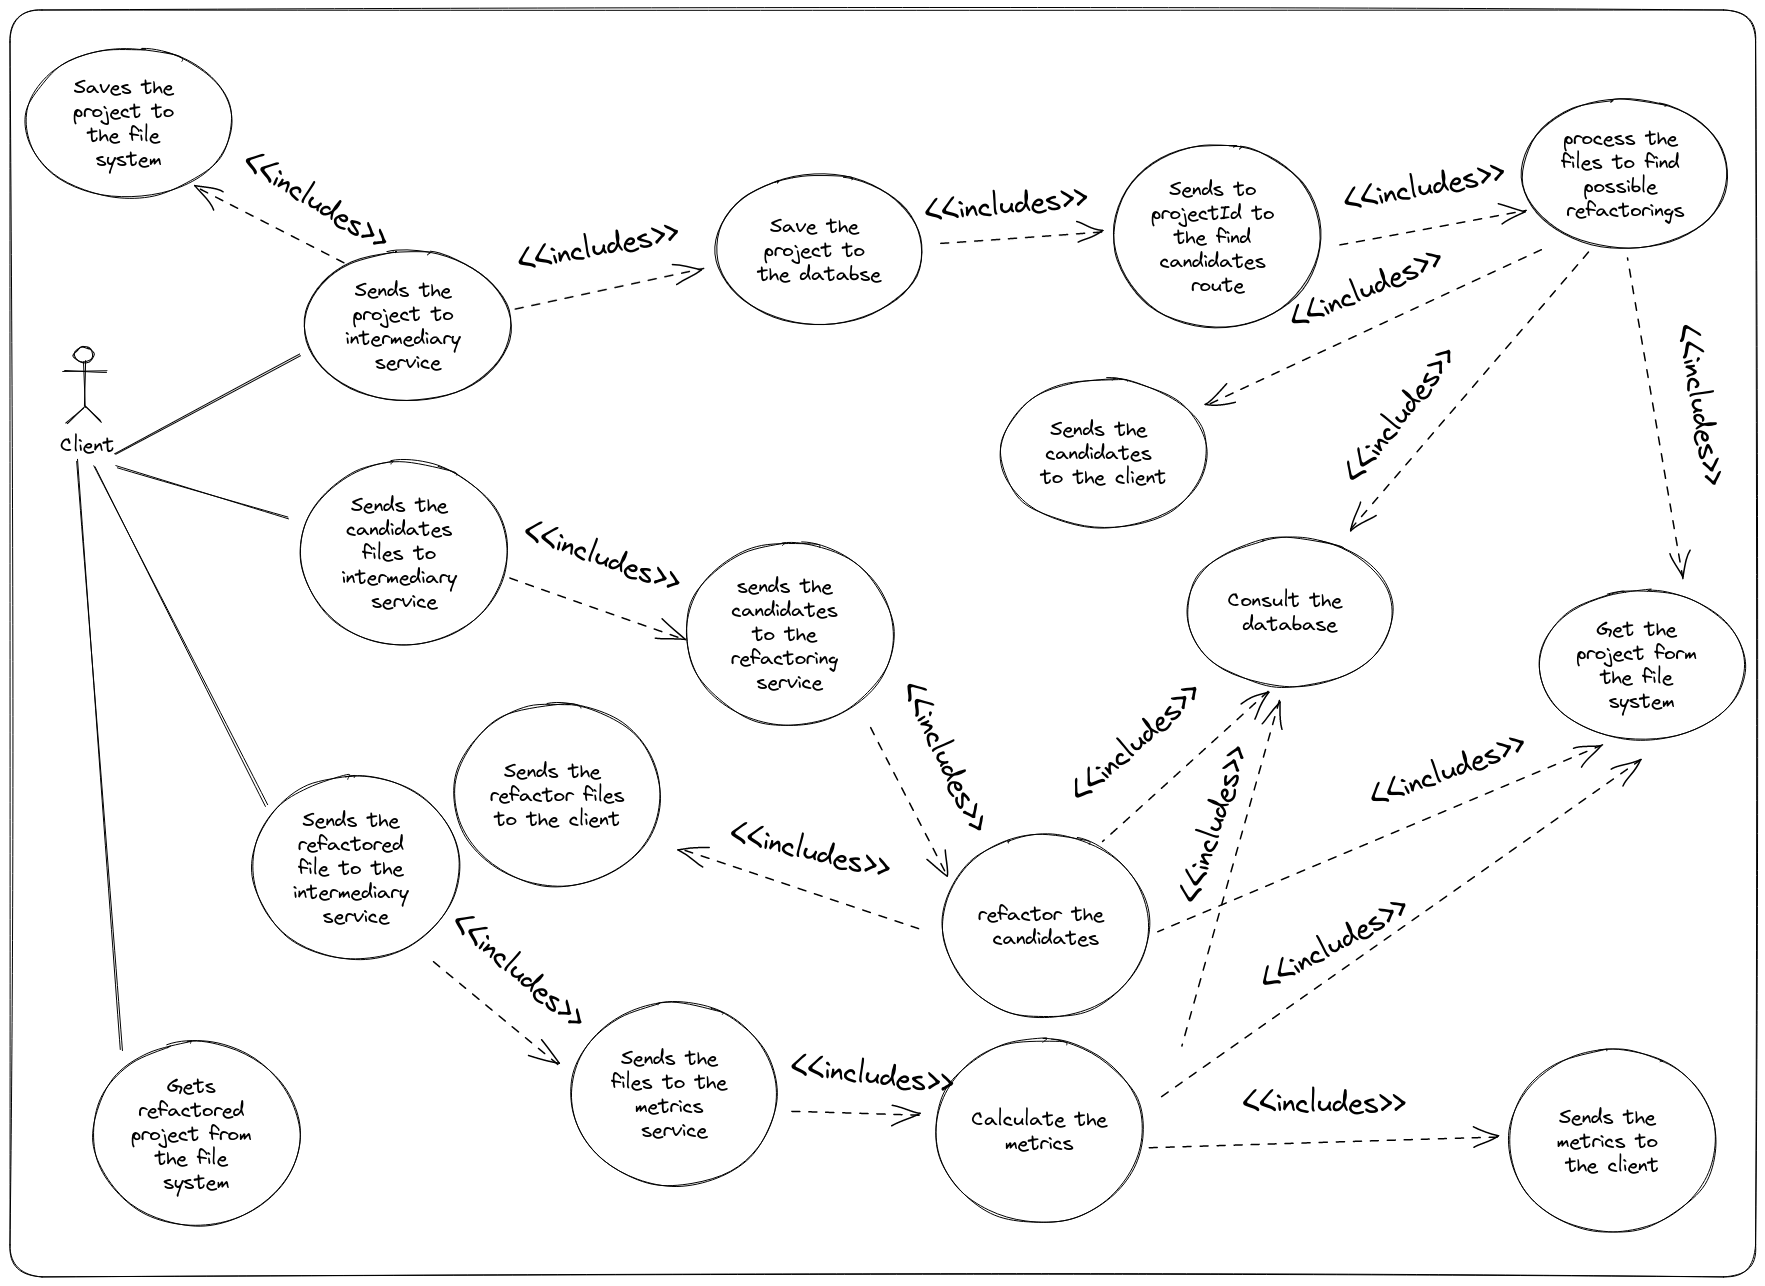
\includegraphics[width =\textwidth]{Chapter-2/Figures/usecase.png}
\SourceOrNote{Own authorship (2023)}
\end{figure}

The use case diagram describes the tool functionality for the user in \Cref{fig-usecase}; the client starts by uploading the project and searching for candidates; if any applicable method is found, the metric is calculated. On the interface, the client can select which class he wants to refactor, if any, and then refactor.


\subsubsection{RMT Architecture}
\label{sub-architecture}

 In addition to applying the refactorings, the tool uses the CK metrics extractor \cite{ck}, which encompasses the metrics of the depth of inheritance tree (PAH), cyclomatic complexity (CC), and program size in lines of code (TPLC). After selecting a project to be refactored, the metrics are applied to demonstrate the effects of refactorings on the user source code. The external quality attributes used were maintainability, reliability, and reusability.

The user iteration within the Client App can be performed independently since it communicates with the Intermediary Service, which provides the service that communicates the user layer (Client) with the processing layer (Services). The Intermediary Service uses a REST request for each service, one for the Metrics Service and one for the Detection Methods Service.

The model created by \textcite{beluzzo2018abordagem} also proposes a region's system structure with higher fault tolerance because the more Regions there are, the more members for processing will exist. Another factor \textcite{beluzzo2018abordagem} describes high availability, in which Regions should be placed on different servers, preventing overload and natural disasters. \Cref{fig-architecture} represents the regional divisions and application services.

\begin{figure}[ht!]
\SetCaptionWidth{\textwidth}
\caption{RMT architecture diagram}
\label{fig-architecture}
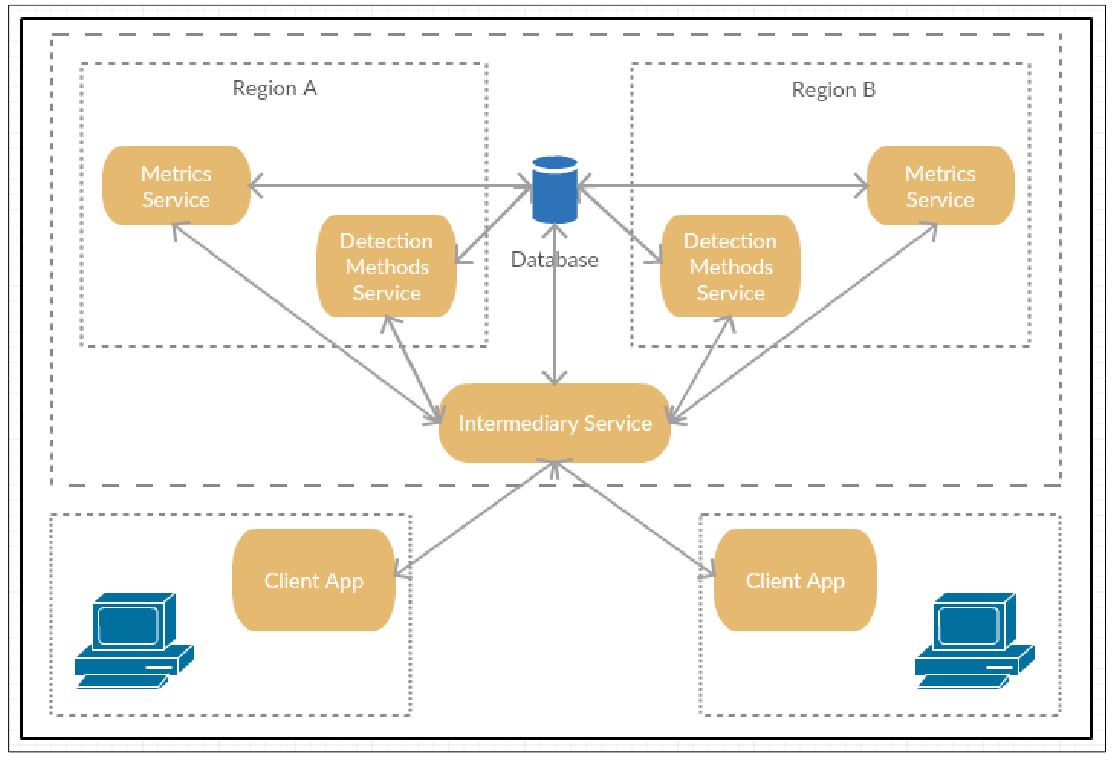
\includegraphics[width =\textwidth]{Chapter-2/Figures/schema.png}
\SourceOrNote{\textcite{beluzzo2018abordagem}}
\end{figure}


The architecture diagram in Figure 4 begins in the Client App. It continues to the Intermediary Service, which will choose the processing service depending on the user's action and may choose "Request source code evaluation" and "Request application of design patterns."
The Intermediary Service process, when it receives a refactoring candidate from the ClientApp, sends the request to the Intermediary service, which sends the request to the Detection Methods Service, which scans the database for source code and obtains the refactoring candidates. Then, the candidates are returned to the Intermediary service, which sends them to the Metrics Service for evaluation. 

After calculating the metrics, they are sent to the Intermediary service, which sends them back to the Client App to make the metrics and refactoring candidates available. If the user selects any refactoring candidates, the Client App sends the requests to the Intermediary Service with the candidates to be refactored in the Detection Methods Service. It creates a project with the refactorings performed.

\textcite{beluzzo2018abordagem} was concerned with abstracting the tool so that an expansion could be performed without significant problems, but he defined no extension process.

\subsubsection{Internal structure}
\label{subsub-internal}

A system's architecture is vital for working correctly, but all the heavy processing happens inside the services. A good design service will run with low memory and CPU, allowing it to work even in a small computer instance. The selection of refactoring candidates through RMT is described in \Cref{fig-candidates}.

\begin{figure}[ht!]
\SetCaptionWidth{\textwidth}
\caption{Sequence Diagram to Find Refactoring Candidates}
\label{fig-candidates}
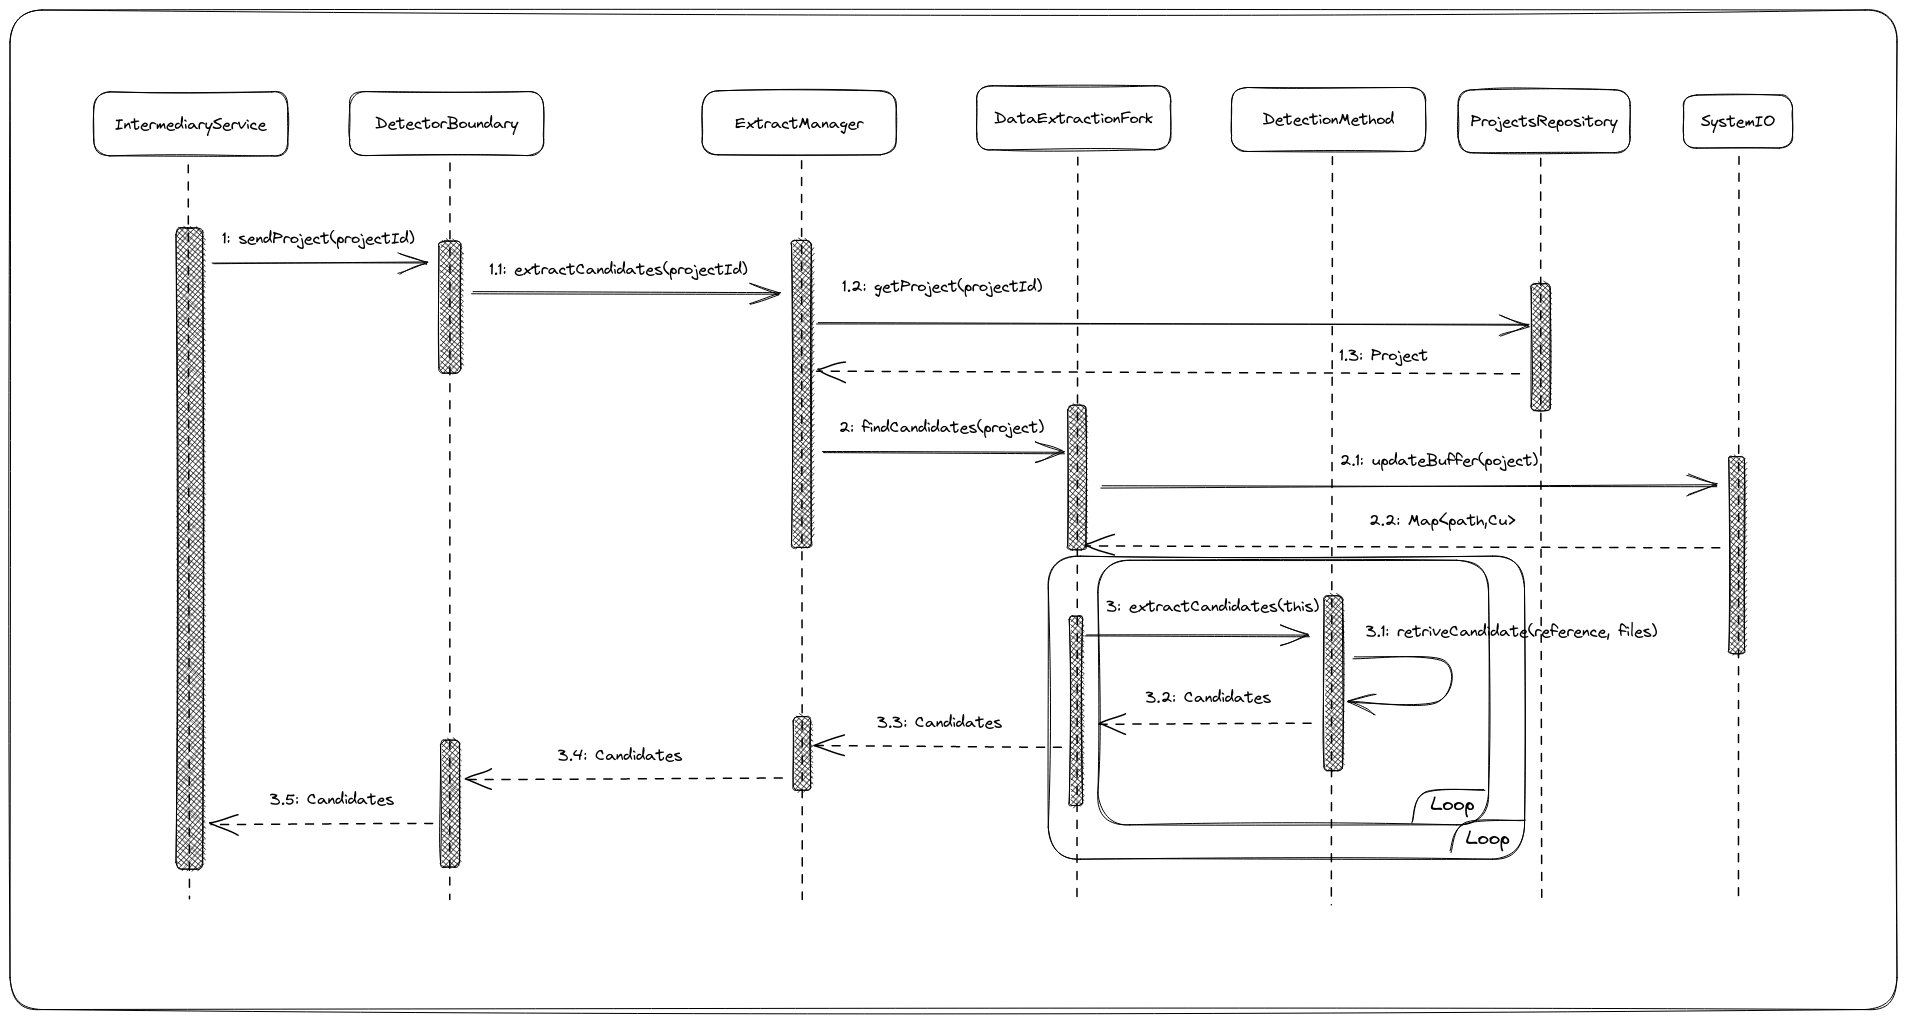
\includegraphics[width=160mm]{Chapter-2/Figures/candidates.png}
\SourceOrNote{Own authorship (2023)}
\end{figure}

As described in the architecture, the intermediary service communicates with the other services, which is why the diagram starts there. After saving the project path and ID to the database, the intermediary service sends the ID to the DetectionService as step 1.

On the detection service, the class to receive information is the DetectionBoundary, which gets the ID and passes it ahead as a simple controller in step 1.1. Step 2 sends the retrieved project to the DataExtractionFork.

The id is received by the ExtractManager, an interface responsible for retrieving the project from the project repository and sending it to be parsed on the DataExtractionFork as step 1.2.

The ProjectRepostiory is an interface with access to the database, which is consulted to retrieve the project information as a "Project" entity, completing step 1.3.

The DataExtractionFork has direct access to the system io, which is used to retrieve the project from the file system; the project is saved as a zip file inflated to be parsed as a CompilationUnit and loaded into the memory to be sent to every implementation of the DetectionMethod as step 2.1.

The DetectionMethod is an interface that abstracts the functionality of a new refactoring method; it receives an instance of the DataExtactionFork with the loaded files iterate over for every file and tries to detect if any pattern present on that method fits on the file and sends back the information via the stack finishing the step 3.1.

After the candidates' selection, if the user decides to refactor, the system sends the chosen files to the intermediary service, and the process described in \Cref{fig-refactoring} starts.

\begin{figure}[ht!]
\SetCaptionWidth{\textwidth}
\caption{Sequence Diagram for Refactoring Candidates}
\label{fig-refactoring}
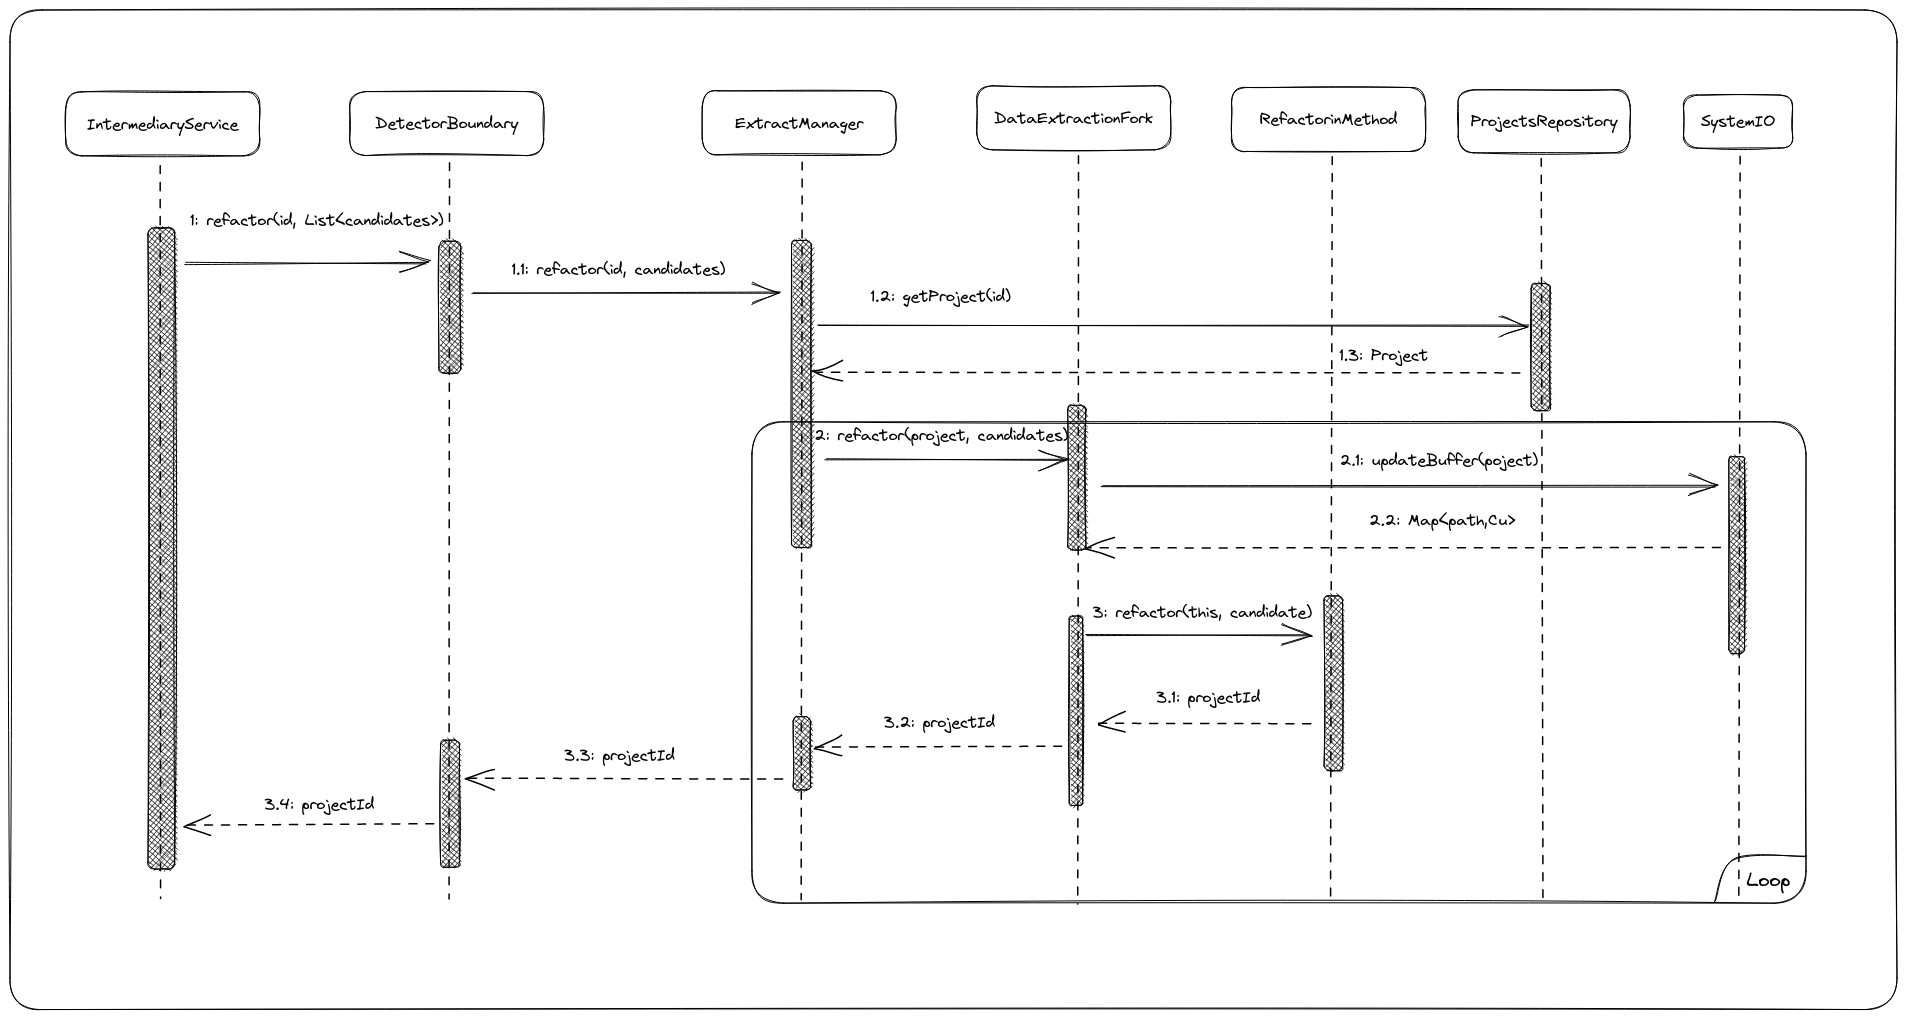
\includegraphics[width=160mm]{Chapter-2/Figures/refactoring.png}
\SourceOrNote{Own authorship (2023)}
\end{figure}


As the DetectionBoundry is the controller, it also revises the request to refactor with the user-selected classes and project ID to send to the ExtractManager as step 1.1.

The ExtractManager has the same functionality as on \Cref{fig-candidates}, retrieving the project from the database by the ProjectRepository (step 1.2) and sending iterating it to the DataExtractionFork as step 2.

The DataExtractionFrok in step 2.1 also has the same functionality. Still, every candidate on the project is called to return the same response every time, as it inflates the zip file and converts it to the CompilationUnit entity. For step 3, every candidate is sent to be refactored by the method defined on the candidate's face; after the process ends, the project ID is sent back via the stack.

\subsubsection{RMT Usage}
\label{sub-usage}

The main focus of explaining the usage of RMT is on the Client App, which is divided into three stages. The first step is importing the project, as shown in \Cref{fig-import}.

\begin{figure}[ht!]
\SetCaptionWidth{\textwidth}
\caption{Importing project on clientApp}
\label{fig-import}
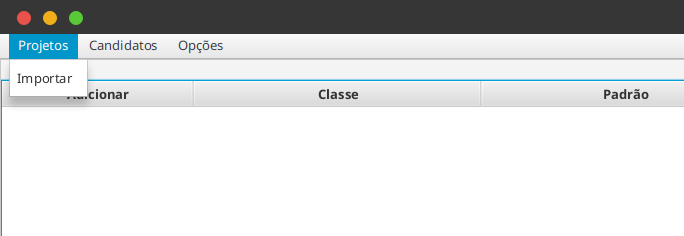
\includegraphics[width =100mm]{Chapter-2/Figures/import.png}
\SourceOrNote{Own authorship (2023)}
\end{figure}


The second step is the project evaluation, giving feedback to the user, which can analyze additional information about the refactoring candidates, such as class name, design pattern, and metrics, as shown in \Cref{fig-choose}.

\begin{figure}[ht!]
\SetCaptionWidth{\textwidth}
\caption{Selecting refactoring candidates}
\label{fig-choose}
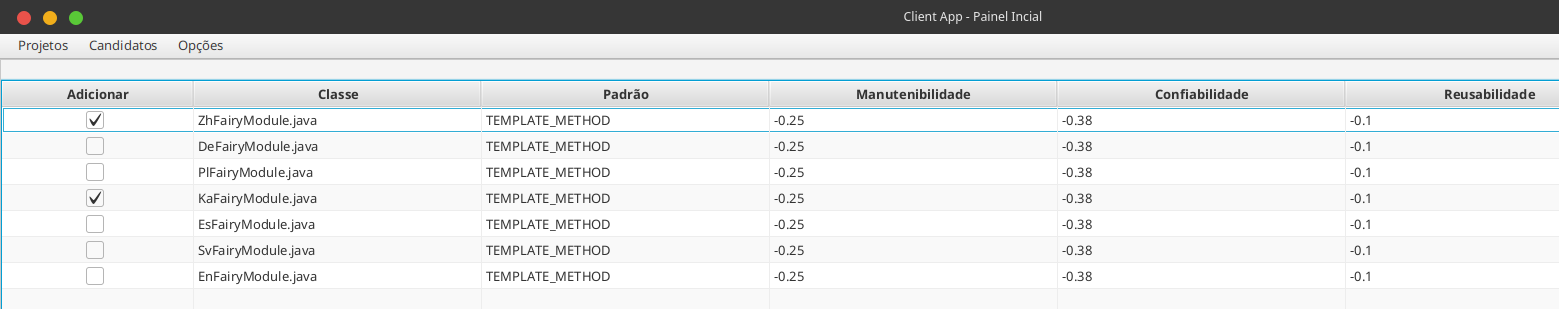
\includegraphics[width =\textwidth]{Chapter-2/Figures/choose.png}
\SourceOrNote{Own authorship (2023)}
\end{figure}

In the third and last step, the user can choose the candidates to apply the refactoring after using it to a new project created and saved in a directory selected by the user, as shown in \Cref{fig-refactor}.

\begin{figure}[ht!]
\SetCaptionWidth{\textwidth}
\caption{Applying refactoring to candidates}
\label{fig-refactor}
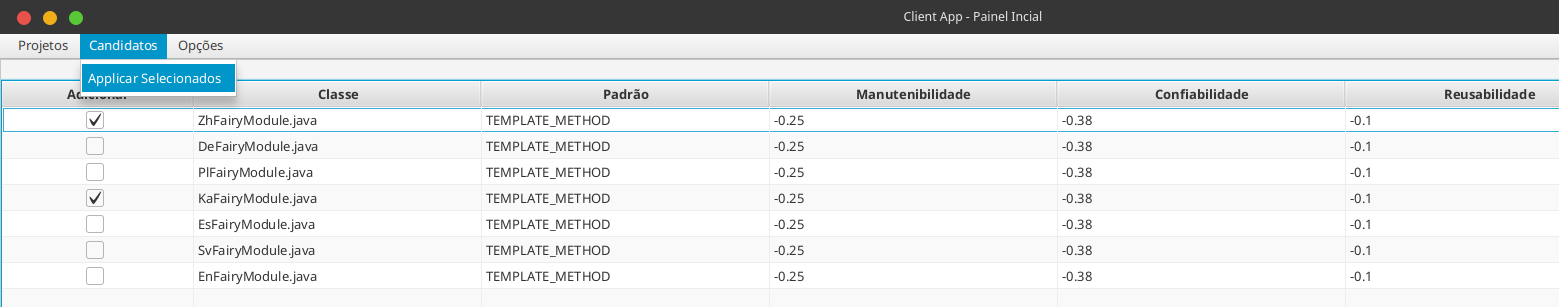
\includegraphics[width =\textwidth]{Chapter-2/Figures/refactor.png}
\SourceOrNote{Own authorship (2023)}
\end{figure}

\subsubsection{RMT Limitations}
\label{subsub-limitation}
When testing, the RMT can spot some limitations, such as the time to execute and a blocking request that may cause slowness when many users try to use the tool; also related to the slowness is that for every project, analyses and refactoring the system open a zip file and parses every file to memory to check if it's a candidate, and repeating the same process when it's refactoring the files, besides the fact that accessing the disk is takes time. For the interface, there is no explicit manner of choosing between the same pattern applied by two approaches in the same class.

The long time to execute is caused by the strategy of finding where the refactoring can be applied and the refactor action because it is synchronously performed on the same thread. Each file is analyzed in order, causing slowness on significant projects with many files.

The lack of performance happens when accessing the hard drive to retrieve the file for refactoring; for each refactoring step, the program parses the file and makes some changes to save it on disk; this could be solved by keeping the file in memory and changing it in memory.
The other problem implying the file system is that the architecture designed by \textcite{beluzzo2018abordagem} can be divided into regions, making it impossible to access the files with them being saved on one machine and the services being in another.

The blocking request is addressed when many users use the tool simultaneously, resulting in no more space for new connections. New users will increase latency, and users may receive an error and have to wait until someone refactors stops and opens space for a new connection. This problem mainly occurs because of the synchronous architecture on RMT based on an API composer (intermediary service) used to communicate with the other services via REST, providing dependency on the services as no intercommunication is made, acting as a load balancer, service registry, and discovery. The downside of REST communication is that the latency increases over the number of concurrent clients \cite{Cebeci2020DesignOA}. 

When RMT shows the patterns of refactoring candidates, it may show two refactoring for the same design pattern and class, having only the metrics to choose from which will be applied; it lacks other ways to explain the difference between the method to the user to make a better decision.

The tool is also missing unit tests, which could guarantee that the logic created in the class is correct and could help with the refactoring as it should not change the functionality, and the tests would have to continue working.

\section{Microservices Architecture}
\label{sec-microservices}
The microservices are used to create large and complex applications, as the model shown in \Cref{fig-architecture}, each application has to be simple and independent; when the services are connected and working together, they become a system. As discussed by \textcite{microservices-comuni}, the application is fault-tolerant and more controllable than a monolithic architecture.

There are many architectures, such as synchronous as RMT and asynchronous ones. The synchronous services wait for the response before ending the process; they usually use a direct connection over REST, RCP protocol, etc. \cite{microservices-comuni}. To implement a retry on sync services, the client service has to implement a strategy to handle the failure.

Asynchronous services do not wait for a response; the communication is non-block, so the service does not wait for the answer to end the process; it can be made with queues to handle communication. Those tools are RabbitMQ and Apache Kafka, among others \textcite{KARABEYAKSAKALLI2021111014}. Utilizing queues can bring new features related to resilience; if a service is down, the messages will be stored inside the queue and consumed when the service returns\cite{Cebeci2020DesignOA}. 

To work with retry, the queue has some implementations, such as visibility timeout, which is the time window in the message that is not visible to consumers; when the timeout is done and the message is not acknowledged, it becomes visible again, bringing resilience to the system, the downside is that it can duplicate the message over failure conditions \cite{ChenScalable}.

\section{Closing Remarks}
\label{sec2-remarks}
This chapter reported on the importance of refactoring, described the methods based on design patterns and refactoring tools, and explained some aspects of service architecture.

Refactoring is essential to keep the source code free of smells and to a quality standard. The main focus of refactoring is maintainability and reusability by maintaining the code as first designed and avoiding inserting new smells.

The importance of using a software refactoring tool was addressed to get the most out of refactoring without harming the work already done, emphasizing that the RMT tool is the focus of this research.
The RMT tool integrates several methods for detecting and inserting design patterns in a single environment so that the application developer can apply them in their source code without having to use several refactoring tools that have refactoring tools for this purpose.

There are many types of software architecture, but we discuss the abilities of the async and sync applications, bringing both upsides and downsides. As \textcite{beluzzo2018abordagem} did a systematic review to find papers on refactoring with design patterns and tools, another research method, such as snowballing, could be used to ensure that no other tool like RMT exists.

%% Capítulo 3
\chapter{State of Art}%
\label{chap-state}

Systematic literature review (SRL) studies are traditionally in software engineering, and software refactoring brings an excellent background for study analysis and classifications. As time passes, studies become obsolete as new articles are published monthly. A forward snowballing was proposed to update the systematic literature reviews on software refactoring.

This chapter is structured as \Cref{sec-background} describing the research methodology; \Cref{sec-methods} explaining the methods chosen to apply to the research; \Cref{sec-results} showing the results obtained in the study; \cref{sec-trends} explaining the trends in the research; \Cref{sec-cloasing-remarks} are the closing remarks.

\section{Background}
\label{sec-background}
According to \cite{bernard2006}, the snowballing technique is a non-probabilistic sampling technique that allows the reach of hard-to-reach or little-known populations. It occurs due to its mechanism of establishing a network of relationships among the elements, creating a chain of references.

The technique has three objectives: to improve the understanding of a theme, verify the possibility of conducting a more extensive study, and develop methods to be employed in subsequent studies and phases \cite{vinuto2014}. Snowballing is used mainly for experimental purposes.

The procedure for following the Snowballing technique is described in the following steps: start set, iterations (backward snowballing, forward snowballing, and inclusion and exclusion), identification of the authors, and data extraction \cite{Wohlin2014}.

The first step of snowballing is creating a starting set of papers; a viable option is to use search engines such as Google Scholar. It is an excellent alternative to avoid bias in favor of any author \cite{Wohlin2014}.

\textcite{Kitchenham2013} chose a set of works to start the snowballing; they preferred to use two conference proceedings, the Evaluation and Assessment in Software Engineering and Empirical Software Engineering and Measurement Searching, from 2005 to mid-2012. We chose first to utilize a database search with a string and search engines as it avoids the bias of a starter set of SRL before the forward snowballing to update the fancied SLR.

The title and abstract are the elements to consider when selecting suitable candidate papers. The main goal is to avoid unrelated works, but only if they are explicitly irrelevant, and the premise is to include any paper that may be relevant. To select or remove articles, all authors must agree, and if there is any estrangement, discussions may occur until their consent is defined \textcite{Kitchenham2013}.

After establishing the initial set, the iteration step is performed by performing Backward Snowballing and Forward Snowballing, including and excluding new jobs in the collection \cite{Wohlin2014}.

Backward snowballing consists of using the list of references to identify new articles to be analyzed later on. The first step is to review the references and discard the papers that do not meet the essential research criteria. The second step is to remove the reports that have already been examined from the list. The first two steps are about extracting information from the article, and a new article should not be studied if there is not enough information in the analyzed document \cite{Wohlin2014}.

Conversely, forward snowballing consists of using the list of citations to identify new articles to be analyzed later. The first step is to review the citations in an online database and discard papers that do not meet the essential criteria. The following steps follow the same concept as forward-backward snowballing \cite{Felizardo2016}.

\section{Methods}
\label{sec-methods}
Database searches were used to start a systematic literature review update. For instance, to find a search string, the databases were chosen to search for and determine the exclusion and inclusion to decide which of the found studies are adequate to enter as a starter set for the forward snowballing.

It is challenging to assemble a suitable string, as the terminology used in software engineering is not standardized. Using a specific keyword may find a few relevant articles and even miss some suitable works; otherwise, using generic keywords may result in irrelevant articles, creating unnecessary labor \cite{Wohlin2014}.

To find the starter set of SLR to apply the forward snowballing, a database search with a specific set of keywords was determined, and the found collection of papers will be updated as a result of the process. The search string to initiate the snowballing approach is (("systematic literature review") OR ("systematic review") OR ("systematic mapping review") OR ("systematic mapping") ) AND "software refactoring" and includes all the main desired topics to search, such as SLR and systematic mapping review (SMR) with two options keywords for each to result in a more accurate search on the subject. An inclusion and exclusion criteria list was defined to select the papers returned by the search string.

The inclusion criteria are as follows:

\begin{itemize}
    \item The publishing year of the articles must be between 1992 and 2022, as \textcite{Opdyke1992} was the first person to publish with the refactoring term;
    \item Systematic literature review articles and systematic mapping reviews about software refactoring methods, frameworks, technics; or applications or development, methods or practices code smells detections;
\end{itemize}

The criteria for exclusions are as follows.

\begin{itemize}
    \item Article not written in English or Portuguese;
    \item Non-source code studies or architecture refactoring;
    \item Abstract, posters, patents, and keynotes;
\end{itemize}

The standards must be followed by reading the article's title to filter the studies using the above criteria. If it already has the information to be accepted, no more reading is necessary for inclusion; if only the title is insufficient, the abstract is thoroughly read to understand more about the paper's objectives. The whole article is read if there is still doubt about the exclusion or inclusion. \textcite{Wohlin2014} does not recommend reading the report from the beginning; instead, he argues that it is best to read the most relevant parts to make a decision.
The search engines were Google Scholar, Springer, Science Direct, ResearchGate, IEEE Xplore, and ACM. From these bases, 804 articles were divided per database: 689 from Google Scholar, 43 from Springer, 32 from Science Direct, 25 from ResearchGate, 12 from ACM, and three from IEEE Xplore, as shown in \Cref{tab-reviews}.

To apply forward snowballing, Google Scholar was chosen to look for citations, as it is an excellent way to avoid bias \cite{Wohlin2014}. All articles were subjected to one interaction with the original SRL as sed set, evidenced by \textcite{Wohlin2020} as the most cost-effective approach to update the studies. The diagram in \Cref{fig-snow} exemplifies the whole search method. 

\begin{figure}[ht!]
\SetCaptionWidth{\textwidth}
\caption{Search Method Diagram}
\label{fig-snow}
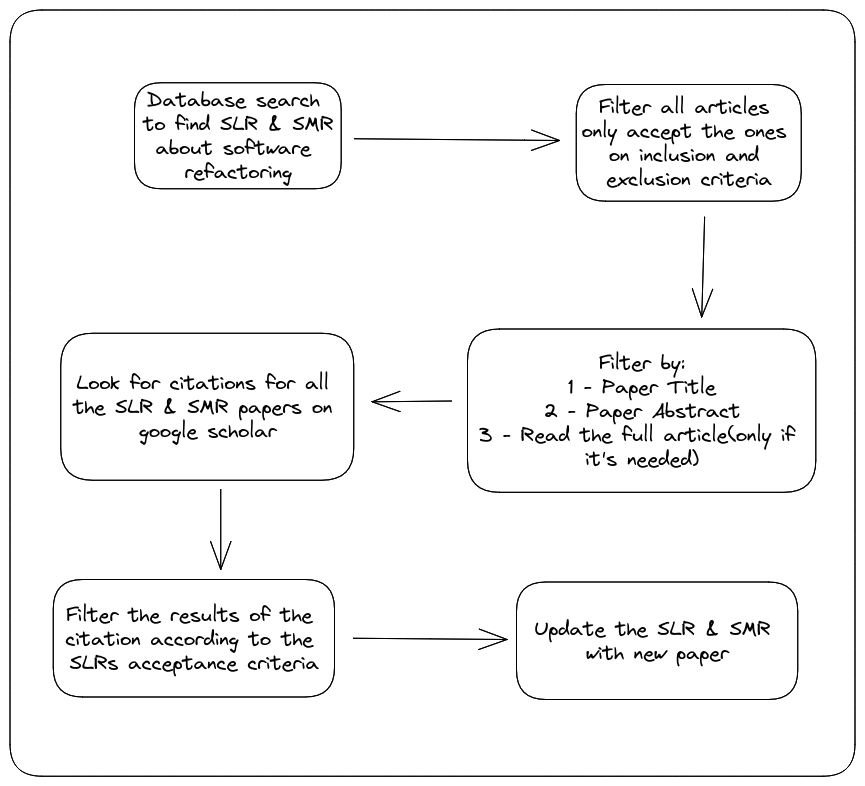
\includegraphics[width =100mm]{Chapter-3/Figures/snowballing_diagram.png}
\SourceOrNote{Own authorship (2023)}
\end{figure}
\FloatBarrier

As in the database search, snowballing inclusion and exclusion criteria must be applied in the papers that have cited the current SRL. The requirements must come from the starting set of documents \cite{Wohlin2020}. Reading every SRL, it generally finds a section explaining those accepted standards.


\section{Results}
\label{sec-results}
\Cref{tab-reviews} shows all the papers found on the database search to achieve the start set for snowballing; it contains an id composed of S representing the start and a number. The table is sorted by title and contains the total number of citations found in Google Scholar for each article and the reference.

\begin{tabframed}
\caption{Select papers from database search}
\label{tab-reviews}
\begin{tabularx}{\textwidth}{|e{}@{},{}@{}|p{9cm}|c|p{3cm}@{}|}
\toprule%
\multicolumn{1}{|@{}c|}{\textbf{Key}}        &
\multicolumn{1}{c|}{\textbf{Tile}}    &
\multicolumn{1}{c|}{\textbf{Citation  Nº}}  &
\multicolumn{1}{c@{}|}{\textbf{Ref}}        \\
\midrule% 
S1  & 30 Years of Software Refactoring Research:A Systematic Literature Review                           & 13          & \citeauthor*{Abid2020}                               \\
S2  & A Literature Review on Code Smells and Refactoring                                                 & 17          & \citeauthor*{Ruben2010}                              \\
S3  & A Systematic Literature Review on Software Refactoring                                             & 0           & \citeauthor*{Elhazzat2020}                           \\
S4  & A Systematic Literature Review on Software-refactoring Techniques, Challenges, and Practices       & 0           & \citeauthor*{Akhtar2022}                             \\
S5  & A systematic literature review: Refactoring for disclosing code smells in object oriented software & 74          & \citeauthor*{Singh2018b}                              \\
S6  & A systematic literature survey of software metrics, code smells and refactoring techniques         & 15          & \citeauthor*{Agnihotri2020}                          \\
S7  & A systematic mapping of literature on software refactoring tools                                   & 3           & \citeauthor*{Tavares2018}                            \\
S8  & A systematic review on search-based refactoring                                                    & 78          & \citeauthor*{Mariani2017}                            \\
S9  & Automatic software refactoring: a systematic literature review                                     & 40          & \citeauthor*{Baqais2020}                             \\
S10 & Classification and Summarization of Software Refactoring Researches: A Literature Review Approach  & 4           & \citeauthor*{Abebe2014b}                              \\
S11 & Code Smells and Refactoring: A Tertiary Systematic Review of Challenges and Observations           & 47          & \citeauthor*{Lacerda2020}                            \\
S12 & Multi-Objective Optimization Techniques for Software Refactoring: A Systematic Literature Review   & 1           & \citeauthor*{Rafique2019}                            \\
S13 & On preserving the behavior in software refactoring: A systematic mapping study                     & 15          & \citeauthor*{AlOmar2021}                             \\
S14 & Trends, opportunities and challenges of software refactoring: A systematic literature review       & 42          & \citeauthor*{Abebe2014a}                              \\
S15 & Why , How , and When Refactorings are ( NOT ) Applied : A Systematic Literature Review             & 0           & \citeauthor*{Buriakovskyi2018}                                \\
\bottomrule%
\end{tabularx}
\SourceOrNote{Own authorship (2023)}           
\end{tabframed}
\FloatBarrier

The most crucial part of updating the SRLs in the acceptance criteria is that their interpretation will decide if a cited paper has the qualities to be included in its update. Most studies have an explicit acceptance criterion besides S3, S7, S10, and S12. Although S12 has no detailed parameters, the questions are well-defined enough to use as a selection method for snowballing; unfortunately, the paper has no citations. For S10, the criteria to include in the update were the classification made from the SLR-selected articles. However, finding an alternative to filter the citations became less secure in fitting the original article because the author did not have a particular sentiment. 

Multiple articles did not include some styles of publications, such as abstracts, posters, and keynotes for S8, S9, and S13, gray literature for S1, S8, and S9, doctoral symposiums, books, and theses for S8 and S9. In the gray literature, it may not be the most reasonable guideline to follow because, as shown in articles S1 and S11, the first time worked with the term refactoring was in 1992 by \textcite{Opdyke1992}, which was a Ph.D. thesis. According to \textcite{Buriakovskyi2018}, only after the published book \textcite{fowler2018refactoring} did the active research on the practical use of refactoring begin. This would exclude both studies from S8 and S9.

The number of studies selected and filtered for each article was quite different; after removing duplicates, the final result was six articles for S1, 4 for S2, 13 for S5, 4 for S6, 16 for S8, 5 for S9, 1 for S10, 15 for S11, and 1 for S13. Sixty-five possible papers will be included in future SLR updates as the analyses cover each article's approval criteria.

 \Cref{tab-snow} shows all the selected papers from applying the forward snowballing and following the acceptance criterion from all the SLRs. The first row has the ID studies from the starter set referenced; the cited papers ID is in n the second column referenced with the SLR ID and a capital C and a number; the title is in the third column, and the bibliographic reference is in the last column.

\begin{longtable}{|e{}@{},{}@{}|c|p{9cm}|p{3cm}@{}|}
%% Cabeçalho da primeira página
\caption{Resultant Articles with design patterns methods}
\label{tab-snow}                                              \\[\belowcaptionskip]
\multicolumn{4}{@{}r@{}}{\textbf{(continue)}}                 \\[\belowcaptionskip]
\toprule%
\multicolumn{1}{|@{}c|}{\textbf{Key}}        &
\multicolumn{1}{c|}{\textbf{Id}}            &
\multicolumn{1}{c|}{\textbf{Title}}         &
\multicolumn{1}{c@{}|}{\textbf{Ref}}        \\
\midrule%
\endfirsthead%
%% Cabeçalho das páginas (exceto primeira e última)
\caption[]{Resultant Articles with design patterns methods}   \\[\belowcaptionskip]
\multicolumn{4}{@{}r@{}}{\textbf{(continuation)}}             \\[\belowcaptionskip]
\toprule%
\multicolumn{1}{|@{}c|}{\textbf{Key}}        &
\multicolumn{1}{c|}{\textbf{Id}}            &
\multicolumn{1}{c|}{\textbf{Title}}         &
\multicolumn{1}{c@{}|}{\textbf{Ref}}        \\
\midrule%
\endhead%
%% Cabeçalho da última página
\caption[]{Resultant Articles with design patterns methods}   \\[\belowcaptionskip]
\multicolumn{4}{@{}r@{}}{\textbf{(conclusion)}}               \\[\belowcaptionskip]
\toprule%
\multicolumn{1}{|@{}c|}{\textbf{Key}}        &
\multicolumn{1}{c|}{\textbf{Id}}            &
\multicolumn{1}{c|}{\textbf{Title}}         &
\multicolumn{1}{c@{}|}{\textbf{Ref}}        \\
\midrule%
\endlasthead%
%% Rodapé da última página
\bottomrule%
\LTSourceOrNote{Own authorship (2023)}           \\
\endlastfoot% 

S1  &        &                                                                                                                                                                                                                                               &                                 \\
    & S1-C1   & Generation of refactoring algorithms by grammatical evolution                                                                                                                                                                                  & \citeauthor*{Mariani2022}     \\
    & S1-C2   & Refactorings and Technical Debt in Docker Projects: An Empirical Study                                                                                                                                                                         & \citeauthor*{Ksontini2021}    \\
    & S1-C3   & RefDetect: A Multi-Language Refactoring Detection Tool Based on String Alignment                                                                                                                                                               & \citeauthor*{Moghadam2021}    \\
    & S1-C4   & Supporting refactoring of BDD specifications—An empirical study                                                                                                                                                                                & \citeauthor*{Irshad2022}      \\
    & S1-C5   & Refactoring Techniques for Improving Software Quality: Practitioners’ Perspectives                                                                                                                                                             & \citeauthor*{Ksontini2021}    \\
    & S1-C6   & Automated refactoring of legacy JavaScript code to ES6 modules                                                                                                                                                                                 & \citeauthor*{Paltoglou2021}   \\
S2  &        &                                                                                                                                                                                                                                               &                                 \\
    & S2-C1   & Design and Implementation of a Web-Based Application for Code Smells Repository                                                                                                                                                                & \citeauthor*{Bamizadeh2021}   \\
    & S2-C2   & Object-Oriented Code Metric-Based Refactoring Opportunities Identification Approaches: Analysis                                                                                                                                                & \citeauthor*{Bassey2017}      \\
    & S2-C3   & Analysing The Effects Of Refactoring On Software Quality Attributes                                                                                                                                                                            & \citeauthor*{Singh2018a}       \\
    & S2-C4   & Measuring Code Smells and Anti-Patterns                                                                                                                                                                                                        & \citeauthor*{Reeshti2019}     \\
S5  &        &                                                                                                                                                                                                                                               &                                 \\
    & S5-C1   & Code Smell Refactoring for Energy Optimization of Android Apps                                                                                                                                                                                 & \citeauthor*{Reeshti2021}     \\
    & S5-C2   & Software Engineering Paradigm for Real-Time Accurate Decision Making for Code Smell Prioritization                                                                                                                                             & \citeauthor*{Singh2021}       \\
    & S5-C3   & A Framework to Improve Quality of a Java System by Performing Refactoring                                                                                                                                                                      & \citeauthor*{singhAndBindal2020}       \\
    & S5-C4   & Detecting Sudden Variations in Web Apps Code Smells’ Density: A Longitudinal Study                                                                                                                                                             & \citeauthor*{Rio2021}         \\
    & S5-C5   & Controlling software evolution process using code smell visualization                                                                                                                                                                          & \citeauthor*{Nabilah2019}     \\
    & S5-C6   & PHP code smells in web apps: survival and anomalies                                                                                                                                                                                            & \citeauthor*{Rio2021}         \\
    & S5-C7   & Bad Smell Detection Using Machine Learning Techniques: A Systematic Literature Review                                                                                                                                                          & \citeauthor*{Al-Shaaby2020}   \\
    & S5-C8   & Recovering Android Bad Smells from Android Applications                                                                                                                                                                                        & \citeauthor*{Rasool2020}      \\
    & S5-C9   & To improve code structure by identifying move method opportunities using frequent usage patterns in source-code                                                                                                                                & \citeauthor*{Singh2019}       \\
    & S5-C10  & Using software metrics to detect temporary field code smell                                                                                                                                                                                    & \citeauthor*{Gupta2020a}      \\
    & S5-C11  & Rank-based univariate feature selection methods on machine learning classifiers for code smell detection                                                                                                                                       & \citeauthor*{Jain2022}        \\
    & S5-C12  & TFfinder: A Software tool to discover Temporary Field code smell                                                                                                                                                                               & \citeauthor*{Gupta2020b}      \\
    & S5-C13  & Analysis of code smell to quantify the refactoring                                                                                                                                                                                             & \citeauthor*{Sehgal2017}      \\
S6  &        &                                                                                                                                                                                                                                               &                                 \\
    & S6-C1   & Does Code Complexity Affect the Quality of Real-Time Projects?: Detection of Code Smell on Software Projects using Machine Learning Algorithms                                                                                                 & \citeauthor*{Patnaik2021b}    \\
    & S6-C2   & A hybrid approach to identify code smell using machine learning algorithms                                                                                                                                                                     & \citeauthor*{Patnaik2021a}     \\
    & S6-C3   & Illustration and detection of exception handling bad smells                                                                                                                                                                                    & \citeauthor*{Tarwani2021}     \\
    & S6-C4   & Automated refactoring of legacy JavaScript code to ES6 modules                                                                                                                                                                                 & \citeauthor*{Paltoglou2021}   \\
S8  &        &                                                                                                                                                                                                                                               &                                 \\
    & S8-C1   & Enabling Decision and Objective Space Exploration for Interactive Multi-Objective Refactoring                                                                                                                                                  & \citeauthor*{Rebai2020}       \\
    & S8-C2   & Explainable Search-Based Refactoring                                                                                                                                                                                                           & \citeauthor*{Abid2021c}       \\
    & S8-C3   & Intelligent Change Operators for Multi-Objective Refactoring                                                                                                                                                                                   & \citeauthor*{Abid2021a}       \\
    & S8-C4   & Interactive Decision and Objective Space Exploration for Search Based Refactoring                                                                                                                                                              & \citeauthor*{Rebai2019}       \\
    & S8-C5   & A Many-Objective Estimation Distributed Algorithm Applied to Search Based Software Refactoring                                                                                                                                                 & \citeauthor*{Botelho2018}     \\
    & S8-C6   & X-SBR: On the Use of the History of Refactorings for Explainable Search-Based Refactoring and Intelligent Change Operators                                                                                                                     & \citeauthor*{Abid2021b}       \\
    & S8-C7   & The Effectiveness of Supervised Machine Learning Algorithms in Predicting Software Refactoring                                                                                                                                                 & \citeauthor*{Aniche2022}      \\
    & S8-C8   & Improving Readability of Scratch Programs with Search-based Refactoring                                                                                                                                                                        & \citeauthor*{Adler2021}       \\
    & S8-C9   & Untangling the Knot: Enabling Architecture Evolution with Search-Based Refactoring                                                                                                                                                             & \citeauthor*{Ivers2022}       \\
    & S8-C10  & Harnessing deep learning algorithms to predict software refactoring                                                                                                                                                                            & \citeauthor*{Alenezi2020}     \\
    & S8-C11  & DEPICTER: A Design-Principle Guided and Heuristic-Rule Constrained Software Refactoring Approach                                                                                                                                               & \citeauthor*{Zhao2022}        \\
    & S8-C12  & EASIER: An Evolutionary Approach for Multi-objective Software ArchItecturE Refactoring                                                                                                                                                         & \citeauthor*{Arcelli2018}     \\
    & S8-C13  & Unsupervised Learning For Refactoring Pattern Detection                                                                                                                                                                                        & \citeauthor*{Farah2021}       \\
    & S8-C14  & Model refactoring by example: A multi-objective search based software engineering approach                                                                                                                                                     & \citeauthor*{Ghannem2018}     \\
    & S8-C15  & A survey of many-objective optimisation in search-based software engineering                                                                                                                                                                   & \citeauthor*{Ramirez2019}     \\
    & S8-C16  & Applying design patterns in the search-based optimization of software product line architectures                                                                                                                                               & \citeauthor*{Guizzo2019}      \\
S9  &        &                                                                                                                                                                                                                                               &                                 \\
    & S9-C1   & An automated extract method refactoring approach to correct the long method code smell                                                                                                                                                         & \citeauthor*{Shahidi2022}     \\
    & S9-C2   & Automated Refactoring of Unbounded Queries in Software Automation Platforms                                                                                                                                                                    & \citeauthor*{Fernandes2021}   \\
    & S9-C3   & Cross-Project Software Refactoring Prediction Using Optimized Deep Learning Neural Network With the Aid of Attribute Selection                                                                                                                 & \citeauthor*{Panighrahi2022}  \\
    & S9-C4   & An automatic refactoring framework for replacing test-production inheritance by mocking mechanism                                                                                                                                              & \citeauthor*{Wang2021}        \\
    & S9-C5   & Refactoring Legacy Software for Layer Separation                                                                                                                                                                                               & \citeauthor*{Khalilipour2021} \\
S10 &        &                                                                                                                                                                                                                                               &                                 \\
    & S10-C1  & Composite Refactoring: Representations, Characteristics and Effects on Software Projects                                                                                                                                                       & \citeauthor*{Bibiano2022}     \\
S11 &        &                                                                                                                                                                                                                                               &                                 \\
    & S11-C1  & RefDiff4Go: Detecting Refactorings in Go                                                                                                                                                                                                       & \citeauthor*{Brito2020}       \\
    & S11-C2  & Test smell detection tools: A systematic mapping study                                                                                                                                                                                         & \citeauthor*{Aljedaani2021}   \\
    & S11-C3  & An automated extract method refactoring approach to correct the long method code smell                                                                                                                                                         & \citeauthor*{Shahidi2022}     \\
    & S11-C4  & Automated refactoring of legacy JavaScript code to ES6 modules                                                                                                                                                                                 & \citeauthor*{Paltoglou2021}   \\
    & S11-C5  & Automatic detection of Long Method and God Class code smells through neural source code embeddings                                                                                                                                             & \citeauthor*{Kovačević2022}   \\
    & S11-C6  & Are Code Smell Co-occurrences Harmful to Internal Quality Attributes?: A Mixed-Method Study                                                                                                                                                    & \citeauthor*{Martins2020}     \\
    & S11-C7  & How do Code Smell Co-occurrences Removal Impact Internal Quality Attributes? A Developers' Perspective                                                                                                                                         & \citeauthor*{Martins2021}     \\
    & S11-C8  & "Project smells" -- Experiences in Analysing the Software Quality of ML Projects with mllint                                                                                                                                                   & \citeauthor*{van2022}         \\
    & S11-C9  & Toward the automatic classification of Self-Affirmed Refactoring                                                                                                                                                                               & \citeauthor*{AlOmar2021b}     \\
    & S11-C10 & A framework to improve quality of a Java system by performing refactoring Currently I am working on Disaster Management and energy efficient deployment View project A framework to improve quality of a Java system by performing refactoring & \citeauthor*{Singh2020}       \\
    & S11-C11 & TERTIARY STUDY on LANDSCAPING the REVIEW in CODE SMELLS                                                                                                                                                                                        & \citeauthor*{Yaqoob2021}      \\
    & S11-C12 & MARS: Detecting brain class/method code smell based on metric–attention mechanism and residual network                                                                                                                                         & \citeauthor*{Zhang2021a}       \\
    & S11-C13 & RAID: Tool Support for Refactoring-Aware Code Reviews                                                                                                                                                                                          & \citeauthor*{Brito2021}       \\
    & S11-C14 & Code smells detection and visualization: A systematic literature review                                                                                                                                                                        & \citeauthor*{Pereira2022}     \\
S13 &        &                                                                                                                                                                                                                                               &                                 \\
    & S13-C1  & Consistency validation method for Java fine-grained lock refactoring                                                                                                                                                                           & \citeauthor*{Zhang2021b}         
\end{longtable}
\FloatBarrier

It was possible to analyze that some papers cited more than one SLR with slightly different subjects but the same refactoring matter. The article by \textcite{Paltoglou2021} focuses on proposing refactoring legacy Javascript to a newer version called ES6 with many more features and reliability. The study appears on S1, S6, and S11.


\section{Trends}
\label{sec-trends}
This study used forward snowballing to propose a set of papers to be candidates for its original SRLs and SMRs.
A total of 65 papers could be included in their respective SRLs as the final step of the snowballing, considering the acceptance criteria of the original papers, which strictly ensures quality. In conclusion, snowballing showed an excellent and fast way to update an SRL and SMR.
The paper also shows how SLRs can age pretty well, like S9, a work from 2020 that already has 40 citations, where, after filtering, five possible studies were achieved to include in an update of this paper.

As argued, SRLs age quite rapidly; the same will happen with work as new papers are published every month, and some of those are likely to cite an article from the starter set, assuming that to avoid paper aging, they ought to apply an update of the database search and snowballing in a fixed data frame.

\section{Closing Remarks}
\label{sec-cloasing-remarks}

The main application of snowballing in this work is to find new methods to find opportunities to refactor Java code to apply design patterns by finding all refactoring-related SLRs and SMRs and applying the snowballing techniques. After the process, no new article was found on the desired topic. That shows the importance of RMT and how a tool that can concentrate all refactoring methods to design patterns has not yet been found in the academy and can change how developers apply refactorings to their projects.

%% Capítulo 4
\chapter{Methodology used to refactor and improve RMT tool}%
\label{methodology}

This chapter explores the methodology for refactoring and improving the RMT tool. It delves into various techniques and best practices for improving and optimizing the tool's performance and maintainability. The discussion covers a range of refactoring strategies.

The methodology is delineated into five sequentially interconnected phases as depicted in \cref{fig-overview-methodology}. Each phase systematically uses the insights and understanding obtained from the previous stage to optimize its efficacy. 

\begin{figure}[ht!]
\SetCaptionWidth{\textwidth}
\caption{Methodology Overview Diagram}
\label{fig-overview-methodology}
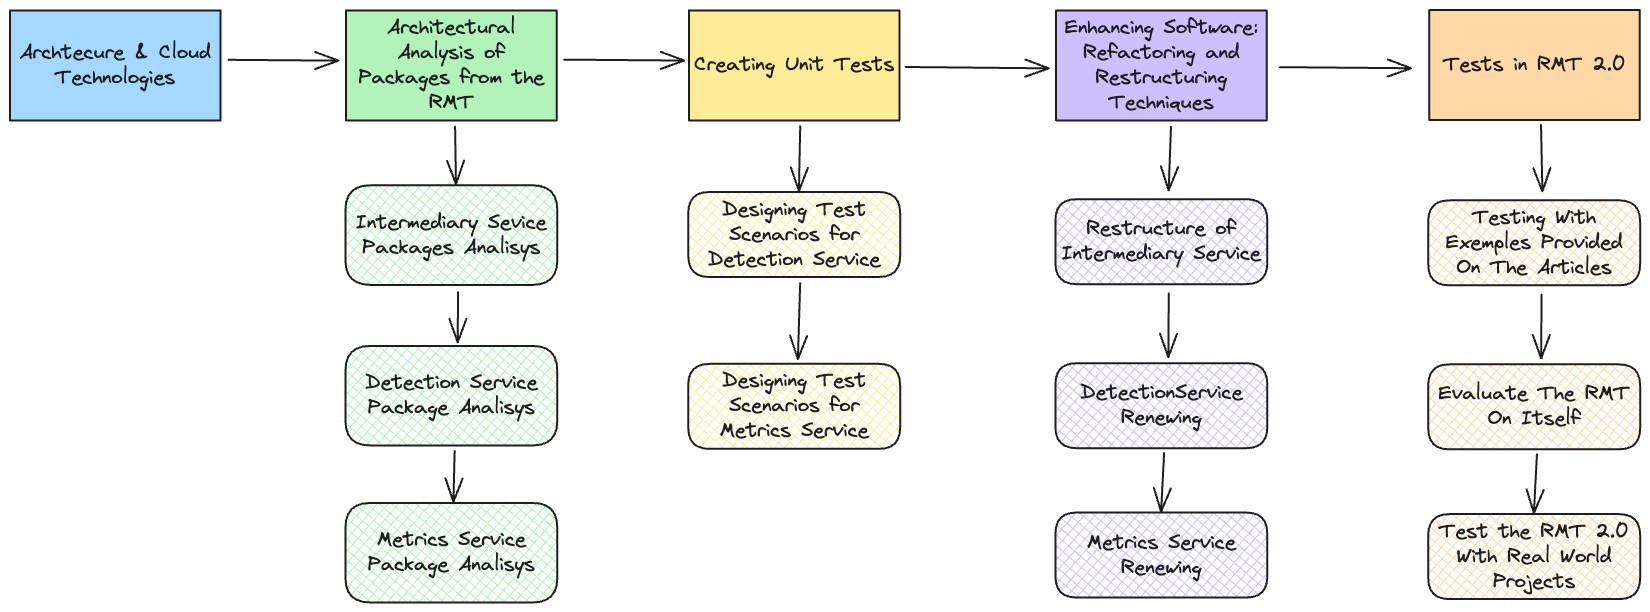
\includegraphics[width =\textwidth]{Chapter-4/Figures/Metodologia.png}
\SourceOrNote{Own authorship (2024)}
\end{figure}
\FloatBarrier


Each phase of the methodology is described in the clauses of this chapter. The \cref{sec-arch-cloud} explores the methodology through cloud technologies. The \cref{sec-archtectural-analysis}, \ref{sub-intermediary-packages}, \ref{sub-detection-packages}, and \ref{sub-metrics-packages} explain the analytic processes used to formulate strategic modifications to the codebase and delineate the functionalities of each package within the services. The \cref{sec-creating-tests}, \ref{detection-design-tests}, and \ref{metrics-design-tests} elaborate on the comprehensive testing procedures for each service, detailing the criteria for selecting tested classes. The \cref{sec-enhancing}, \ref{sub-restruct-intermediary}, \ref{sub-restruct-detection}, and \ref{sec-restruct-metrics} detail the extensive phases of refactoring and restructuring RMT services. The \cref{sec-test-rmt} outlines the systematic methodology implemented to evaluate the tool.

As all services have been renamed, the corresponding nomenclature equivalences are described in \cref{tab-services-map}. The explanations for the renaming are provided in the subsequent chapters.

\begin{table}[!ht]
    \centering
    \caption{Service names equivalency table}
\begin{tabular}{c c}
        \toprule
        \textbf{Original Name} & \textbf{New Name} \\
        \midrule
        Detection Service & Detection And Refactoring Service \\
        Metrics Service & Metrics Calculation Service \\
        Intermediary Service & Projects Sync BFF \\
        \bottomrule
    \end{tabular}
    \label{tab-services-map}
    \SourceOrNote{Own authorship (2024)}
\end{table}

\section{Archtecure \& Cloud Technologies}
\label{sec-arch-cloud}

The technologies selected for the revised architecture were thought to take greater advantage of what the cloud offers. 

Two technologies were selected for storage: the S3 Bucket from AWS and the Redis deployed as serverless with the Elasticache service. The S3 is a cheap object storage provided by AWS that is scalable and has a 99.9\% monthly uptime; it allows the tool to save zip files for each project and to be re-retrieved afterward \cite{S3}. The Redis is a widely used memory database for caching and allows us to easily save the project state \cite{Redis}.

The Simple Service Queue (SQS), a fully managed serverless queue service developed by AWS, was chosen for microservice communication. The SQS offers an async queue communication, having an order message delivered first in, first out (FIFO), or without an order \cite{sqs}.

Two services were selected for external communication: the Elastic Load Balancer (ELB) and the Amazon API Gateway. The ELB balances the load (requests) between services with a round-robin strategy \cite{Elb}. The API Gateway allows external communication to access the functionality for the back-end microservices \cite{Gateway}.


\section{Architectural Analysis of Packages from the RMT}
\label{sec-archtectural-analysis}

To understand the operational dynamics of RMT, it was imperative to analyze the codebase, specifically the various packages. The initial phase of the updating process involves discerning the functionality of different code segments to determine whether a code refactoring or a comprehensive service rewrite is necessary.

The analysis was carried out on the packages Intermediary Service, Detection Service, and Metrics Service, described below.

\subsection{Intermediary Sevice Packages Analisys}
\label{sub-intermediary-packages}
The intermediary service is systematically divided into four main packages, each comprising functionalities. The first functionality involves the management of refactoring projects. The second pertains to the facilitation of inter-service communication. The third serves as a service discovery mechanism by registering the addresses of all ancillary services to enable seamless subsequent communications. They are illustrated by the package diagram shown in \Cref{fig-package-intermediary}.

\begin{figure}[ht!]
\SetCaptionWidth{\textwidth}
\caption{Intermediary Service Package Diagram}
\label{fig-package-intermediary}
\includesvg{Chapter-4/Figures/intermediary-service.svg}
\SourceOrNote{Own authorship (2024)}
\end{figure}
\FloatBarrier

The package \texttt{datastore} includes configuration files relevant to the database pool and the connection configuration.

Package \texttt{files} contain repository files for database interactions, facilitating queries, insertions, and additional data manipulations.

Within the manager package, the entire outbound logic refers to the refactoring process and the discovery of services, encompassing all related requests for refactoring and generating metrics in the package \texttt{managers.projects} and registering services in the package \texttt{managers.members}.

For handling communication, the \texttt{ws.boundaries} package includes the controller configurations. Within this package, business logic is assigned to the persistence and querying of projects and dispatching requests to other services. Consequently, this package must access the \texttt{managers} and \texttt{files} packages.

\subsection{Detection Service Package Analisys}
\label{sub-detection-packages}

The detection service is arranged into six main packages, the core functionalities of which are periodically communicated with the intermediary service to ensure registration with the service discovery mechanism. In addition, interfaces have been developed to analyze the source code for potential refactoring candidates, and interfaces have been designed to perform refactoring on projects that contain such candidates. The package diagram displayed in \Cref{fig-package-detection} illustrates them.
\begin{figure}[ht!]
\SetCaptionWidth{\textwidth}
\caption{Detection Service Package Diagram}
\label{fig-package-detection}
\fontsize{7.5}{9.5}\selectfont
\includesvg[width =\textwidth]{Chapter-4/Figures/detection-service.svg}
\SourceOrNote{Own authorship (2024)}
\end{figure}
\FloatBarrier

The package \texttt{datastore} is configured with identical database parameters to those defined in \cref{sub-intermediary-packages}.

Package \texttt{ repository.project} has logic to manipulate the database where projects are saved and retrieved for unrefactored and refactored projects. The database configuration, such as the address and ports, is imported from the \texttt{datastore} package.

The package \texttt{methos.dataExtractoins} includes preconfigured interfaces for implementing various code extraction methods. The Abstract Syntax Tree is implemented as the extraction method for the refactoring processes within the RMT. Following the code transformation into an Abstract Syntax Tree (AST), the service accesses the files within the \texttt{domain.mehtos} to perform its designated function.

The package \texttt{managers.pulse} includes the configuration for the service registry, sending requests every minute to ensure its functionality to the intermediary service, and can receive requests. Information, such as the address and port sent from the service, is retrieved from the package \texttt{domain.identity}.

The interfaces for candidates searching and refactoring projects are in the \texttt{domain.methdos} has interfaces to implement and extend the tool refactoring options. As the current methods implement the Abstract Syntax Tree as an extraction method, the \texttt{doamin.dataExtraction.utils} package has methods to facilitate AST manipulation.

To start refactoring, the controllers must receive an HTTP request on the \texttt{ws.boundaries} that distributes the request based on its URL path among the other class functions. 

\subsection{Metrics Service Package Analisys}
\label{sub-metrics-packages}

The metrics service is divided into six main packages and two main functionalities; as the detection service, the metrics service communicates with the intermediary service for the service registry; the second functionality calculates metrics and quality attributes (calculated with the metrics results). The services have interfaces to increase the available metrics and quality attributes. The \cref{fig-package-metrics} shows the diaram package.

\begin{figure}[ht!]
\SetCaptionWidth{\textwidth}
\caption{Metrics Service Package Diagram}
\label{fig-package-metrics}
\fontsize{9}{10}\selectfont
\includesvg[width =\textwidth]{Chapter-4/Figures/metrics-service.svg}
\SourceOrNote{Own authorship (2024)}
\end{figure}
\FloatBarrier

Consistent with the two preceding services, the \texttt{ datastore} is the repository for all database configuration settings.

To access the unrefactored and refactored projects, the package \texttt{repository.project} has all the logic queries to the database using the information provided by the \texttt{datastore} package.

Correspondingly to the previous service, the package \texttt{managers.pulse} encompasses the comprehensive logic required for registration within the service discovery mechanism. This service adheres stringently to all the specifications delineated in the detection service.

Similarly to the detection service, the \texttt{processor.qualityAttributes} has the interfaces to implement different methods of measuring code metrics and quality attributes. The interfaces' logic and calculations are in the \texttt{domain.metrics} and \texttt{domain.qualityAttribute} packages.

The classes with logic and calculations for generating metrics are in the \texttt{domain.metrics} package; for now, they are hardcoded, implementing the CK module created by \textcite{ck}; however, the interface is designed to integrate additional metrics generation methodologies in the \texttt{domain.qualityAttributes} package is located in the calculations for quality attributes, such as maintainability, readability, etc.

Consistent with previous services, the \texttt{ws.boundaries} packages serve as the access point for service functionalities. They coordinate computations by interfacing with the database to retrieve project data and invoke methods within the \texttt{processor.qualityAttributes} packages, thereby generating metrics and quality attributes.
 
\section{Creating Unit Tests}
\label{sec-creating-tests}

Upon comprehending the tool's functionalities, the subsequent step involves verifying the presence of tests. This is essential to commence the refactoring process, as explained by Fowler:

\Citation[english]{\cite[9]{fowler2018refactoring}}{Whenever I do refactoring, the first step is always the same. I need to ensure I have a solid set of tests for that section of code. The tests are essential because even though I will follow refactorings structured to avoid most of the opportunities for introducing bugs, I’m still human and still make mistakes}.

The RMT lacked any form of testing; therefore, according to \textcite{fowler2018refactoring} philosophy, the tool was subjected to unit tests to verify consistent behavior after refactoring. 

The tests focused on the business logic of the detection service and the quality attribute computations within the metrics service. Testing was bypassed for the intermediary service due to its redevelopment.

The tests were designed exclusively for classes with specific logic, excluding interfaces, enumerations (enums), and Plain Old Java Objects (POJOs). This exclusion is justified, as such classes only exhibit the intrinsic behavior provided by the programming language itself without incorporating any additional logic. Consequently, there is no need to test these classes.

\subsection{Designing Test Scenarios for Detection Service}
\label{detection-design-tests}

Tracing the tool's execution path, the initial classes slated for testing are within the \texttt{methods} package, as they are the classes responsible for parsing the code into an Abstract Syntax Tree (AST). 

After refactoring, the parsing behavior must remain consistent, given that the AST is the foundational structure enabling the tool's capacity to manipulate Java classes to refactor. The \cref{fig-class-detection-methods} illustrates the simplified class diagram for the Methods package.

\begin{figure}[ht!]
\SetCaptionWidth{\textwidth}
\caption{Detection Service Methods Package Simplified Class Diagram}
\label{fig-class-detection-methods}
\fontsize{7}{8}\selectfont
\includesvg[width =\textwidth, scale=1.0]{Chapter-4/Figures/detection-service-methods.svg}
\SourceOrNote{Own authorship (2024)}
\end{figure}
\FloatBarrier

The initial phase of the RMT refactoring process, 'data extraction,' involves parsing Java files into an Abstract Syntax Tree (AST), a task performed by the \texttt{AbstractSyntaxTree} class. The class testing methodology consists of the accuracy of the parsing process, the generation of an AST object, or the identification of errors as the library \cite{javaparser} executes the process. Therefore, the reliability of this library is assumed, necessitating only the validation of the output. This is achieved by converting a code sample into a string and confirming the equivalence between the AST output, also as a string, and the original input. Error conditions are tested by deliberately invoking the library with incorrect Java code and asserting the results.

The \texttt{AbstractSyntaxTreeFork} class orchestrates the refactoring implemented methods that use the Abstract Syntax Tree (AST) as the parsing mechanism. The refactoring process is divided into two primary stages: invoking methods to identify candidate elements and executing methods to refactor the identified candidate classes. Additionally, the class has logic for database manipulation; this aspect was not subjected to testing due to the substitution of all database communication mechanisms and the database itself, thereby preventing the necessity to preserve any pre-existing behavior. For testing the class, the refactoring techniques had to be mocked (creating an object that simulates the original object's behavior) and assuring the behavior when the methods return an error or success.

The \texttt{DetectionMethodsManagerImpl} was excluded from the testing due to the planned complete reimplementation of the class, which encapsulates the algorithms for project retrieval from the database and the execution of procedures within \texttt{AbstractSyntaxTreeFork}.

The methods executed by \texttt{AbstractSyntaxTree} are situated within the \texttt{methods} package and hold the logic for each implemented refactoring method. The classes are split into two distinct categories: the first category contains classes designed to identify refactoring candidates by detecting specific patterns within Java code that qualify for refactoring; the second category consists of classes intended to execute the refactoring process, thereby effectuating the requisite modifications to the code. The simplified class diagram is divided into two \cref{fig-class-detection-domain-wei} and \cref{fig-class-detection-domain-zafeiris} representing these classes.

\begin{figure}[ht!]
\SetCaptionWidth{\textwidth}
\caption{Detection Service Domain Package Simplified Class Diagram For Wei Related Files}
\label{fig-class-detection-domain-wei}
\fontsize{4}{5}\selectfont
\includesvg[width =\textwidth]{Chapter-4/Figures/detection-service-domain-wei.svg}
\SourceOrNote{Own authorship (2024)}
\end{figure}
\FloatBarrier

The \cref{fig-class-detection-domain-wei} illustrates the class diagram for the \cite{liu2014automated} method, whereas the \cref{fig-class-detection-domain-zafeiris} outlines the class diagram for \cite{zafeiris2017automated} method.

\begin{figure}[ht!]
\SetCaptionWidth{\textwidth}
\caption{Detection Service Domain Package Simplified Class Diagram For Zafeiris Related Files}
\label{fig-class-detection-domain-zafeiris}
\fontsize{5}{8}\selectfont
\includesvg[width =\textwidth]{Chapter-4/Figures/detection-service-domain-zafeiris.svg}
\SourceOrNote{Own authorship (2024)}
\end{figure}
\FloatBarrier

The classes \texttt{WeiEtAl2014Candidate}, \texttt{WeiEtAl2014FactoryCandidate}, \texttt{ZafeirisEtAl2016Candidate}, and \texttt{WeiEtAl2014StrategyCandidate} were excluded from testing, as previously mentioned since Plain Old Java Objects (POJOs) devoid of any business logic were not subjected to testing. The \texttt{WeiEtAl2014} and \texttt{ZafeirisEtAl2016} classes were also excluded from testing as they had been rewritten.

The initial tested class was the \texttt{AstHandler}, serving as an encapsulating wrapper that facilitates direct access to an AST branch. The test cases must ensure that the methods can access the AST objects, such as methods, variables, inner classes, etc. The class also has some methods with limited logic, like assuring that two variables are the same and finding a class's parent, among others. Those functionalities were tested to ensure that they worked as intended and would continue after the refactoring. Some opportunities for improvement were discovered during the development of test cases, which are addressed in \cref{results}. 

The tests for the following classes are categorized into two distinct groups: verifiers and preconditions and executors. The preliminary classes subjected to testing were related to the \textcite{liu2014automated} methods, specifically \texttt{WeiEtAl2014FactoryVerifier}, \texttt{WeiEtAl2014StrategyVerifier}, and 	\texttt{WeiEtAl2014StrategyVerifier} and \texttt{LiteralValueExtractor}. It is intrinsic to the verifier to have methods that return a boolean, so the test must ensure that the method returns true if the case has the right condition and returns false if it is wrong. Under the analogous implementation approach brought about by the \textcite{zafeiris2017automated} method, the subsequent classes, namely, \texttt{ZafeirisEtAl2016Verifier}, \texttt{ExtractMethodPreconditions}, \texttt{SiblingPreconditions}, and \texttt{SuperInvocationPreconditions}, were subjected to identical rigorous tests.

The following tests targeted executors in both refactoring methods, beginning again with the paper by \textcite{liu2014automated} with specific classes tested included \texttt{WeiEtAl2014FactoryExecutor} and \texttt{WeiEtAl2014StrategyExecutor}; concerning the 	\textcite{zafeiris2017automated} article, the scrutinized class was \texttt{ZafeirisEtAl2016Executor}. The testing methodology for these executors is straightforward; within each referenced publication, the authors illustrate the functionality of the refactoring approaches by providing authentic code exemplars. These examples were used to verify that the output generated by the executors corresponded precisely to the outputs delineated in the respective papers.

\subsection{Designing Test Scenarios for Metrics Service}
\label{metrics-design-tests}

Most classes within the Metrics services require extensive rewrites to integrate the new architectural framework. Consequently, testing was limited to only three classes represented in \cref{fig-class-metrics-quality}, excluding \texttt{QualityAttributeMetric} because it is a POJO.

\begin{figure}[ht!]
\SetCaptionWidth{\textwidth}
\caption{Metrics Service Simplified Class Diagram for Tested Classes}
\label{fig-class-metrics-quality}
\includesvg{Chapter-4/Figures/metrics-service-quality-attributes.svg}
\SourceOrNote{Own authorship (2024)}
\end{figure}
\FloatBarrier

The critical aspect of testing metrics and quality attributes for refactoring lies in maintaining consistent calculations for metrics and quality attributes. This ensures that the test's integrity remains intact, notwithstanding any alterations in the library that may modify the metric computation method.

Performing an in-depth analysis for each class. The \texttt{Metric} class extracts metrics from the \textcite{ck} library, incorporating these metrics for each class within a project. The test must ensure the continuity of the metric calculations for each class using identical metrics derived from the CK library. The \texttt{Proportion} class encompasses two calculation methodologies: the \texttt{direct} method, entailing the division of the refactored value by the original, and the \texttt{inverted} method, which involves the division of the original value by the refactored; testing must ensure that these calculations yield consistent results after refactoring. The \texttt{QualityAttribute} class served as the foundational model to calculate the quality attributes used in RMT. This was achieved by integrating the results of specific metrics with proportion calculations; the testing process must confirm that identical metric values consistently yield the same quality attribute values, even after subsequent refactoring.

\section{Enhancing Software: Refactoring and Restructuring Techniques}
\label{sec-enhancing}

After creating tests, the tool can be refactored and restructured. The first step in refactoring the RMT was to update the Java version to 21 since the current version was 8, released in 2014; the new version brings new features to the language and is faster \cite{java21}. 

Despite the advantages of upgrading the Java JDK, one of the fundamental tenets of the refactoring initiative was to transition the framework to Spring Boot. Consequently, since the latest version of Spring Boot is exclusively compatible with Java 17 and higher. All dependencies were also updated to the latest version.

IntelliJ, developed by JetBrains, was the integrated development environment (IDE) for refactoring the tool \cite{intellij}. IntelliJ has an "inspection" functionality that proactively recommends refactorings of the current code, with the primary objective of enhancing it \cite{intellij-inspection}. In the RMT code, suggestions were made to make the code more readable, such as changing an expression from a negated to a regular expression, as exemplified in \cref{alg-intellij}. The IntelliJ automation subjected the metrics and detection services to a comprehensive refactoring process.

\begin{algorithm}[!htbp]
\caption{Exemple of a code refactoring by IntelliJ}%
\label{alg-intellij}
\begin{algorithmic}[1]
\STATE{var a = Optional.ofNullable(variable)}
\STATE{if(!a.isPresent()) \{...\}} \COMMENT{Exemple of code IntelliJ highlights to refactor}
\STATE{if(a.isEmpty()) \{...\}} \COMMENT{Code after refactoring}
\end{algorithmic}
\SourceOrNote{Own Authorship (2024)}
\end{algorithm}
\FloatBarrier

The Spring Framework was integrated into the detection and metrics services to initiate the early refactoring. Concurrently, all dependencies associated with the legacy database, including files specific to its utilization, were removed. The prescribed method for framework application began with the controllers (even though they would be removed afterward) and subsequently extended to the imported classes. It was not requisite for all classes to undergo modifications to align with the refactoring; however, classes exhibiting ambiguous behavior were earmarked for subsequent review during the functionality improvement phase. The tool was no longer functional, but previously implemented tests backed its functionality.

The sequence for restructuring the tool begins with the complete rewrite of the intermediary service, as it is the only service that receives requests from the user following the new architecture. Refactoring progresses to the detection service as it gets the message sent by the intermediary service, processes it, and sends it to the metrics service if any candidate is found. The process is complete in the metrics service, which is the last service in the architecture.


%Iniciei tentando adiconar coisas de novas versões do Java pro codigo ficar mais limpo e atualizar a dependencias.
%Refatorei de acordo com as dicas do intellij.
%Adicionar o novo framework nos 2 serviços.
%Explicar por qual modulo comecei a refatorar e porque. Durante a refatoração do modulo confrome as funcionalidades foram implementadas para aperfeiçoa-las os pacotes e classes necessarios foram sendo criados.

%Pegar as limitacoes e explicar como elas foram refatoradas
\subsection{Restructure of Intermediary Service}
\label{sub-restruct-intermediary}

As previously mentioned, the intermediary service underwent a comprehensive restructuring due to the obsolescence of most of its functionalities according to the new design. 

The remaining essential features were also rewritten but updated to integrate current technologies. The rewrite addresses some limitations of the RMT by focusing on keeping the service simple implementation and the asynchronous management of the tool. The intermediary service is assigned to receive a project via HTTP, save the project information in the event database, the project file on an object storage tool, send the project ID to the detection service and close the requests successfully. The tool also offers an endpoint to consult the refactoring status, as the process is asynchronous.

Those modifications attempt to solve the service freezing issue and remove many responsibilities from it. The freezing is avoided because the service is ready to receive a new request after sending a message to the detection service without waiting for the service process to respond. Concerning responsibilities, the service does not have a load balancer or a service registry functionality, which helps to save machine resources.

As the tool is no longer an intermediary service, the name was changed to Project Sync BFF (back-end for front-end). The name implies that the service offers APIs to sync the project and, therefore, an endpoint to register the project and others to verify the project status. The service also provides an endpoint that creates a zip file with the chosen refactorings and returns a link to download them.

%Mudei o nome e justicar. 
%Mudei a formal de funcionamento e porque

\subsection{Detection Service Renewing}
\label{sub-restruct-detection}

The detection service refactoring began with replacing and removing obsolete files, including substituting the controller with a queue consumer and replacing previously deleted database files with new ones, contemplating the new architecture technologies. Following the replacement of the controllers and the integration of the new database access files, the effort to address the service limitations began.

The main limitation of the service was the disk access problems, in which a refactoring would access the disk many times to save and parse the files again. To address the problem, a new object was created to store the files to be used solely in memory. While replacing old objects, some optimizations in memory usage and performance were performed by removing duplicate codes and only parsing the Java files once for each refactoring method.

The name was changed from the detection service to the detection and refactoring service as it detects candidates and refactors.


%Erros econtrados nos testes

\subsection{Metrics Service Renewing}
\label{sec-restruct-metrics}

Refactoring started as in the last service, in the service metrics, by replacing the controller with a queue consumer and the database repository files with the new ones. As a known limitation, the CK library \textcite{ck} was removed from hard-coded as a Maven dependency to facilitate management and updates. 

The service also had some logic for the metrics and quality attributes implemented in Enums; this logic was reimplemented in a strategy pattern and improved by calculating the metrics only once for each candidate instead of three times as in the previous code.

Following the other two services, the name was also changed from metrics service to metrics calculation service as it is a more meaningful name. 

%Removi a CK que estava no codigo, atualizei e importer via package manager
%adicionei novos padrões

\section{Tests in RMT 2.0}
\label{sec-test-rmt}

Despite the presence of unit tests following the refactoring process, the tool has undergone system-level testing. A Dockerfile was generated for each service to establish the integration test environment, which allows containerization. To facilitate the local execution of AWS services, Localstack \cite{localstack} enables SQS and S3 services, with Redis provisioned in a separate container. The deployment of all these containers is orchestrated using a docker-compose file. 

The evaluation of the tools was systematically organized into three sequential phases. The initial phase involved validating the examples presented in the works of \textcite{liu2014automated} and \cite{zafeiris2017automated}. Subsequently, an analysis of the RMT by itself was performed, which included versions 1.0 and 2.0. The final phase comprised testing the tool using the equivalent, updated projects that were utilized in the evaluation of the tool's first version. The results of the three testing phases are presented in the next chapter.

\section{Cloasing Remarks}

This chapter presented the methodology used to improve and refactor the RMT tool. 
The methodology outlined is sketched through the diagram described \cref{fig-summarized-methodology}. It is partitioned into six distinct color segments to enhance the elucidation of the process, which starts with improving the RMT and follows a path to every step in the methodology until the tool is refactored and ready to be tested.

\begin{figure}[ht!]
\SetCaptionWidth{\textwidth}
\caption{Diagram summarizing the improvement methodology}
\label{fig-summarized-methodology}
\fontsize{3.8}{5}\selectfont
\includesvg[width =\textwidth]{Chapter-4/Figures/methodology-mind-map.svg}
\SourceOrNote{Own authorship (2024)}
\end{figure}
\FloatBarrier

The diagram presents a comprehensive methodology for improving the RMT, with each node color representing distinct phases and processes within the improvement strategy. The structured approach ensures a systematic enhancement of the tool's architecture and functionality.

The green nodes represent the initial analysis phase, which focuses on examining the code and structure of the Intermediary, Detection, and Metrics services. This phase is crucial to understanding the existing architecture and identifying areas that need improvement. The analysis forms the foundation for subsequent restructuring and refactoring efforts.

The pink nodes are associated with the restructuring of the architecture, the design of the test scenarios, and the implementation. This phase involves significant modifications to the intermediary service architecture to align with modern design principles and best practices. 

Representing the service refactoring processes, the yellow nodes cover updating code dependencies, applying automated refactoring tools within the Integrated Development Environments (IDEs), and optimizing the application code. This phase aims to improve the maintainability, readability, and performance of the code. 

The purple nodes designate the testing phase for the implemented changes. This phase is vital to validating the correctness and effectiveness of the restructured and refactored code. Using the test cases in each article ensures that the changes did not modify the initial behavior. 

Focusing on correcting identified issues, the orange nodes highlight the processes involved in addressing any problems discovered during testing. This phase involves iterative debugging, refining code, and retesting to confirm that all identified issues have been resolved satisfactorily.

%% Parte 3 (elemento opcional; grupo de capítulos)
% \part{Conclusão}%
% \label{part:concl}

%% Capítulo 5
\chapter{Results}
\label{results}
This chapter presents the results achieved with the RMT 2.0 version. The \Cref{sec-cloud} transition to a renewed cloud-based architecture enhances performance, scalability, and reliability. \Cref{sub-comunication} covers communication improvements with more efficient architecture, while \Cref{sub-storage} discusses storage and database enhancements to increase speed and reliability. The \Cref{sec-packages} explains the package architecture improvement for the tool. The \Cref{sec-services-behaivour} explains the tool's improvements and features. In \Cref{sec-tests-2.0} shows how the tool interface works. The \Cref{sub-testing-article} describes how the tool was tested with the projects given by the articles. The \Cref{sub-testing-real} explains how the tool was tested with real-world projects.
The \Cref{sec-comparing} explains the comparison between the tool versions. The \Cref{sec-closing-results} have remarks for the section.

\section{The Renewed Cloud Based Architecture}
\label{sec-cloud}
The revised architecture introduces modifications to the communication protocols between services. The initial version of the tool had three services and one Java desktop application. The revised architecture transitioned the desktop application to a web-based platform, altering each service's operational dynamics. The newly devised architecture is illustrated in \Cref{fig-async}.

The system architecture contains three distinct microservices dedicated to process management, supported by two communication queues and partitioned storage solutions having two distinct buckets: one designated for original projects and the other for refactored projects. The database infrastructure leverages an ElastiCache, while a load balancer efficiently distributes incoming requests from the gateway.

\textcolor{red}{acho que ainda faltou melhorar a explicação da Figura 18}

\begin{figure}[ht!]
\SetCaptionWidth{\textwidth}
\caption{RMT revised architecture diagram}
\label{fig-async}
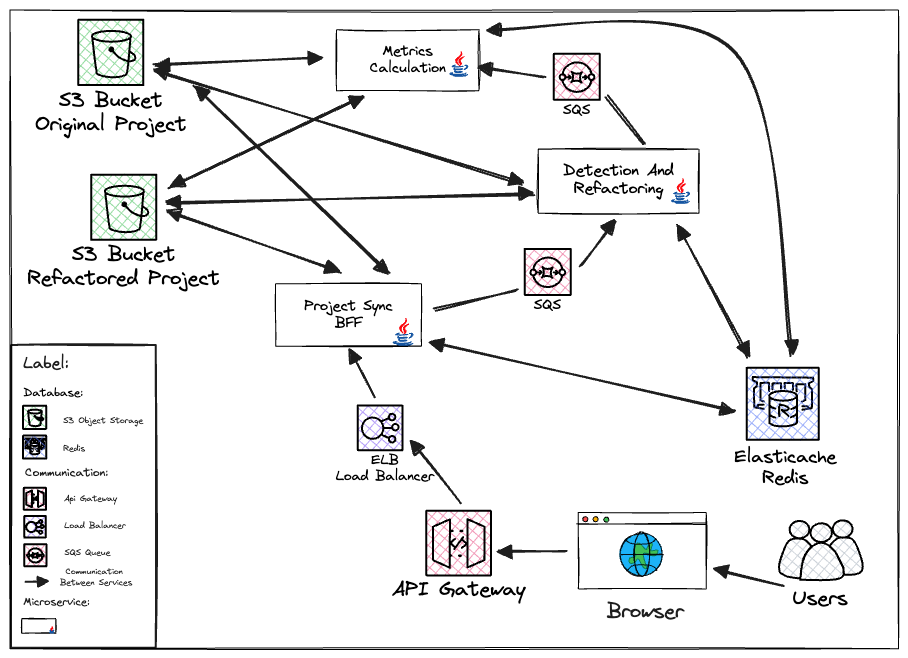
\includegraphics[width =\textwidth, scale=0.2]{Chapter-5/Figures/Async.png}
\SourceOrNote{Own authorship (2024)}
\end{figure}
\FloatBarrier

\subsection{Comunication Improvements}
\label{sub-comunication}

The communication type was switched to queues instead of HTTP requests. The modification primarily aims to establish a communication mechanism with enhanced configurability in the event of failures, as the services must acknowledge the messages, or they will be retried as often as configured. Queues also offer an asynchronous communication that is out of the box. Otherwise, in the HTTP request, the retry has to be implemented on the client side according to the server response. It is also possible to have an HTTP asynchronous request, but it must be implemented on the client side.

The Simple Queue Service (SQS) operates in its default configuration, implementing a quintuple retry mechanism to transmit a JSON object containing the project identifier between microservices.

\subsection{Storage \& Database Improvements}
\label{sub-storage}

The initial version of RMT utilizes MongoDB GridFs for file storage, a feature designed to facilitate the preservation of files within the database architecture. The updated version uses Amazon S3 for project storage, using a dual-bucket strategy: one designated for the original project and the other for the refactored iterations. All microservices are granted access to the designated buckets, enabling seamless file storage and retrieval. The project information and statuses are stored in the Redis in-memory document database, and all services have access.

\section{RMT 2.0 Packages}
\label{sec-packages}

After the architectural improvements, the package structure was reorganized and simplified. The advanced capabilities of the Spring framework, with optimizing the codebase and ensuring linear communication between services, facilitated the reduction in both the number and the size of packages.

The Project Sync BFF went through a consolidation, reducing its packages from seven to five, with none of the original packages retained. The \texttt{controller} package exposes the endpoint and initiates communication with the \texttt{refactor} package. The \texttt{refactor} package contains the entire service logic; it accesses the \texttt{ repository} package for database interactions and the \texttt{gateway} package to send messages to the subsequent service. The \texttt{configuration} package can dynamically retrieve the queue's name. Its behavior is demonstrated by the diagram on \cref{fig-project-sync-package}.

\begin{figure}[ht!]
\SetCaptionWidth{\textwidth}
\caption{Project Sync BFF package diagram}
\label{fig-project-sync-package}
\fontsize{8}{10}\selectfont
\includesvg[width =\textwidth]{Chapter-5/Figures/project-sync-bff.svg}
\SourceOrNote{Own authorship (2024)}
\end{figure}
\FloatBarrier

Progressing to the Detection and Refactoring service, a reduction in the number of packages from fourteen to seven was accomplished. The service initiates the processing via the \texttt{consumer} package, which consumes messages from a queue and retrieves a project from the database using the \texttt{repository} package as it has the database communication interface. The logic for executing refactorings is located within the \texttt{refactor} package, implementing the refactoring methods in the \texttt{methods} package, and data extraction strategies located in the \texttt{dataExtraction} package. The \texttt{gateway} package has the functionality to send messages to the queue and imports the \texttt{configuration} package to dynamically retrieve the queue name. As illustrated in \cref{fig-detection-refactoring-package}, the diagram employs two colors: yellow to signify the new packages and white to indicate the packages retained from the previous version.

\begin{figure}[ht!]
\SetCaptionWidth{\textwidth}
\caption{Detection and Refactoring service package diagram}
\label{fig-detection-refactoring-package}
\includesvg[width =\textwidth]{Chapter-5/Figures/detection-and-refactoring.svg}
\SourceOrNote{Own authorship (2024)}
\end{figure}
\FloatBarrier

The Metrics Calculator has undergone a reduction from thirteen to six packages. Consistent with the behavior of the previous service, the process starts with the \texttt{consumer} package, which retrieves messages from the queue and communicates with the database via the interface provided by the \texttt{repository} package. The retrieved database results are then used to compute quality attributes within the packages \texttt{quallityAtrributes} and \texttt{calculator}, which rely on metrics generated by the \texttt{metris} packages. The \texttt{configuration} package is responsible for instantiating the CK library \textcite{ck} for the Spring framework, allowing its injection as a dependency. The corresponding diagram is illustrated in \Cref{fig-metrics-calculator-package}, highlighting the new packages in yellow and those retained from the initial version in white.

\begin{figure}[ht!]
\SetCaptionWidth{\textwidth}
\caption{Metrics Calculator service package diagram}
\label{fig-metrics-calculator-package}
\includesvg[width =\textwidth]{Chapter-5/Figures/metrics-calculator.svg}
\SourceOrNote{Own authorship (2024)}
\end{figure}
\FloatBarrier



\section{Services Behavior Improviments}
\label{sec-services-behaivour}

Notwithstanding recent updates to the tool, its resultant behavior remains unchanged. The tool now runs with a linear execution flow, obviating the need for interservice communication during project refactoring. Given the process's asynchronous nature, users must request the completion status to display the retrieved relevant information. The process is represented in \Cref{fig-activity-diagram}, with the blue nodes representing the behavior inherited from the initial version of the tool.

\begin{figure}[ht!]
\SetCaptionWidth{\textwidth}
\caption{RMT 2.0 Activity Diagram}
\label{fig-activity-diagram}
\fontsize{5.8}{8}\selectfont
\includesvg[width =\textwidth]{Chapter-5/Figures/activity-refactored-rmt.svg}
\SourceOrNote{Own authorship (2024)}
\end{figure}
\FloatBarrier

The flow starts with the user selecting the project and sending it to the API Gateway connected to the Project Sync BFF; the service sends the project ID to the refactoring queue to start the process. The Detection and Refacred Service will immediately search for the candidates to be refactored and apply the refactoring. A message with the project ID is sent to the metrics calculation queue if any candidate is found. The Metrics Calculation Service computes the quality attributes for the project and ends the processing. The Project Sync BFF service offers a pull mechanism that consults Redis looking for a final status and, if found, returns the project information and metrics. The behavior is displayed in \Cref{fig-activity-diagram}.

\section{Testing RMT 2.0}
\label{sec-tests-2.0}

During the initial testing phase, the tool failed to refactor all files within the project. The issue was traced to the \texttt{getIfStatements} method within the AstHandle class. This method erroneously returned a single if statement rather than a comprehensive list of if statements, resulting in the refactoring being applied exclusively to the first if statement in the \cite{liu2014automated} method. Upon fixing the method, subsequent validation tests confirmed the tool's functionality as expected.

In addition to architectural improvements and code refactoring, the RMT has undergone an interface transformation by migrating from a Java-based desktop application to a browser-based one. The interface now features a selection box for project updates and two buttons, 'Evaluation' for project assessment and 'Refactor' for project refactoring. These buttons remain initially disabled, pending project selection, as depicted in \Cref{fig-factory-start}.

\begin{figure}[ht!]
\SetCaptionWidth{\textwidth}
\caption{Project Selection Page}
\label{fig-factory-start}
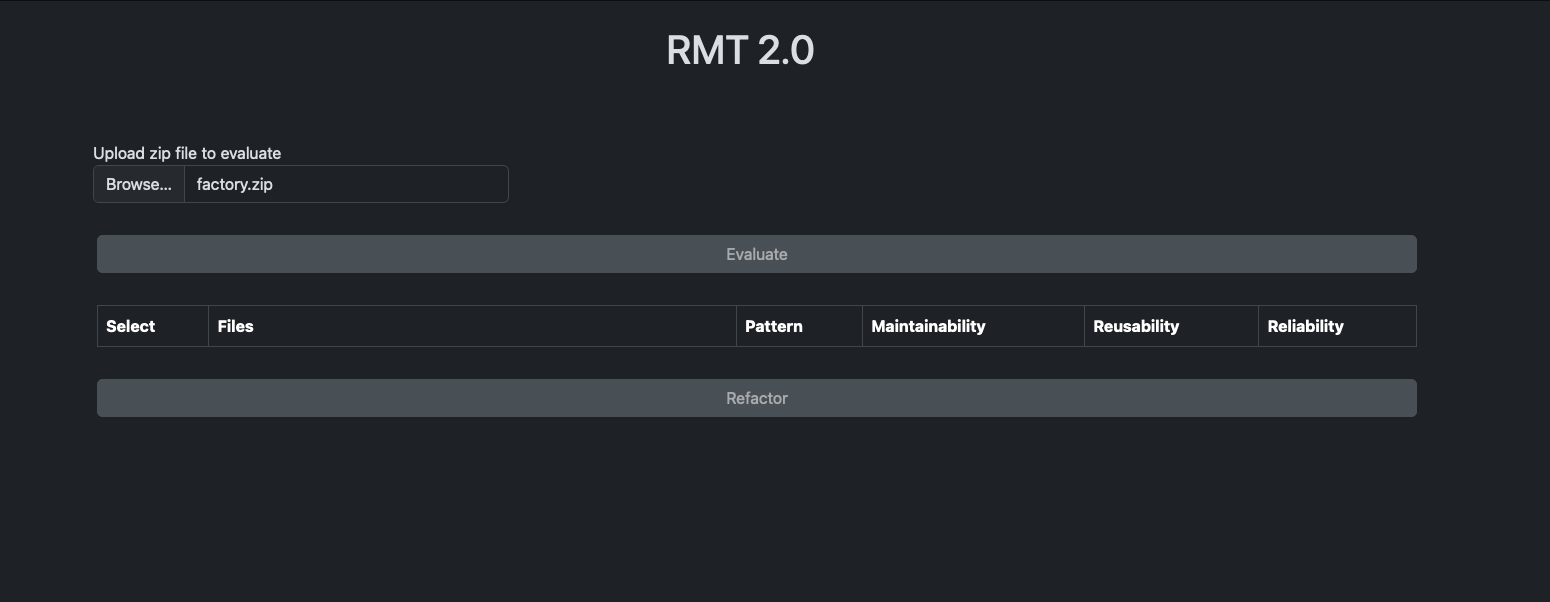
\includegraphics[width =\textwidth]{Chapter-5/Figures/rmt-factory-client-start.png}
\SourceOrNote{Own authorship (2024)}
\end{figure}
\FloatBarrier

Upon selecting the project, the 'Evaluate' button becomes active, indicated by a blue background, signifying that the project has been uploaded and the RMT backend is currently analyzing the project. This behavior is illustrated in \Cref{fig-factory-selected}.

\begin{figure}[ht!]
\SetCaptionWidth{\textwidth}
\caption{Evaluation Page}
\label{fig-factory-selected}
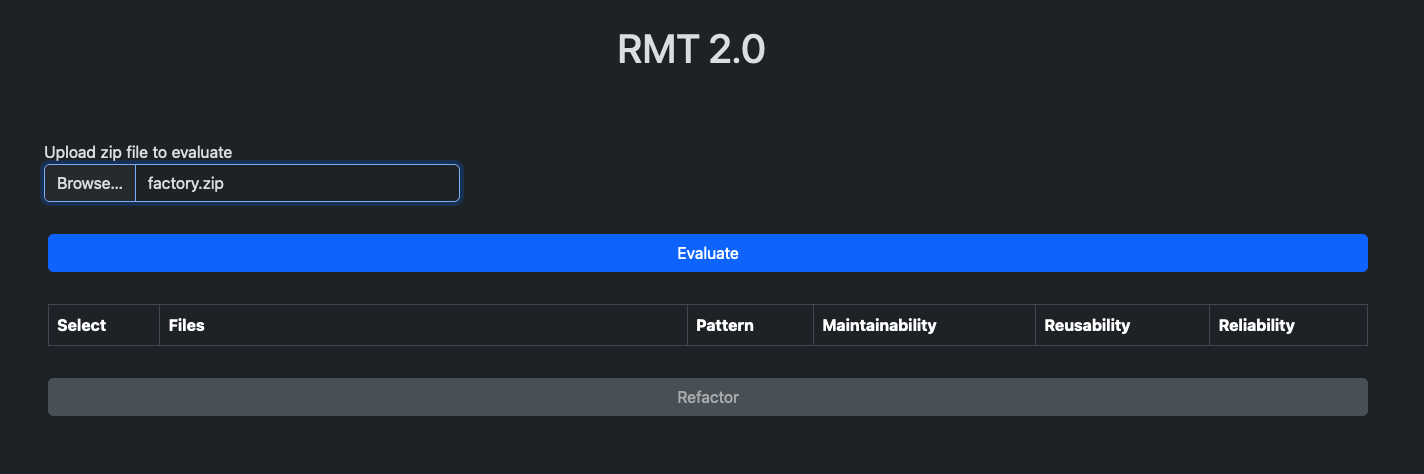
\includegraphics[width =\textwidth]{Chapter-5/Figures/rmt-factory-client-selected.png}
\SourceOrNote{Own authorship (2024)}
\end{figure}
\FloatBarrier

The refactoring candidates are shown by clicking the 'Evaluate' button. They are displayed on the table containing the refactoring information, such as the files involved, the design pattern that will be applied, and the metrics. As illustrated in \Cref{fig-factory-evaluated}.

\begin{figure}[ht!]
\SetCaptionWidth{\textwidth}
\caption{Evaluation Page}
\label{fig-factory-evaluated}
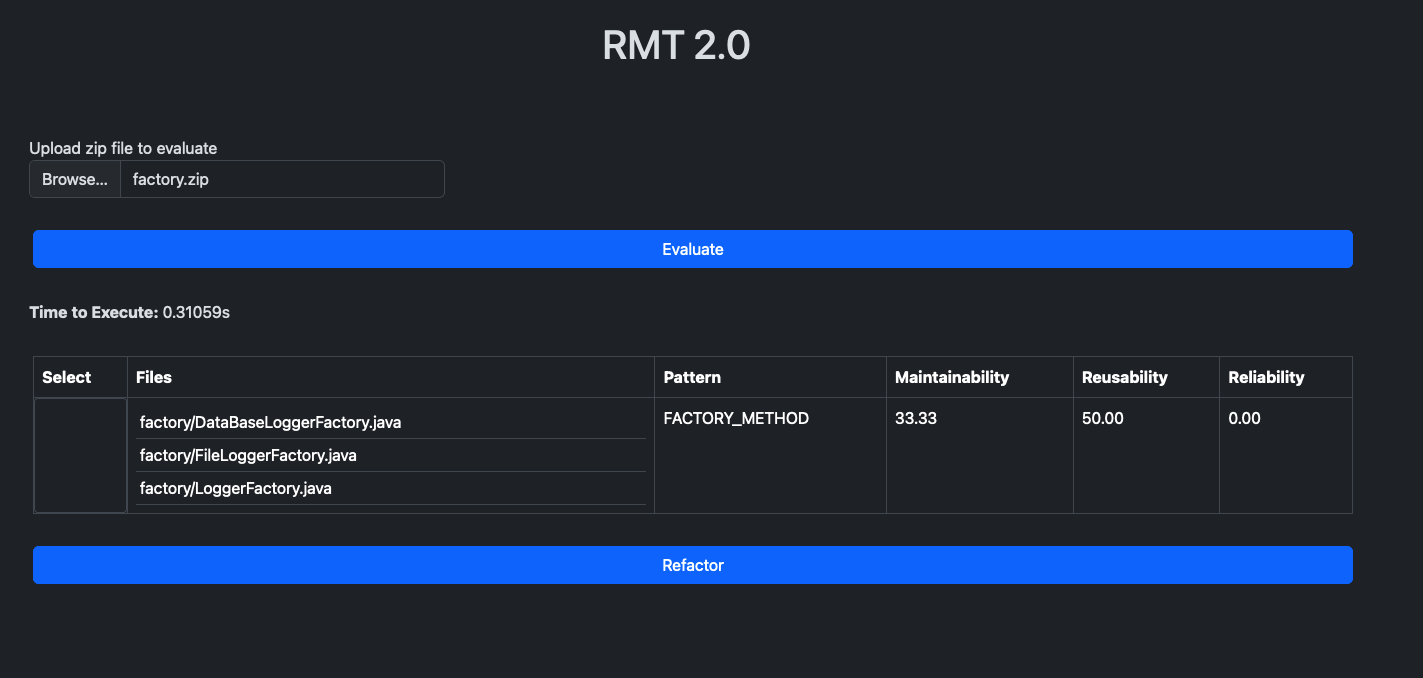
\includegraphics[width =\textwidth]{Chapter-5/Figures/rmt-factory-evaluated.png}
\SourceOrNote{Own authorship (2024)}
\end{figure}
\FloatBarrier

The refactored project can be downloaded using a link displayed after selecting a refactoring candidate in the table and clicking the 'Refactor' button. The elapsed time is shown below the 'Evaluate' button as information to the user. This is illustrated in \Cref{fig-factory-client}.

\begin{figure}[ht!]
\SetCaptionWidth{\textwidth}
\caption{Refactored Project For Factory Method Page}
\label{fig-factory-client}
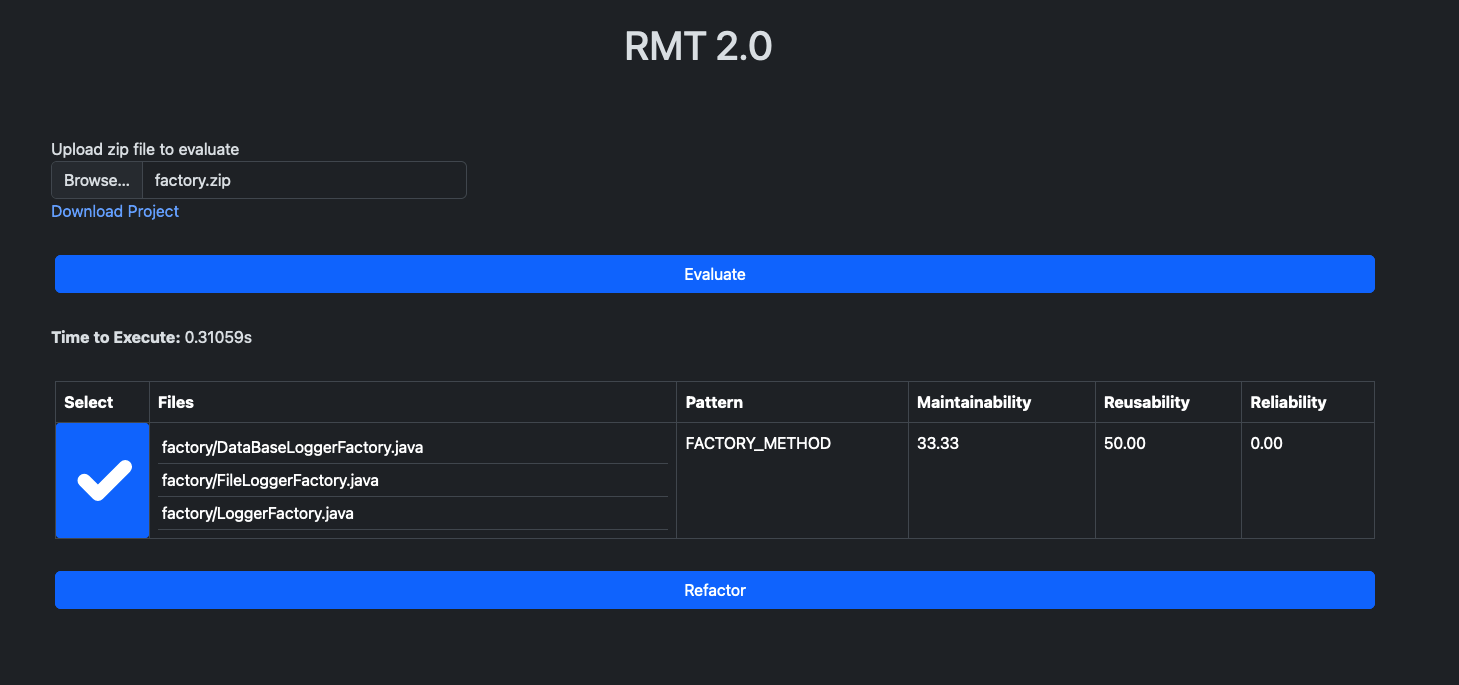
\includegraphics[width =\textwidth]{Chapter-5/Figures/rmt-factory-refactored.png}
\SourceOrNote{Own authorship (2024)}
\end{figure}
\FloatBarrier


\textcolor{red}{Pedro aqui devemos color um texto e uma image explicando o que acontece quando a pessoa aceite realizar a refatoração. Assim, fica claro o processo. O que acha?}


\subsection{Testing Through Refactored Article Application Exemplars}
\label{sub-testing-article}

The implementations exemplified by \textcite{liu2014automated} and \textcite{zafeiris2017automated} were used for the preliminary evaluation.

To refactor using the factory method design pattern, \textcite{liu2014automated} introduces four distinct classes: a \texttt{Logger} interface, 	\texttt{FileLogger} and \texttt{DatabaseLogger} which implement the interface, and the \texttt{LoggerFactory} serving as a factory to select among the implementations. The \Cref{fig-factory-client} displays the refactored \texttt{LoggerFactory} that was changed to abstract; the implementation was moved to the \texttt{FileLoggerFactory} and \texttt{DatabaseLoggerFactory}. The metrics displayed are positive, indicating an improvement in maintainability and reusability without changing reliability.

To exemplify the strategy pattern \textcite{liu2014automated}, create the \texttt{MovieTicket} class, which has an if statement for each ticket type. The method creates an abstract \texttt{Strategy} class with the calculate method, the code extracted from the \texttt{MovieTicket} is implemented on the \texttt{ConcreteStrategyS}, \texttt{ConcreateStrategyM} and \texttt{ConcreateStrategyC}. The maintenance and reusability metrics improved, although reliability decreased, as shown in \Cref{fig-strategy-client}.

\begin{figure}[ht!]
\caption{Refactored Project For Strategy}
\label{fig-strategy-client}
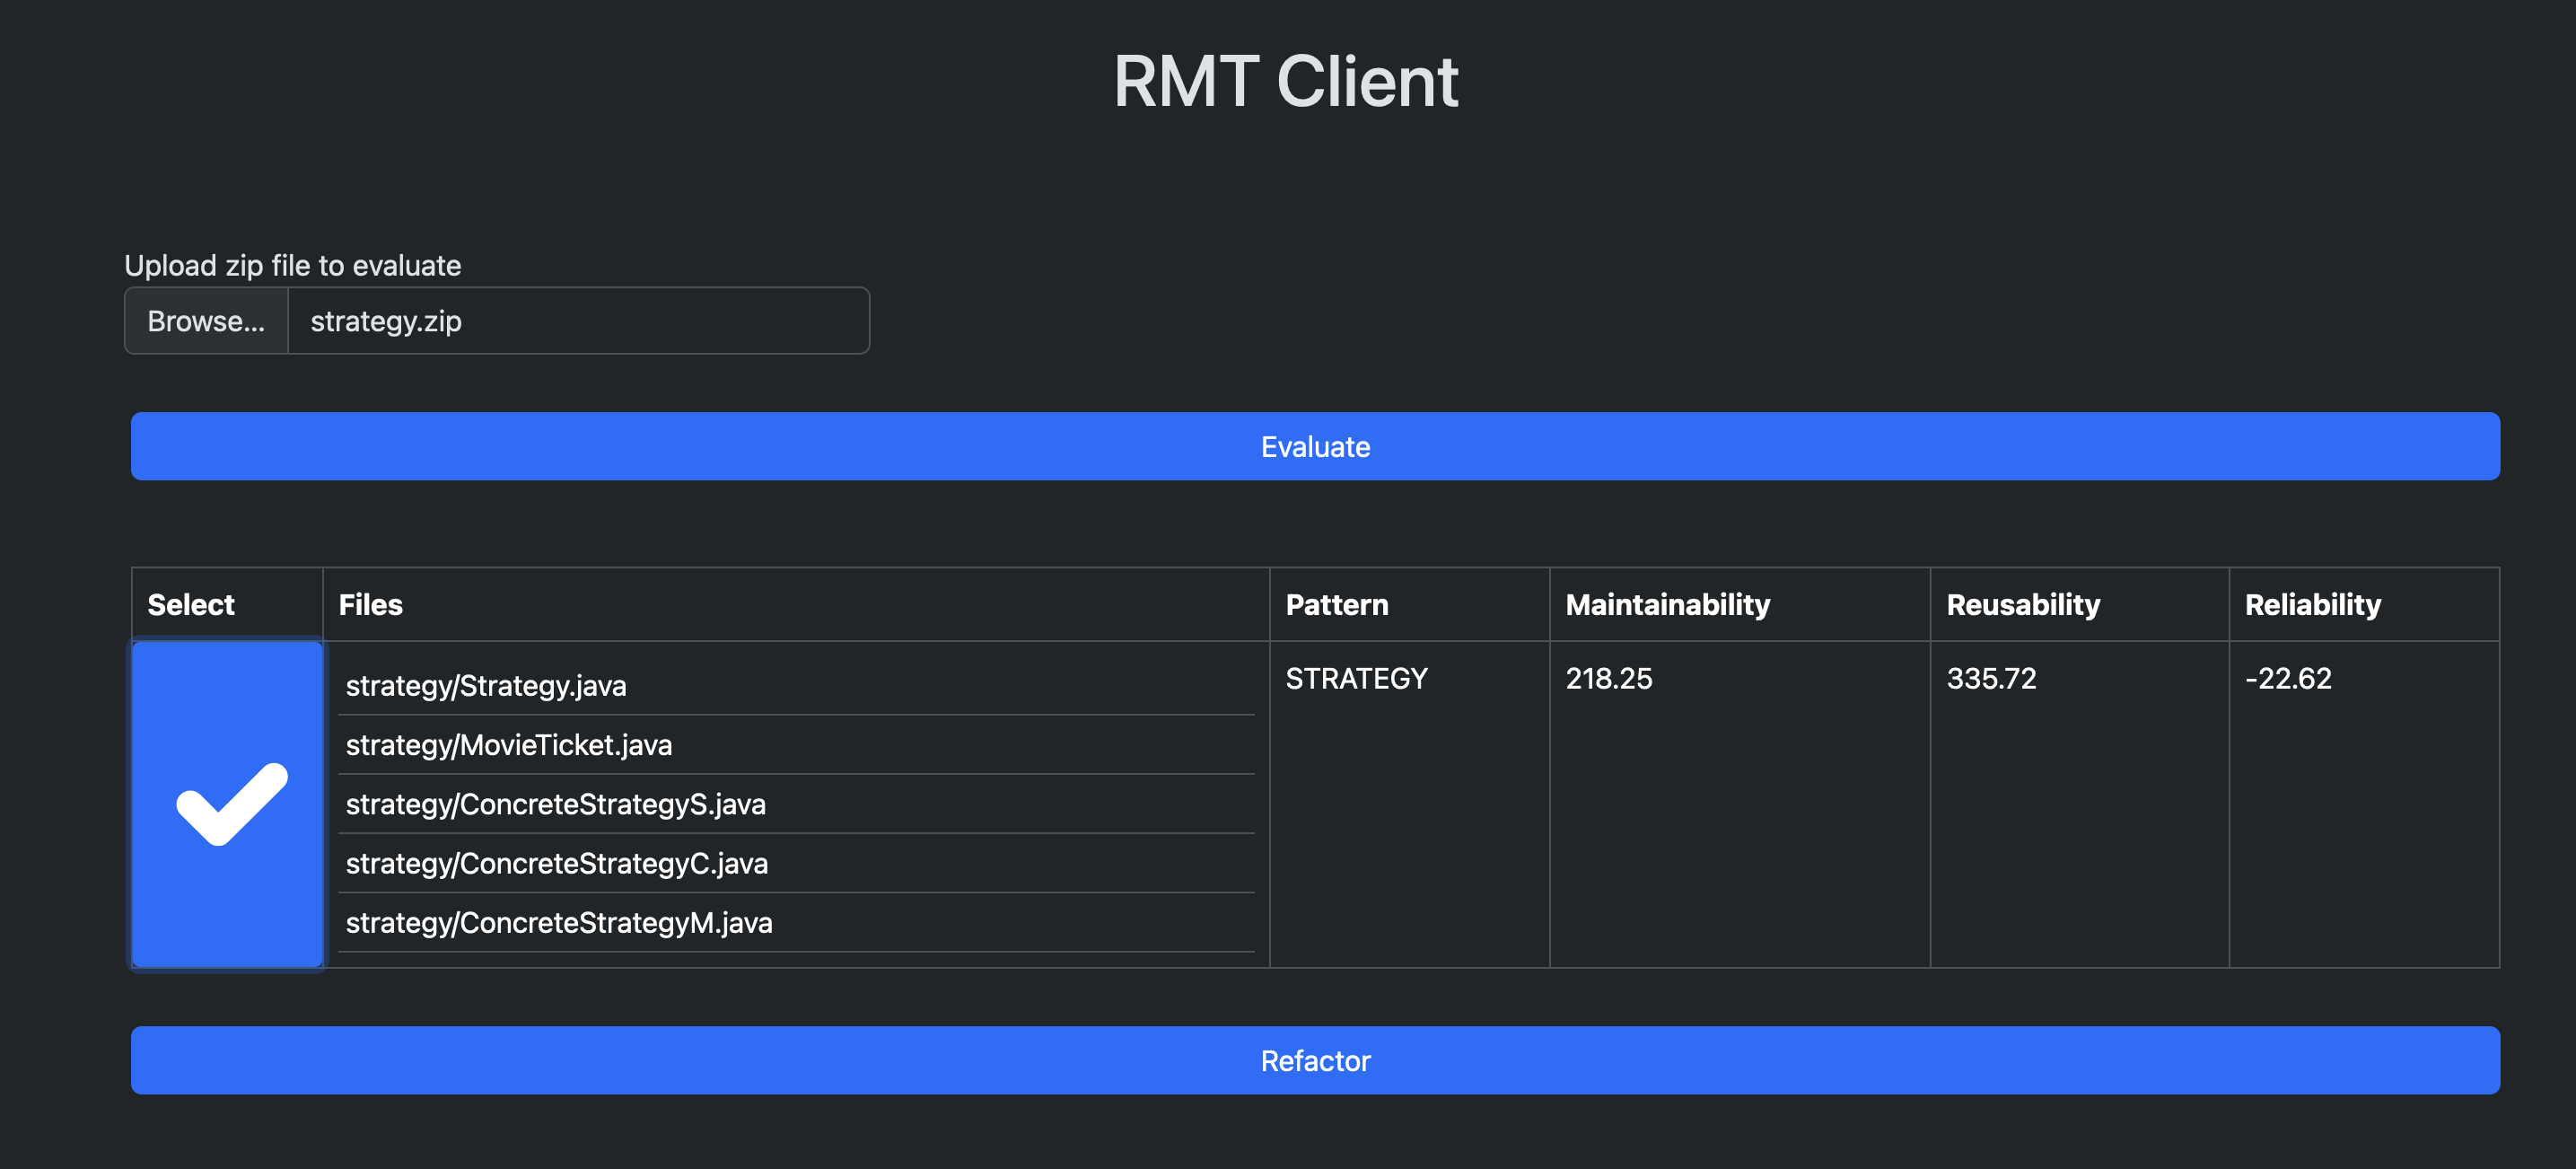
\includegraphics[width =\textwidth]{Chapter-5/Figures/rmt-strategy-client.png}
\SourceOrNote{Own authorship (2024)}
\end{figure}
\FloatBarrier

The \textcite{zafeiris2017automated} implements the template method using the jade-test-suit to exemplify the process. The \texttt{JICPPeer} class is the parent of the \texttt{JICPSPeer} class, which implements a method that has a \texttt{super} call; the refactoring extract code before and after the super call into new methods and replaces the super call to a method call with the same behavior. The maintainability, reusability, and reliability metrics are negative, showing a deterioration. It is represented in \Cref{fig-template-client}

\begin{figure}[ht!]
\caption{Refactored Project For Template Method}
\label{fig-template-client}
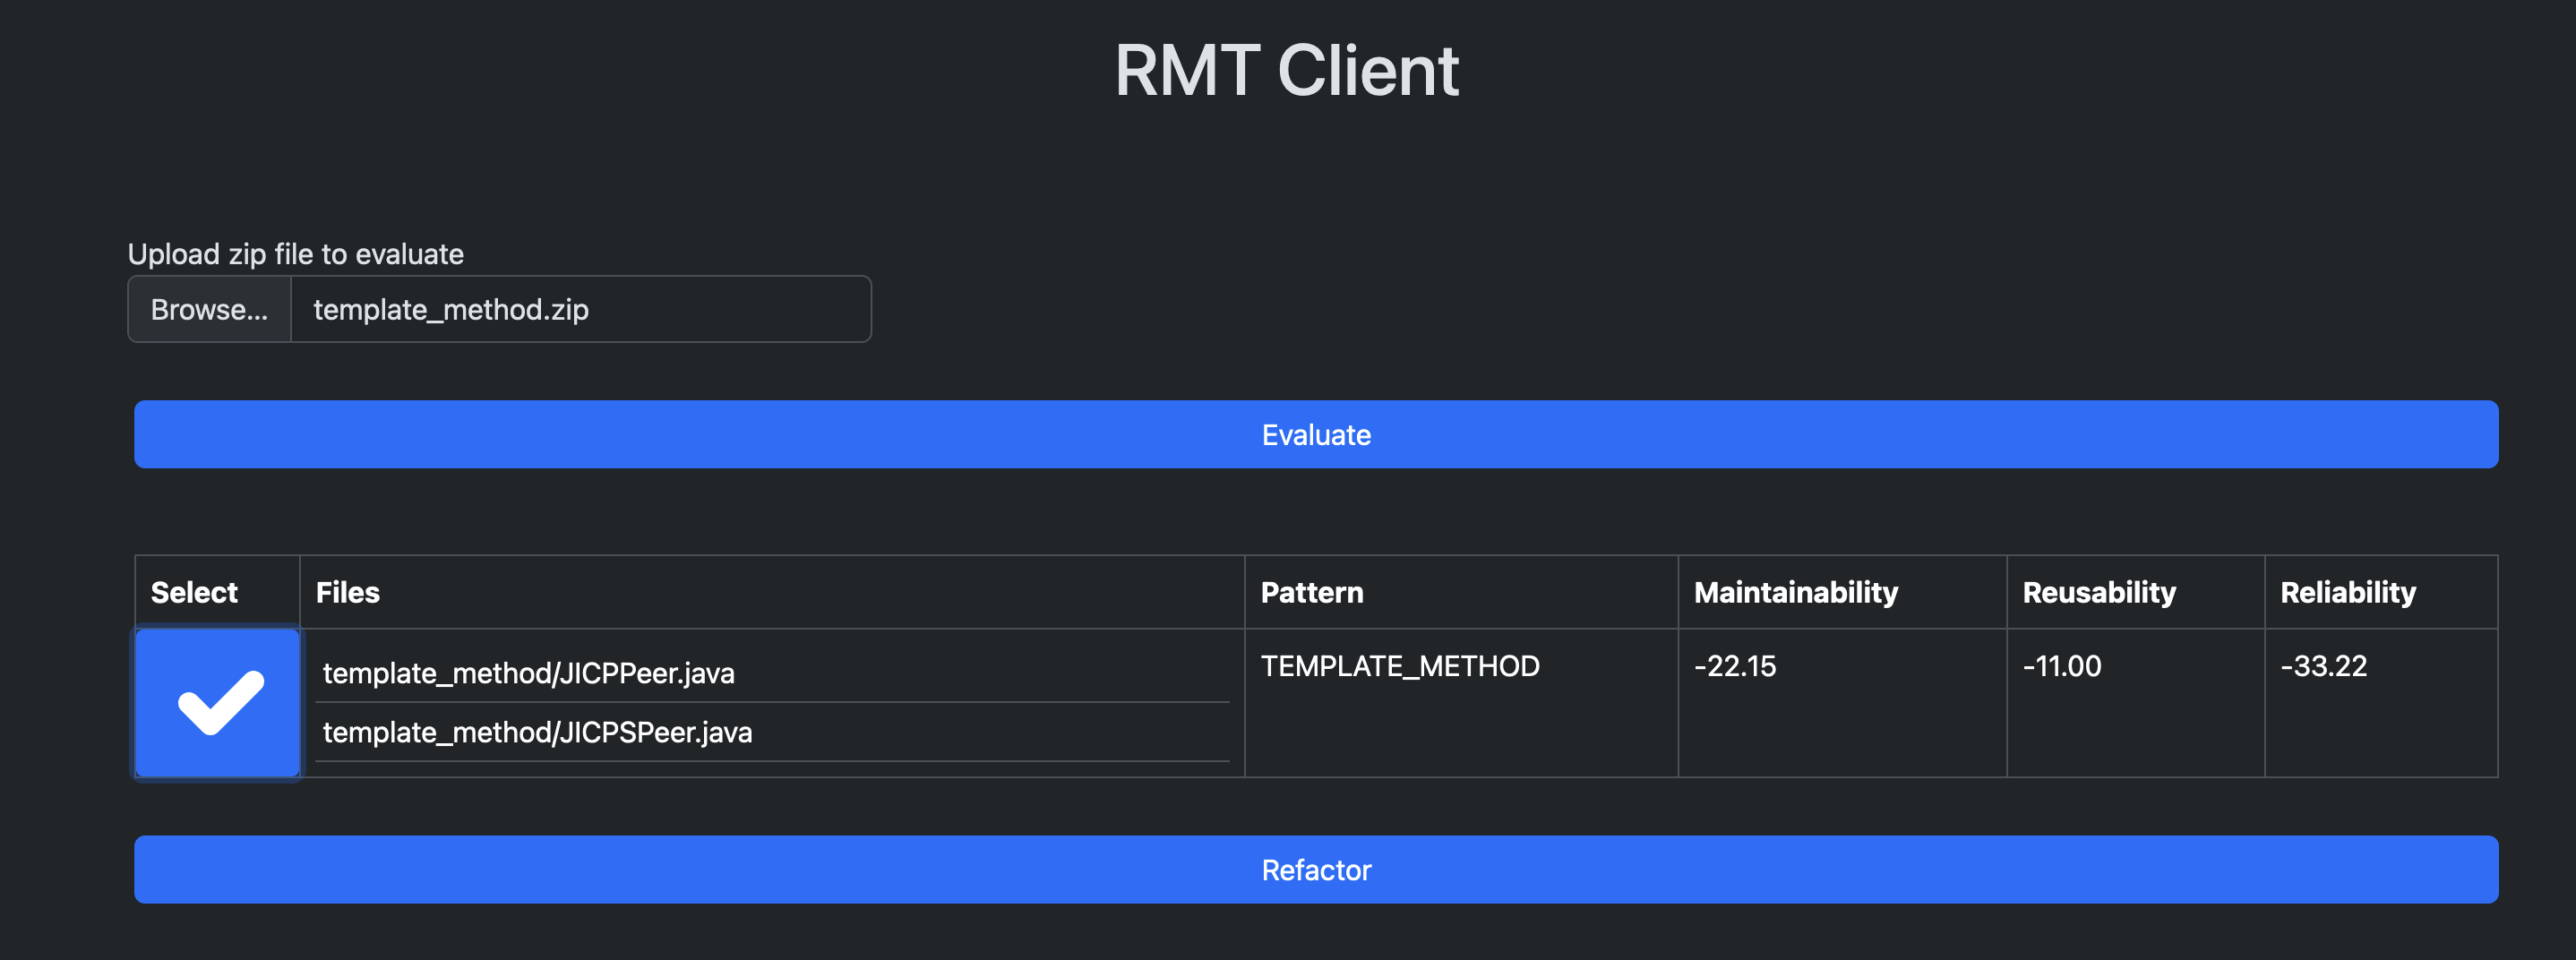
\includegraphics[width =\textwidth]{Chapter-5/Figures/rmt-template-client.png}
\SourceOrNote{Own authorship (2024)}
\end{figure}
\FloatBarrier

An additional approach to test the tool and ensure its quality will undergo a self-scanning procedure. The analysis was performed to test the effectiveness of the tool, with a focus on evaluating RMT and its next version, RMT 2.0. Examining both RMT versions showed that there were no elements that needed refactoring. 

\subsection{Testing With Real Projects}
\label{sub-testing-real}

The new version of the tool has been tested against real-world projects to ensure that it maintains the initial functionality. To evaluate the RMT, \textcite{beluzzo2018abordagem}, select fifty projects from Github; from those projects, the RMT found candidate refactoring in seventeen projects. All these projects are shown on \cref{tab-projects-classes}; most of the projects have been updated after \cite{beluzzo2018abordagem} testing.

\begin{table}[!htbp]
  \centering
  \caption{List of Projects For Test Cases}
  \begin{tabular}{e{},{}@{}lc}
    \toprule
    \textbf{\#} & \textbf{Projects} & \textbf{Nº of classes} \\
    \midrule
    p1  & \href{https://github.com/evant/gradle-retrolambda.git}{https://github.com/evant/gradle-retrolambda.git}                               & 23  \\
    p2  & \href{https://github.com/Progether/JAdventure.git}{https://github.com/Progether/JAdventure.git}                                       & 64  \\
    p3  & \href{https://github.com/menacher/java-game-server.git}{https://github.com/menacher/java-game-server.git}                             & 187 \\
    p4  & \href{https://github.com/google/caliper.git}{https://github.com/google/caliper.git}                                                   & 269 \\
    p5  & \href{https://github.com/Devskiller/jfairy.git}{https://github.com/Devskiller/jfairy.git}                                             & 90  \\
    p6  & \href{https://github.com/jpush/jpush-api-java-client.git}{https://github.com/jpush/jpush-api-java-client.git}                         & 120 \\
    p7  & \href{https://github.com/dain/leveldb.git}{https://github.com/dain/leveldb.git}                                                       & 106 \\
    p8  & \href{https://github.com/census-instrumentation/opencensus-java.git}{https://github.com/census-instrumentation/opencensus-java.git}   & 626 \\
    p9  & \href{https://github.com/raml-org/raml-java-parser}{https://github.com/raml-org/raml-java-parser}                                     & 458 \\
    p10 & \href{https://github.com/Javacord/Javacord.git}{https://github.com/Javacord/Javacord.git}                                             & 1100 \\
    p11 & \href{https://github.com/maxmind/geoip-api-java.git}{https://github.com/maxmind/geoip-api-java.git}                                   & 28  \\
    p12 & \href{https://github.com/kwhat/jnativehook.git}{https://github.com/kwhat/jnativehook.git}                                             & 56  \\
    p13 & \href{https://github.com/cardillo/joinery.git}{https://github.com/cardillo/joinery.git}                                               & 51  \\
    p14 & \href{https://github.com/Kurento/kurento-java.git}{https://github.com/Kurento/kurento-java.git}                                       & 600 \\
    p15 & \href{https://github.com/joscha/play-authenticate.git}{https://github.com/joscha/play-authenticate.git}                               & 126 \\
    p16 & \href{https://github.com/caprica/vlcj.git}{https://github.com/caprica/vlcj.git}                                                       & 364 \\
    p17 & \href{https://github.com/careermonk/DataStructureAndAlgorithmsMadeEasyInJava.git}{https://github.com/careermonk/DataStructureAndAlgorithmsMadeEasyInJava.git} & 148 \\
    \bottomrule
  \end{tabular}
    \SourceOrNote{Own authorship (2024)}
  \label{tab-projects-classes}
\end{table}
\FloatBarrier

The tool was tested using the same updated projects. The \cref{tab-software-project-metrics} shows the results for the refactoring, with all the classes that could be refactored. The table displays the pattern by referring to the template method of T, the strategy by S, and the resulting metrics in percentage for each refactoring candidate.

Following an analysis of the empirical results, it is immediately evident that the application of the factory method was not identified in any of the examined projects. The distribution of candidates for the template method and the strategy pattern is balanced, with 14 classes favoring the strategy pattern characterizing 43.8\% of candidates and 18 classes corresponding to the template method equivalent to 56. 2\% of classes. Project two is not on the table as it had no candidates for refactoring.

Testing project two on RMT 1.0 shows a possible refactoring, but by debuting the tool and analyzing the post-refactoring files, was likely to find the same issue described in \cref{subsub-limitation}, where an Ast handler method has a bug that only returns one if statement from the method, making it accept the refactoring without evaluating the other ifs on the method.

Regarding the strategy method, specific projects may have two candidates for a single class. This occurrence is attributable to the candidate identification process, in which a class encompasses two methods for refactoring. Analyzing the metrics, most projects demonstrated improved maintainability and reusability, accompanied by decreased reliability. These findings suggest that strategy-based refactoring predominantly benefits developers based on the utilized metrics.

Nevertheless, the template method has shown reductions in all metrics, with deviations that do not exceed a threshold of 1\%. The displayed metrics enable developers to make knowledgeable decisions about project refactoring; despite minor degradations in these metrics, a developer might still opt to refactor the class.

\textcolor{red}{acho que aqui poderia apresentar um gráfico comparando os projetos por tipo de atributo. Por exemplo, um gráfico apresentado a manutenibilidade, etc... O que acha?}

\begin{longtable}{ccp{5.1cm}ccc@{}}
%% Cabeçalho da primeira página
\caption{Refactored Projects Metrics and Classes}
\label{tab-software-project-metrics}                          \\[\belowcaptionskip]
\multicolumn{6}{@{}r@{}}{\textbf{(continue)}}                 \\[\belowcaptionskip]
\toprule%
\multicolumn{1}{@{}c}{\textbf{Project}}            &
\multicolumn{1}{c}{\textbf{Pattern}}               &
\multicolumn{1}{c}{\textbf{Class}}                 &
\multicolumn{1}{c}{\textbf{Maintainability}}       &
\multicolumn{1}{c}{\textbf{Reusability}}           &
\multicolumn{1}{c@{}}{\textbf{Reliability}}        \\
\midrule%
\endfirsthead%
%% Cabeçalho das páginas (exceto primeira e última)
\caption[]{Refactored Projects Metrics and Classes}           \\[\belowcaptionskip]
\multicolumn{6}{@{}r@{}}{\textbf{(continuation)}}             \\[\belowcaptionskip]
\toprule%
\multicolumn{1}{@{}c}{\textbf{Project}}            &
\multicolumn{1}{c}{\textbf{Pattern}}               &
\multicolumn{1}{c}{\textbf{Class}}                 &
\multicolumn{1}{c}{\textbf{Maintainability}}       &
\multicolumn{1}{c}{\textbf{Reusability}}           &
\multicolumn{1}{c@{}}{\textbf{Reliability}}        \\
\midrule%
\endhead%
%% Cabeçalho da última página
\caption[]{Refactored Projects Metrics and Classes}           \\[\belowcaptionskip]
\multicolumn{6}{@{}r@{}}{\textbf{(conclusion)}}               \\[\belowcaptionskip]
\toprule%
\multicolumn{1}{@{}c}{\textbf{Project}}            &
\multicolumn{1}{c}{\textbf{Pattern}}               &
\multicolumn{1}{c}{\textbf{Class}}                 &
\multicolumn{1}{c}{\textbf{Maintainability}}       &
\multicolumn{1}{c}{\textbf{Reusability}}           &
\multicolumn{1}{c@{}}{\textbf{Reliability}}        \\
\midrule%
\endlasthead%
%% Rodapé da última página
\bottomrule%
\LTSourceOrNote{Own authorship (2024)}           \\
\endlastfoot% 
  p1 & S & Feature.java & 3.25 & 5.45 & -0.90 \\
  p1 & S & Lib.java & 3.25 & 5.45 & -0.90 \\
  p3 & S & JetlangEventDispatcher.java & 0.24 & 0.38 & -0.06 \\
  p3 & T & AbstractNettyServer.java & -0.10 & -0.06 & -0.16 \\
  p3 & T & DefaultSessionEventHandler.java & -0.13 & -0.08 & -0.20 \\
  p4 & S & ShortDuration.java & 0.15 & 0.23 & 0 \\
  p5 & S & PlVATIdentificationNumberProvider.java & 0.43 & 0.71 & -0.16 \\
  p5 & T & FairyModule.java & -0.62 & -0.25 & -0.94 \\
  p6 & T & PlatformNotification.java & -0.20 & -0.10 & -0.30 \\
  p7 & S & Slices.java & 0.44 & 0.68 & -0.06 \\
  p7 & S & Slices.java & 0.44 & 0.68 & -0.06 \\
  p8 & S & BenchmarksUtil.java & 0.10 & 0.16 & -0.02 \\
  p8 & S & BenchmarksUtil.java & 0.10 & 0.16 & -0.02 \\
  p8 & S & StackdriverExportUtils.java & 0.07 & 0.10 & -0.02 \\
  p8 & T & AbstractMvcIntegrationTest.java & -0.03 & -0.02 & -0.04 \\
  p8 & T & HttpServletFilter.java & -0.03 & -0.02 & -0.05 \\
  p9 & T & ReferenceSuggester.java & -0.05 & -0.03 & -0.08 \\
  p10 & T & SlashCommandBuilderDelegateImpl.java & -0.02 & -0.02 & -0.04 \\
  p10 & T & TextableRegularServerChannelUpdater-DelegateImpl.java & -0.03 & -0.02 & -0.04 \\
  p10 & T & ServerThreadChannelUpdater-DelegateImpl.java & -0.04 & -0.02 & -0.06 \\
  p10 & T & ServerVoiceChannelUpdater-DelegateImpl.java & -0.03 & -0.02 & -0.05 \\
  p10 & T & ServerVoiceChannelUpdater-DelegateImpl.java & -0.05 & -0.03 & -0.08 \\
  p11 & S & LookupService.java & 3.21 & 4.82 & -0.03 \\
  p12 & T & NativeMouseEvent.java & -0.31 & -0.20 & -0.46 \\
  p12 & T & NativeInputEvent.java & -0.39 & -0.25 & -0.58 \\
  p13 & S & DataFrameAdapter.java & 0.43 & 0.69 & -0.08 \\
  p14 & S & JsonRpcConnectionListenerKurento.java & 0.05 & 0.08 & -0.02 \\
  p14 & T & AbstractJsonRpcClientWebSocket.java & -0.03 & -0.02 & -0.04 \\
  p15 & T & OAuth1AuthProvider.java & -0.18 & -0.10 & -0.28 \\
  p16 & T & TrackInfo.java & -0.12 & -0.09 & -0.18 \\
  p16 & T & Track.java & -0.18 & -0.13 & -0.26 \\
  p17 & S & FibonacciWithDP.java & 0.89 & 1.37 & -0.10 \\
  \bottomrule
\end{longtable}
\FloatBarrier

\section{Comparing RMT versions}
\label{sec-comparing}

Following the evaluation of the tool, the next stage involves assessing the efficacy of the RMT's remodeling. As noted in \cref{subsub-limitation}, the initial version of the tool demonstrated issues in handling 'if' statements within the Template Method and Strategy design patterns. Consequently, it impeded a direct comparison of metrics between the tools, as the refactoring results would inherently differ, leading to variations in the calculated results.

One of the hypotheses proposed through the refactoring of the tool is that RMT 2.0 exhibits superior performance compared to version 1.0. Both tools were subjected to a comparative analysis by executing the 16 projects of \cref{tab-projects-classes} to validate this claim. The experiments were carried out on a MacBook Air M1 with 8GB of RAM; all other programs were closed, and the computer was plugged in to deliver the most power.

For the first version, the MongoDB 5.0.28 \cite{mongo} database was deployed using Docker, complemented by the WildFly 19 \cite{wildfly} server for the service deployment. Adjustments were necessary to allocate JVM memory from 512 MB to 2048 MB on the wildfly server to analyze larger projects successfully.

In the second version, the entire deployment was containerized using Docker \cite{docker}. The database service was managed using Redis \cite{Redis} version 7.2.4, while Localstack \cite{localstack} version 3.02 was used to provision the SQS queue and S3 storage. The Spring Framework \cite{spring} incorporates an embedded server, eliminating the need for an external application server such as WildFly and enabling the application deployment as a container.

The \Cref{fig-time-chart} shows the execution times for the fifteen projects. In particular, project p8 failed to run under RMT 1.0, which caused an error on every attempt. The projects with a time difference greater than 50\% were tested three times to ensure that the computer did not cause the performance error at the time; the minimum time of the three executions is represented in the table. 

\begin{table}[!htbp]
    \label{tab-comparison-rmt}
    \centering
    \caption{Comparison of RMT 1.0 and RMT 2.0 Execution Time}
    \begin{tabular}{e{},{}@{}lllcc}
        \toprule
        \textbf{Projects} & \textbf{RMT 1.0} & \textbf{RMT 2.0} & \textbf{Diff In Seconds} & \textbf{Diff In Percentage} & \textbf{Project Size} \\
        \midrule
        p1 & 1,62768s & 0,72107s & 0,90661 & 55,70\% & 23 \\
        p3 & 14,75962s & 5,14317s & 9,61645 & 65,15\% & 187 \\
        p4 & 8,01335s & 3,15658s & 4,85677 & 60,61\% & 269 \\
        p5 & 9,76558s & 1,36931s & 8,39627 & 85,98\% & 90 \\
        p6 & 14,31251s & 1,6893s & 12,62321 & 88,20\% & 120 \\
        p7 & 3,27219s & 2,81377s & 0,45842 & 14,01\% & 106 \\
        p9 & 22,59097s & 3,4106s & 19,18037 & 84,90\% & 458 \\
        p10 & 141,6649s & 24,86174s & 116,80316 & 82,45\% & 1100 \\
        p11 & 3,4375s & 1,3395s & 2,098 & 61,03\% & 28 \\
        p12 & 3,29823s & 1,29021s & 2,00802 & 60,88\% & 56 \\
        p13 & 2,26107s & 1,77315s & 0,48792 & 21,58\% & 51 \\
        p14 & 37,42521s & 7,69026s & 29,73495 & 79,45\% & 600 \\
        p15 & 7,33497s & 1,14457s & 6,1904 & 84,40\% & 126 \\
        p16 & 14,69265s & 3,81467s & 10,87798 & 74,04\% & 364 \\
        p17 & 2,09381s & 1,33635s & 0,75746 & 36,18\% & 148 \\
        \bottomrule
    \end{tabular}
    \SourceOrNote{Own authorship (2024)}
\end{table}
\FloatBarrier

Through detailed analysis of execution durations, it became apparent that the projects exhibiting extended execution times comprised more classes as in \Cref{fig-time-by-size} and were refactored for the template method. Specifically, projects p3, p5, p6, p9, p10, p12, p14, p15, and p16, which incorporated the Template Method refactoring, demonstrated a significant discrepancy in execution time when contrasting both tool versions. This discrepancy arises due to performance-focused optimizations implemented within the method code and the overall tool.

\begin{figure}[ht!]
\caption{Execution time difference between RMT version}
\label{fig-time-chart}
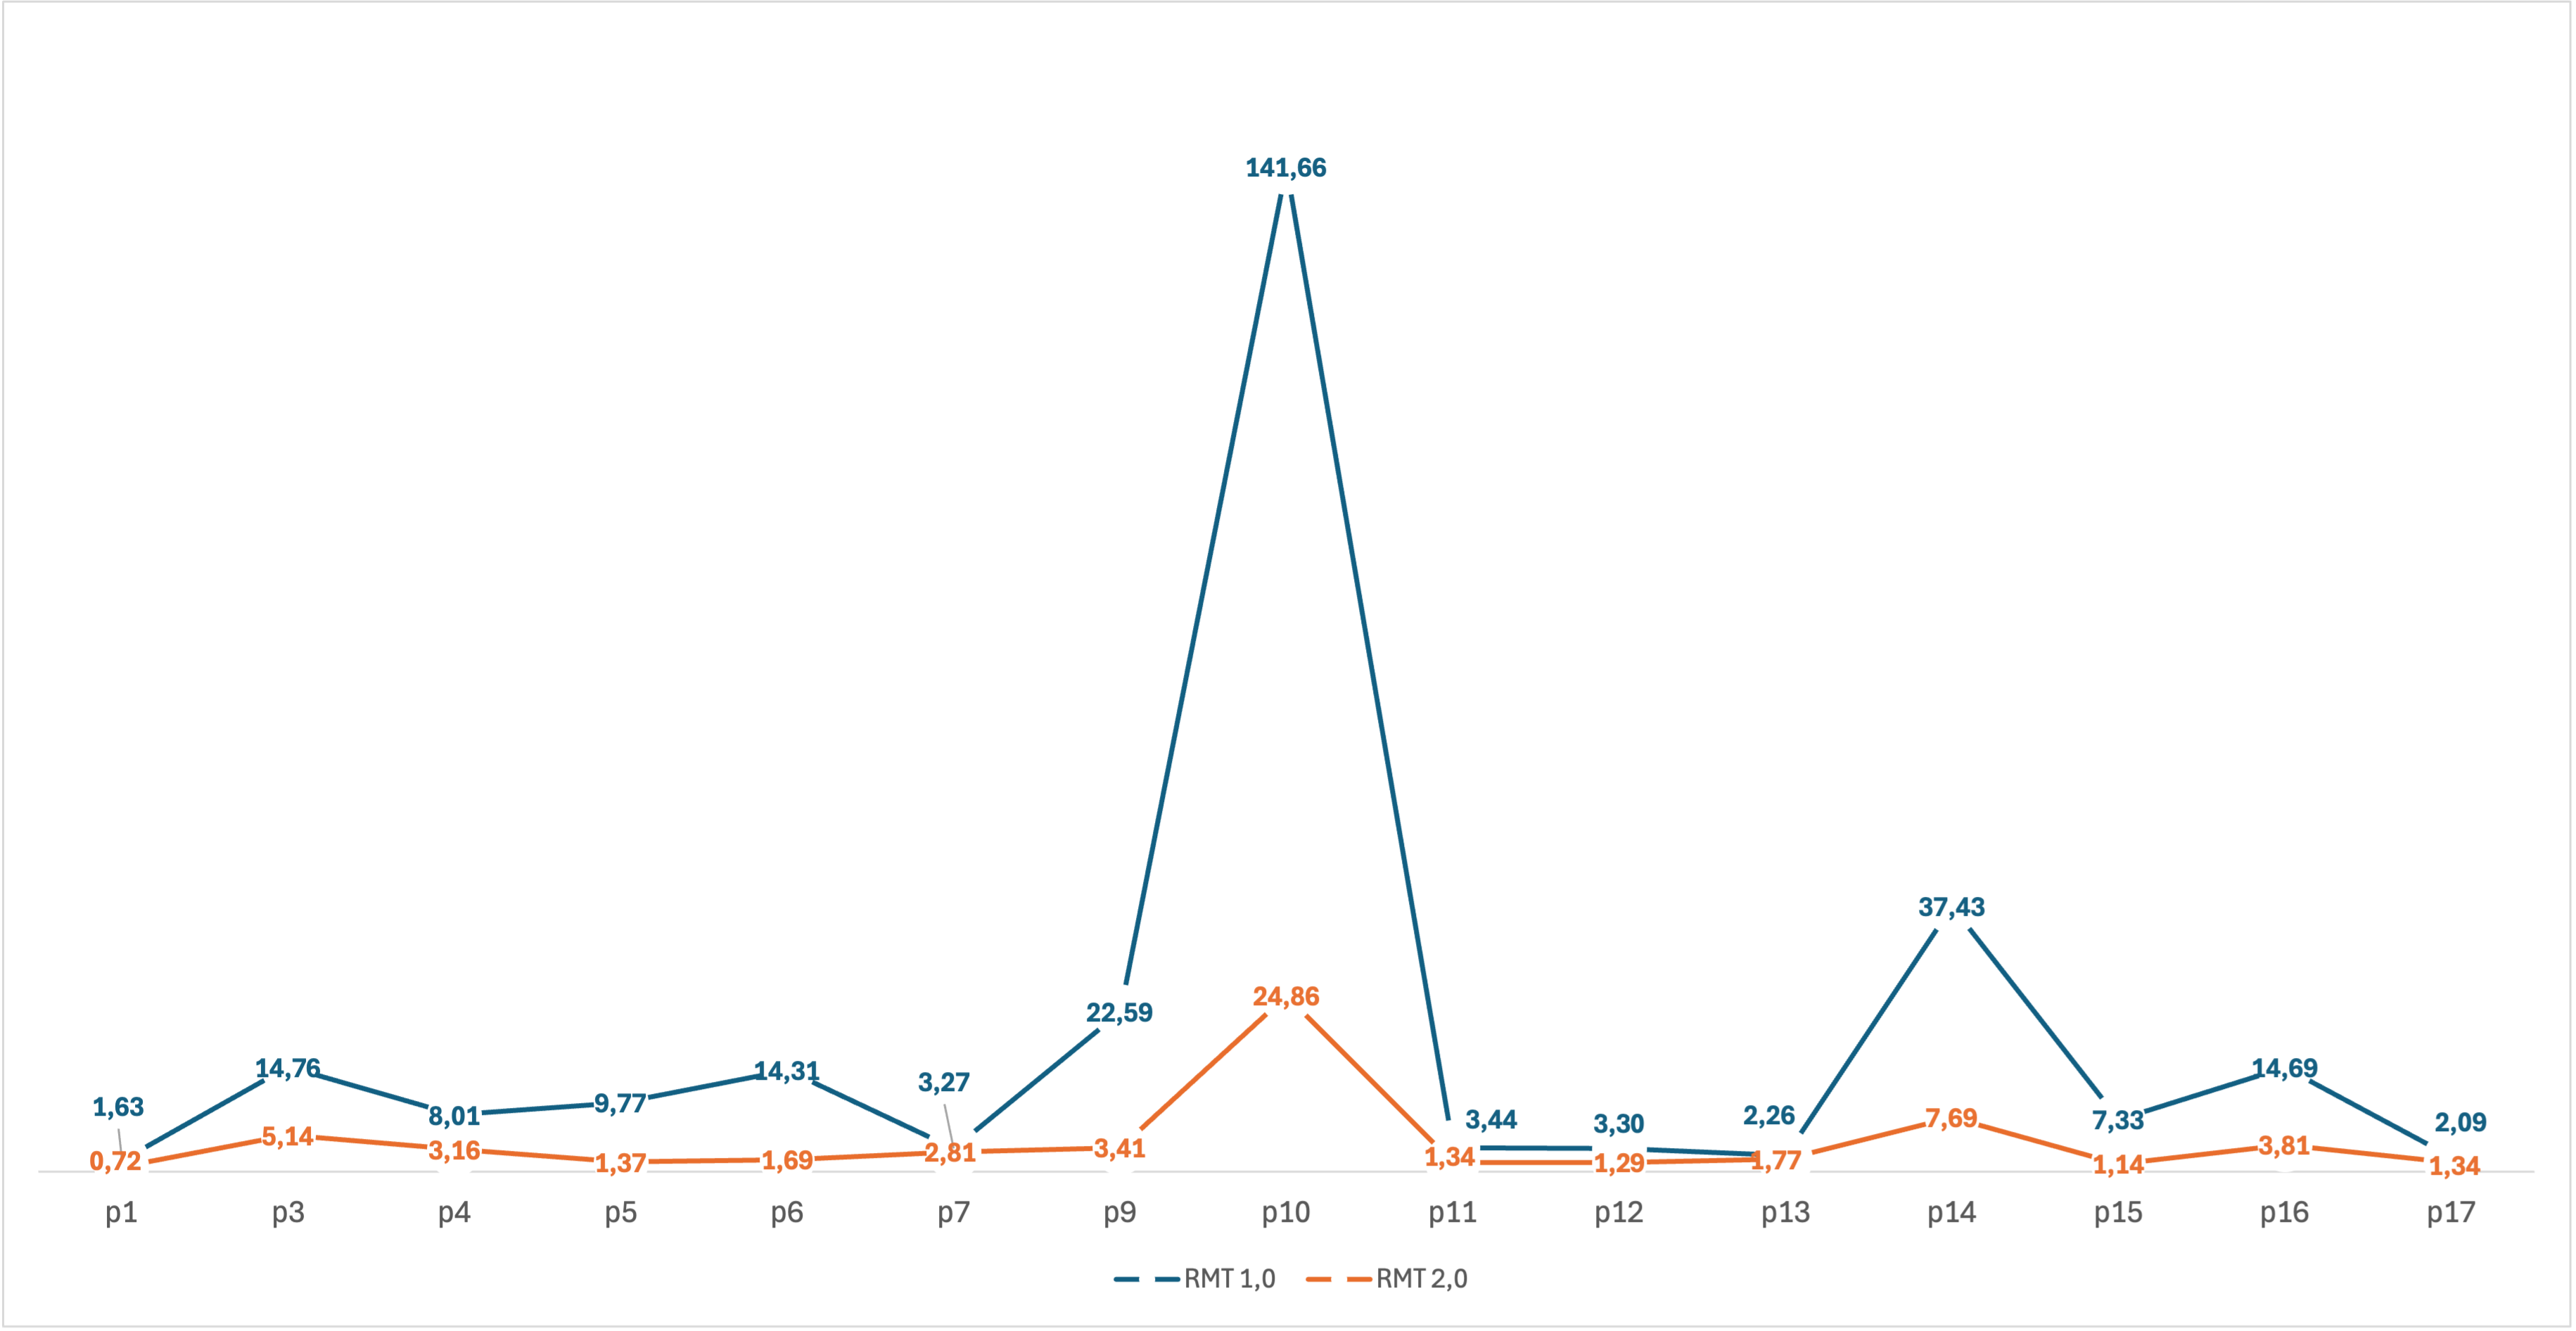
\includegraphics[width =\textwidth]{Chapter-5/Figures/time-diff.png}
\SourceOrNote{Own authorship (2024)}
\end{figure}
\FloatBarrier

The RMT 2.0 exhibited a substantial decrease in execution time by 63.64\%. This reduction was particularly found in the projects p5, p6, p9, p10, p14, p15 and p16, with over 80\% reductions recorded in projects p5, p6, p9, p10 and p15. In particular, excluding p5, all these projects have more than 100 classes. The larger difference between projects is in p9 and p10, which have 458 and 1100 classes, respectively. 

\begin{figure}[ht!]
\caption{Execution time difference by project size between RMT version}
\label{fig-time-by-size}
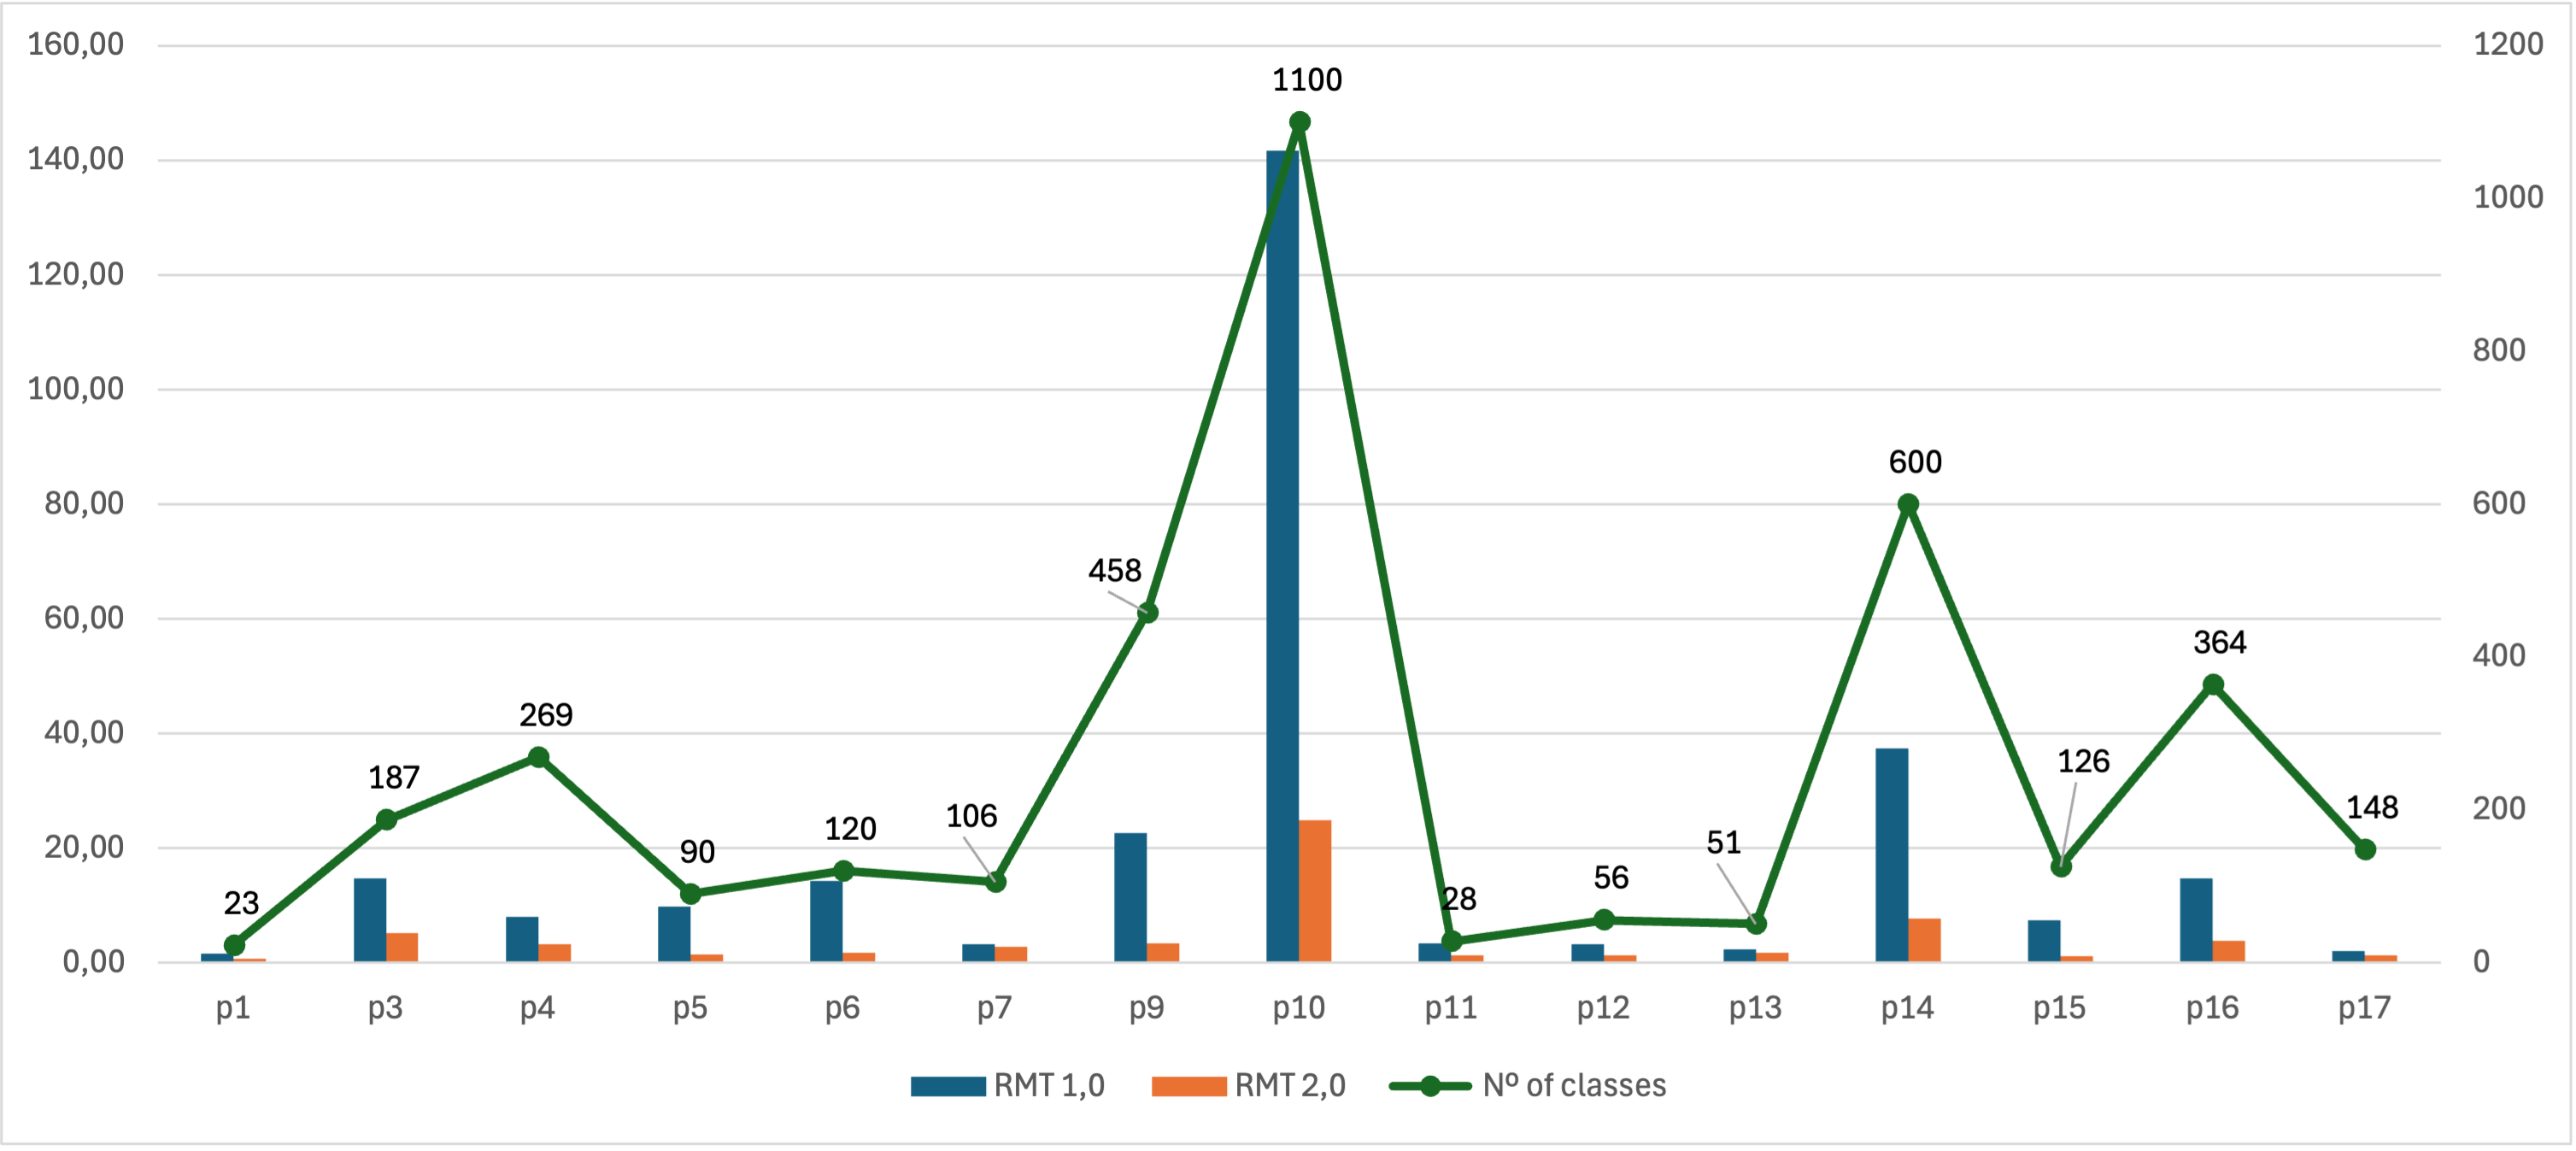
\includegraphics[width =\textwidth]{Chapter-5/Figures/time-per-project-size.png}
\SourceOrNote{Own authorship (2024)}
\end{figure}
\FloatBarrier

The projects p1, p4, p7, p13, p14, and p17 were exclusively refactored using the strategy pattern. These projects exhibit the shortest overall execution time and the slightest variance in execution duration, indicating that the strategy refactoring approach is more optimized for both tool versions. 

RMT 2.0 \footnote{Link for download \href{https://github.com/magnuspedro/spring-rmt}{RMT 2.0}} conferred numerous advantages, including improved performance, as evidenced in comprehensive analyses. The application is simple to deploy locally and, when hosted on cloud infrastructure, is universally accessible via a web browser, eliminating the need for a Java-based desktop application; this functionality extends to smartphone usage.

Even before the enhancements, the tool exhibited limitations, and few still exist. For example, when two methods within the same class require refactoring, the tool fails to distinguish between the refactoring candidates for each method. The detection and refactoring process could benefit from more parallel processing, allowing a separate process to be assigned to each method, potentially improving performance. Furthermore, the tool could be expanded with additional methods and metrics.

\textcolor{red}{achei que faltou uma conclusão geral sobre os benefícios e limitações da ferramenta 2.0. Em algum lugar deve ter o link para a ferramenta}

\section{Closing Remarks}
\label{sec-closing-results}

Upon comprehensive analysis of the datasets from both projects, it has been concluded that the proposal to enhance the tool has been successful, resulting in a 63-year improvement in the temporal efficiency of 64\%. The tool's implementation has been streamlined, necessitating containerization solutions such as Docker or Podman for execution. An automated script has been developed to compile and execute the project, concurrently deploying all required infrastructure within Docker.

%% Marcadores de PDF para capítulos subsequentes no nível principal
% \PhantomPart%

%% Formatação de elementos pós-textuais (backmatter)
%% Comando \PostTextual*: remove as seções de nível inferior às primárias do
%% sumário e dos marcadores de PDF.
\PostTextual%% Não comentar ou remover

%% Referências
\PrintReferences%

%% Glossário (elemento opcional)
%%%% Opção 1: makeindex; conforme o [Arquivo de Entradas] em \MakeGlossary.
%%%% Comando \PrintGlossary*: remove o indicativo (páginas) dos itens.
% \PrintGlossary%[\bfseries]%% Estilo de fonte do termo (opcional)
%%%% Opção 2: manual; editar o {Arquivo} para alterar.
% %%%% GLOSSÁRIO (ELEMENTO OPCIONAL)
%%
%% Relação de palavras ou expressões técnicas de uso restrito, ou de sentido
%% obscuro, utilizadas no texto, acompanhadas das respectivas definições.

%% Glossário (inserir itens em ordem alfabética)
\begin{Glossary}%[\bfseries]%% Estilo de fonte do termo
\item[biber] substituto do Bib\TeX\ para usuários do Bib\LaTeX.
  \hyperpage{40}.
\item[Bib\LaTeX] reimplementação completa das facilidades bibliográficas fornecidas pelo \LaTeX.
  \hyperpage{27}, \hyperpage{40}, \hyperpage{51}.
\item[Bib\LaTeX-abnt] pacote que oferece um estilo Bib\LaTeX\ que atende às regras da ABNT\@.
  \hyperpage{27}, \hyperpage{40}.
\item[Bib\TeX] aplicativo de gerenciamento de referências para a formatação de listas de referências no \LaTeX.
  \hyperpage{40}, \hyperpage{51}.
\glossaryspace%
\item[componente] outro exemplo de uma entrada secundária (componente), subentrada da primária chamada pai; trata-se de uma entrada irmã de outra também secundária chamada filho.
  \hyperpage{41}, \hyperpage{51}.
\glossaryspace%
\item[dissertação] trabalho acadêmico desenvolvido no mestrado.
  \hyperpage{20}, \hyperpage{28}.
\glossaryspace%
\item[equilíbrio da configuração] consistência entre os componentes.
  \hyperpage{41}.
\glossaryspace%
\item[filho] exemplo de uma entrada secundária (filho), subentrada da primária chamada pai.
  \hyperpage{41}, \hyperpage{51}.
\glossaryspace%
\item[\LaTeX] conjunto de macros para o processador de textos \TeX, utilizado amplamente para a produção de textos matemáticos e científicos devido à sua alta qualidade tipográfica.
  \hyperpage{20, 21}, \hyperpage{23}, \hyperpage{29--31}, \hyperpage{37}, \hyperpage{40, 41}, \hyperpage{44--46}, \hyperpage{51}, \hyperpage{54}.
\glossaryspace%
\item[memoir] classe \LaTeX\ que permite a composição de poesia, ficção, obras de não ficção e matemáticas, como livros, relatórios, artigos ou manuscritos.
  \hyperpage{20}, \hyperpage{25}, \hyperpage{32}, \hyperpage{45}.
\glossaryspace%
\item[pai] exemplo de entrada primária (pai) que possui subentradas ou entradas secundárias (filhos).
  \hyperpage{41}, \hyperpage{51}.
\glossaryspace%
\item[tese] trabalho acadêmico desenvolvido no doutorado.
  \hyperpage{20}, \hyperpage{28}.
\item[\TeX] sistema de tipografia criado por Donald E. Knuth.
  \hyperpage{21}, \hyperpage{41}, \hyperpage{45}, \hyperpage{51}, \hyperpage{54}.
\glossaryspace%
\item[\UTFPR-Thesis] modelo \LaTeX\ que permite atender os requisitos das normas definidas pela UTFPR para elaboração de trabalhos acadêmicos.
  \hyperpage{20}, \hyperpage{25}, \hyperpage{27}, \hyperpage{41}.
\end{Glossary}


% Parte Apêndices (elemento opcional; grupo de capítulos)
% \AppendicesPart%

%% Apêndices (elemento opcional)
\begin{Appendices}
\include{./Post-Textual/appendix-a}
\include{./Post-Textual/appendix-b}
\end{Appendices}

% Parte Anexos (elemento opcional; grupo de capítulos)
% \AnnexesPart%

%% Anexos (elemento opcional)
\begin{Annexes}
\include{./Post-Textual/annex-a}
\include{./Post-Textual/annex-b}
\end{Annexes}

%% Índice remissivo (elemento opcional)
%%%% Opção 1: makeindex (\index{...}, \Index{...}, etc.)
% \PrintIndex%
%%%% Opção 2: manual; editar o {Arquivo} para alterar.
% %%%% ÍNDICE REMISSIVO (ELEMENTO OPCIONAL)
%%
%% Lista de palavras ou frases, ordenadas segundo determinado critério, que
%% localiza e remete para as informações contidas no texto.

%% Índice remissivo (inserir itens em ordem alfabética)
\begin{RemissiveIndex}
\item \ensuremath{\vec{\nabla}} \see{operador gradiente}{999}
\item \ensuremath{\DottedCircle^0} \see{valor inicial}{999}
\item \ensuremath{\DottedCircle_\mathrm{S}} \see{fase sólida}{999}
\item \ensuremath{\theta} \see{inclinação}{999}
\item 1D \see{unidimensional}{999}
\indexspace%
\item alínea, \hyperpage{26}
\subitem subalínea, \hyperpage{26}
\item art.\ \see{artigo}{999}
\item artigo, \hyperpage{28}, \hyperpage{38}, \hyperpage{51}
\indexspace%
\item camundongo \see{rato}{999}
\item casa, \hyperpage{43}
\subitem janela, \hyperpage{43}
\subsubitem metal, \hyperpage{43}
\subitem porta, \hyperpage{43}
\subsubitem madeira, \hyperpage{43}
\item citação, \hyperpage{23, 24}, \hyperpage{27--29}, \hyperpage{41}
\subitem direta, \hyperpage{23, 24}, \hyperpage{28, 29}, \hyperpage{41}
\subitem indireta, \hyperpage{27}
\subsubitem explícita, \hyperpage{27}
\subsubitem implícita, \hyperpage{27}
\indexspace%
\item dissertação, \hyperpage{20}, \hyperpage{28}
\indexspace%
\item equilíbrio da configuração, \hyperpage{41}
\item espaçamento, \hyperpage{24}
\subitem de 1,5, \hyperpage{24}
\subitem entre linhas, \hyperpage{24}
\subitem entre parágrafos, \hyperpage{24}
\subitem simples, \hyperpage{24}
\indexspace%
\item fase sólida, \hyperpage{39}
\indexspace%
\item inclinação, \hyperpage{39}
\indexspace%
\item NBR \see{Norma Brasileira}{999}
\item Norma Brasileira, \hyperpage{22}
\item número de Reynolds, \hyperpage{39}
\indexspace%
\item operador gradiente, \hyperpage{39}
\indexspace%
\item pai, \hyperpage{41}, \hyperpage{51}
\subitem componente, \hyperpage{41}, \hyperpage{51}
\subitem filho, \hyperpage{41}, \hyperpage{51}
\indexspace%
\item ratazana \seealso{rato}{999}
\item rato, \hyperpage{43}
\subitem doméstico, \hyperpage{43}
\item \ensuremath{\mathrm{Re}} \see{número de Reynolds}{999}
\indexspace%
\item sistema operacional, \hyperpage{44}
\subitem Linux, \hyperpage{44}
\subitem macOS, \hyperpage{44}
\subitem Windows, \hyperpage{44}
\indexspace%
\item TCC \see{Trabalho de Conclusão de Curso}{999}
\item tese, \hyperpage{20}, \hyperpage{28}
\item \TeX, \hyperpage{21}, \hyperpage{41}, \hyperpage{45}, \hyperpage{51}, \hyperpage{54}
\subitem \LaTeX, \hyperpage{20, 21}, \hyperpage{23}, \hyperpage{29--31}, \hyperpage{37}, \hyperpage{40, 41}, \hyperpage{44--46}, \hyperpage{51}, \hyperpage{54}
\subsubitem biber, \hyperpage{40}
\subsubitem Bib\LaTeX, \hyperpage{27}, \hyperpage{40}, \hyperpage{51}
\subsubitem Bib\LaTeX-abnt, \hyperpage{27}, \hyperpage{40}
\subsubitem Bib\TeX, \hyperpage{40}, \hyperpage{51}
\subsubitem memoir, \hyperpage{20}, \hyperpage{25}, \hyperpage{32}, \hyperpage{45}
\subsubitem Overleaf, \hyperpage{44}
\subsubitem Papeeria, \hyperpage{44}
\subsubitem TeXlipse, \hyperpage{44}
\subsubitem Texmaker, \hyperpage{20}, \hyperpage{44}
\subsubitem {\TeX}Page, \hyperpage{44}
\subsubitem \UTFPR-Thesis, \hyperpage{20}, \hyperpage{25}, \hyperpage{27}, \hyperpage{41}
\item Trabalho de Conclusão de Curso, \hyperpage{20}
\indexspace%
\item unidimensional, \hyperpage{38}
\indexspace%
\item \ensuremath{V} \see{velocidade}{999}
\item valor inicial, \hyperpage{39}
\item velocidade, \hyperpage{39}
\end{RemissiveIndex}


%% Fim do documento
\end{document}%% Não comentar ou remover

%% Observação: o arquivo final (PDF) pode ser convertido para PDF/A usando
%% diversas ferramentas, por exemplo:
%%   https://www.pdfforge.org/online/en/pdf-to-pdfa
